%% main_paper_NN34.tex
%% MDPI MAKE 投稿用日本語草稿
%% AE/VAEにおける有効潜在次元の診断的解釈（版34）
%% 版34の変更点：Review_codex33.txt（Major 1--8, Minor 1--10）への対応と分量削減
%%   - 貢献の一文化＋既存研究との対比表（Major 1）
%%   - mknee の要約記述を「TwoNN 由来探索窓に条件付けられた局所精密化」に統一（Major 2）
%%   - Fashion-MNIST を付録の探索的補助証拠に降格（Major 3）
%%   - TwoNN の安定性/バイアス区別を前倒し・要約部の表現統制（Major 4）
%%   - tau_eff 議論をヒューリスティックな外挿と明示・操作的定義を追加（Major 5）
%%   - Abstract 短縮，反復削減，単一シード実験の付録移動（Major 6, Minor 1, 5）
%%   - stable identification を「報告基準（reporting criteria）」と明示（Major 7）
%%   - 再現性情報の具体化（前処理・最適化・データ分割・コード公開）（Major 8）
%%   - 対象量と推定量の対応表を §3 冒頭に追加（Minor 2）ほか
%% コンパイル: platex main_paper_NN34.tex && dvipdfmx main_paper_NN34.dvi

\documentclass[11pt,a4paper]{jsarticle}

\usepackage{amsmath,amsthm,amssymb}
\usepackage{mathtools}
\usepackage[dvipdfmx]{graphicx}
\usepackage{booktabs}
\usepackage{url}
\usepackage{here}
\usepackage{array}
\usepackage{multirow}
\usepackage{enumerate}
\usepackage[margin=25mm]{geometry}
\usepackage[dvipdfmx,hidelinks]{hyperref}
\usepackage{caption}

%% 定理環境
\newtheorem{theorem}{定理}
\newtheorem{proposition}{命題}
\newtheorem{definition}{定義}
\newtheorem{remark}{注意}
\newtheorem{corollary}{系}

%% 記号略記
\newcommand{\dID}{d_{\mathrm{ID}}}
\newcommand{\dz}{m}
\newcommand{\dzopt}{m^{\mathrm{cand}}}
\newcommand{\dtrue}{d_{\mathrm{true}}}
\newcommand{\Jg}{J_g}
\newcommand{\R}{\mathbb{R}}
\newcommand{\kap}{\kappa}
\newcommand{\AUsat}{\mathrm{AU}_{\mathrm{sat}}}
\newcommand{\dzsat}{m^{\mathrm{sat}}}
\newcommand{\mknee}{m^{\mathrm{knee}}}
\newcommand{\demb}{d_{\mathrm{emb}}}

%% ===================================================================
\title{AE/VAE における有効潜在次元の診断的解釈}
%% 英語タイトル候補：
%%   Diagnostic Interpretation of Effective Latent Dimensionality in
%%   Autoencoders and Variational Autoencoders
%%   （または）
%%   Interpreting Effective Latent Dimensionality in AE/VAE Models via
%%   Active-Unit Dynamics and Intrinsic Dimension Estimation
\author{（著者名）\\
{\small （所属機関）}\\
{\small \texttt{（メールアドレス）}}}
\date{}

\begin{document}
\maketitle

%% ===================================================================
\begin{abstract}
本論文では，AE/VAE の潜在表現が実際に利用する有効潜在次元を診断的に解釈するための
多指標診断フレームワークを提案する．
本フレームワークは，性質の異なる複数の対象量——KL 活性座標数（AU 値）と
潜在表現の内在次元（TwoNN/MLE ID）——を混同せずに区別し，
AU 値を頑健な直接観測指標（頑健＝本実験条件でのシード間分散が小さいこと），
TwoNN/MLE ID を数値的に安定な補助的参照推定量，
AU 鈍化点$\mknee$を探索的変化点として運用する指標分類論を与える．
理論面では，線形ガウス rate-distortion 近似のもとで
第$j$固有方向の活性化条件$\lambda_j > \beta\tau^2$を導出する（解釈的サロゲート）．
実験面では，MNIST FC-VAE で AU 値と TwoNN ID の高い多シード再現性を確認する一方，
$\mknee$は疎グリッドで大きく変動し，
\textbf{TwoNN 由来の探索窓に条件付けられた局所精密化}としてのみ
$\mknee = 10.3 \pm 0.9$に安定化することを示す（TwoNN と独立な検証ではない）．
さらに Conv-VAE・自然画像実験により，AU/$\mknee$ 診断が困難となる境界条件を定量化する．
検証範囲等の詳細な限定条件は §\ref{sec:intro_structure} に明示する．
\end{abstract}

%% ===================================================================
\section{まえがき}\label{sec:intro}

\subsection{研究背景：有効潜在次元の解釈という問題}\label{sec:intro_bg}

表現学習において，オートエンコーダ（Autoencoder; AE）および
変分オートエンコーダ（Variational Autoencoder; VAE）\cite{kingma2014vae}は，
高次元データから低次元の潜在表現（latent representation）を学習する
中核的な非教師あり学習モデルである\cite{bengio2013representation}．
この潜在表現の「質」を規定する最も基本的な設計パラメータが
ボトルネック次元（bottleneck dimension）$m$である：
$m$が小さすぎると情報が欠落し，大きすぎると
冗長な次元が生じる（VAE では posterior collapse\cite{lucas2019elbo}が悪化する）．

しかし，学習された潜在表現が「実際に何次元を有効に使っているか」——
すなわち\textbf{有効潜在次元（effective latent dimensionality）}——を
定量的に読む方法論は，深層表現学習の研究において十分に確立されていない．
既存研究\cite{ansuini2019intrinsic,valeriani2023geometry}は
深層ネットワークの各層の内在次元を測定してきたが，
AE/VAE のボトルネックにおける有効次元を，その学習ダイナミクスとともに
系統的に分析した研究は限られている．

本論文が取り組む中核的な問いは：
\begin{quote}
\textit{AE/VAE は，入力データの内在次元（local intrinsic dimensionality）や
位相的埋め込み次元（topological embedding dimensionality）をどのように
潜在空間の有効次元として「学習」するか？
そして，その有効次元を外から定量的に読む方法はあるか？}
\end{quote}

\subsection{本研究の位置づけと貢献}\label{sec:intro_aim}

本論文の中心的貢献を一文で述べると次のとおりである：
\begin{quote}
\textbf{本研究の新規性は，新しい次元推定量の提案ではなく，
既知の構成要素（AU 値，TwoNN/MLE ID，MSE エルボー，PCA）を
「頑健指標／補助的参照／探索的指標」という運用上の分類論（operational taxonomy）として整理し，
各指標がいつ安定でいつ破綻するかを実験的に境界づけた点にある．}
\end{quote}
「$\mknee$ により適切なボトルネック次元を一意に同定できる」という主張は行わない——
主要な有効次元の読み取りは頑健指標（AU 値）と
数値安定な補助的参照推定量（TwoNN ID）が担う（表\ref{tab:indicator_class}）．
既存研究との対比を表\ref{tab:novelty}に示す．

\begin{table}[H]
\centering
\caption{Positioning relative to prior work: known ingredients vs.\ contributions of this paper.}
\label{tab:novelty}
\small
\begin{tabular}{p{3.6cm}p{4.9cm}p{5.6cm}}
\toprule
Ingredient & Prior work & This paper \\
\midrule
AU / posterior collapse & Qualitative analysis in linear VAEs \cite{lucas2019elbo} & Multi-seed reproducibility of AU$(m)$ dynamics across $m$-grids; slowdown point $\mknee$ and its instability characterization \\
TwoNN / MLE ID & Estimators \cite{facco2017twonn,levina2005mle}; measuring trained networks \cite{ansuini2019intrinsic,pope2021intrinsic} & Stability-vs-bias separation as a latent-space auxiliary reference; dominant stability condition $m \gg \hat{d}_\mathrm{ID}$ (Exp-Real-Geom) \\
$\beta$-VAE activation & PPCA at $\beta=1$ \cite{tippingbishop1999ppca}; qualitative $\beta$ effects \cite{higgins2017betavae,lucas2019elbo} & Closed-form threshold $\lambda_j > \beta\tau^2$ under a linear-Gaussian rate-distortion surrogate (Theorem \ref{thm:linear_vae}) \\
Indicator combination & Individual indicators used in isolation & Operational taxonomy (robust / auxiliary / exploratory) with quantified validity ranges and boundary conditions \\
\bottomrule
\end{tabular}
\end{table}

具体的な\textbf{貢献は以下の3点}である：
\begin{enumerate}
  \item \textbf{多指標診断フレームワーク（運用上の分類論）}：
        AU 値を頑健指標，TwoNN ID を数値安定な補助的参照推定量，
        $\mknee$を探索的変化点として区別する枠組みを与える（§\ref{sec:framework}）．
        MNIST 3シード検証で AU 値（$\sigma \leq 0.5$）と TwoNN ID（$10.03 \pm 0.12$）の
        再現性を確認し，\textbf{TwoNN 由来の探索窓に条件付けられた局所精密化}として
        $\mknee = 10.3 \pm 0.9$（Exp-Mnist-Dense-300，§\ref{sec:exp_el}）を得る
        （TwoNN と独立な検証ではない；検証範囲は MNIST FC-VAE・$\beta = 4$・3シード）．
  \item \textbf{線形ガウス rate-distortion 近似に基づく AU 活性化条件}：
        活性化条件$\lambda_j > \beta\tau^2$を水充填定理と KKT 条件から導出する
        （定理\ref{thm:linear_vae}，§\ref{sec:theory}）．
        非線形 VAE の厳密定理ではなく，非線形実験との定性的対応を与える解釈的サロゲートである．
  \item \textbf{適用可能範囲と境界条件の定量化}：
        「等長性改善より$m \gg \hat{d}_\mathrm{ID}$が TwoNN 安定性の支配的条件」
        （Exp-Real-Geom，命題\ref{thm:twonn_stability}）を実証し，
        Conv-VAE・自然画像で AU/$\mknee$ 診断が困難となる境界条件を
        報告基準（reporting criteria）5条件として定量化する
        （§\ref{sec:disc_convvae}，§\ref{sec:disc_limitation}）．
\end{enumerate}

\subsection{「次元」の2種類：局所的固有次元と位相的埋め込み次元}\label{sec:intro_dim}

本論文では多様体の「次元」として$\dID$（局所的固有次元：TwoNN/MLE の推定対象）と
$\demb$（位相的最小埋め込み次元：自己交差なく埋め込むための最小次元）を区別する
（Swiss Roll では$\demb = \dID = 2$，Torus では$\demb = 3 > \dID = 2$）．

ただし，\textbf{本論文の主貢献は$\dID$や$\demb$との対応を証明することではなく，
AU 値・TwoNN ID・$\mknee$という診断指標の頑健性・限界・適用条件の整理にある}．
$\demb$と$\AUsat$との条件付き対応（Torus・Möbius 等）は付随的観察として補助に位置づける
（§\ref{sec:disc_incidental}）．

\subsection{リサーチクエスチョン}\label{sec:intro_rq}

\begin{description}
  \item[RQ1] VAE の AU Dynamics から得られる変化点$\mknee$は，どのようなグリッド密度・シード数・
             アーキテクチャ条件のもとで，TwoNN/MLE による ID 推定値と整合する診断補助量として
             利用可能か．
  \item[RQ2] AE/VAE の有効潜在次元を多指標（AU 値，TwoNN/MLE，MSE エルボー，PCA）で
             解釈するフレームワークは，単一指標に対して相補的な情報を提供するか．
  \item[RQ3] ボトルネック余裕（$m / \hat{d}_\mathrm{ID}$ の大小）および幾何的正則化（IsometricAE）は，
             TwoNN ID 推定の安定性にどのような影響を与えるか．
\end{description}

\subsection{本論文の構成}\label{sec:intro_structure}

\textbf{検証範囲の明示}：
本論文の検証は合成多様体（$d_{\mathrm{true}} \leq 3$）・MNIST・Fashion-MNIST（全結合型 AE/VAE），
Conv-AE/VAE，および自然画像（CIFAR-10・SVHN）を対象とする．
自然画像実験では TwoNN 補助推定が Pope ら\cite{pope2021intrinsic}の報告値と整合することを確認し，
Conv-VAE における AU/$\mknee$ 診断の適用可能範囲と限界条件を定量化する
（フレームワーク全体の自然画像への「汎化」を主張するものではない）．

§\ref{sec:related}（関連研究），§\ref{sec:framework}（フレームワーク），
§\ref{sec:theory}（理論的背景；定理\ref{thm:linear_vae}含む），
§\ref{sec:exp}（実験），§\ref{sec:discussion}（考察），§\ref{sec:conclusion}（むすび）の順で構成する．
詳細な証明と感度分析は付録にまとめる．

%% ===================================================================
\section{関連研究}\label{sec:related}

\subsection{表現学習とオートエンコーダ}\label{sec:related_ae}

Bengio ら\cite{bengio2013representation}は表現学習の理論的枠組みを整理し，
AE が多様体仮説\cite{fefferman2016manifold}に基づいて
高次元データの低次元構造を学習する機構を論じた．
$\beta$-VAE\cite{higgins2017betavae}は KL 正則化の重み$\beta$を大きくすることで
Disentangled 表現を促進し，AU に直接影響する
（posterior collapse の線形 VAE 解析は§\ref{sec:related_au}で述べる）．
DAE\cite{alain2014dae}はスコアマッチングの観点から，
Denoising Autoencoder の再構成方向が多様体の法線方向を選択的に抑制することを示した．
CAE\cite{rifai2011cae}はエンコーダ側ヤコビアンの正則化により収縮的表現を学習する．

\subsection{深層表現の内在次元解析}\label{sec:related_id}

Pope ら\cite{pope2021intrinsic}は自然画像の内在次元が
TwoNN 推定で画素次元よりはるかに低いことを示した
（CIFAR-10: $d_\mathrm{ID} \approx 26$ at $32 \times 32$）．
Ansuini ら\cite{ansuini2019intrinsic}は深層ネットワークの各層を通じて
ID が変化するパターンを定量化し，表現の収縮・拡張現象を記録した．
Valeriani ら\cite{valeriani2023geometry}は大規模変換器モデルの隠れ表現の
幾何構造を系統的に解析した．
Birdal ら\cite{birdal2021intrinsic}は持続的ホモロジーと ID の統合による
汎化誤差との関係を分析した．
本研究はこれらの「既存のネットワークの ID を測る」研究と相補的であり，
AE/VAE の\textbf{設計段階}および\textbf{学習ダイナミクス}における有効次元の形成を追跡する点で異なる．

内在次元推定手法としては，TwoNN\cite{facco2017twonn}（2近傍距離比）と
MLE\cite{levina2005mle}（最尤推定）を採用する．
DANCo\cite{ceruti2014danco}はより精密だが計算コストが高い．
なお，非線形次元削減の可視化手法として UMAP\cite{mcinnes2018umap}が広く用いられるが，
本研究は可視化ではなくボトルネック次元の\textbf{定量的な解釈}に焦点を当てる．

\subsection{Active Units と Posterior Collapse}\label{sec:related_au}

Active Unit（AU）\cite{lucas2019elbo,higgins2017betavae}は，
VAE の事後平均の分散が閾値$\delta$を超える潜在次元の数であり，
KL 正則化が有効に機能している次元数を定量化する指標である．
Lucas ら\cite{lucas2019elbo}は，ELBO の最小化が posterior collapse を引き起こす条件を
線形 VAE の枠組みで分析し，AU とデータの固有値構造との関連を定性的に論じた．
一方，本研究の定理\ref{thm:linear_vae}は Lucas らの定性的議論を，
データ固有値$\lambda_j$・ノイズ$\tau^2$・正則化$\beta$による
\textbf{閉形式しきい値$\lambda_j > \beta\tau^2$として定量化}し，
さらに Shannon の水充填定理との明示的な結びつきと KKT 条件を用いて，
線形ガウス rate-distortion 近似のもとで定量的導出を行う点が新規性である
（Tipping \& Bishop~\cite{tippingbishop1999ppca}の PPCA における$\beta=1$の特殊ケースも統合する）．
また，実データにおける AU 増加ダイナミクスの系統的な分析，特に$\mknee$という概念とその
有効表現次元との対応・限界条件・安定化戦略については，本研究が体系的に検証する
（定理\ref{thm:linear_vae}，命題\ref{thm:mknee_instab}，§\ref{sec:disc_mknee_improve}）．

\subsection{幾何的オートエンコーダ}\label{sec:related_geo}

Nazari ら\cite{nazari2023geometric}は幾何的オートエンコーダを提案し，
エンコーダが多様体の幾何構造を保存するための正則化を導入した．
Kato ら\cite{kato2020rdae}はデコーダのヤコビ行列に対するプルバック計量の
単位行列への近似化により等長埋め込みを実現する IsometricAE を提案した．
本研究では IsometricAE を「有効次元の読み取り精度の前提条件（等長性）を
改善する補助ツール」として位置づける（RQ3，実験 Exp-Syn-Iso）．

%% ===================================================================
\section{フレームワーク：有効潜在次元の読み取り}\label{sec:framework}

\subsection{問題設定と主要記号}\label{sec:framework_setup}

AE/VAE を入力次元$N$，ボトルネック次元$m$で定義する：
エンコーダ$f: \R^N \to \R^m$，デコーダ$g: \R^m \to \R^N$．
VAE ではエンコーダが事後分布$q_\phi(z|x) = \mathcal{N}(\mu(x), \sigma^2(x))$を出力し，
KL 正則化（強度$\beta$）が情報ボトルネックとして作用する．

\textbf{Active Unit（AU）}の定義：
\begin{equation}
  \mathrm{AU}(m) = \sum_{k=1}^{m} \mathbf{1}\bigl[\mathrm{Var}_x[\mu_k(x)] > \delta\bigr],
  \quad \delta = 10^{-2}
  \label{eq:au_def}
\end{equation}
ただし$\mu_k(x)$は事後平均の第$k$成分，$\delta$は閾値（Lucas ら\cite{lucas2019elbo}に準拠）．
この閾値選択に対して AU は極めて頑健であり，$\delta \in [10^{-3}, 10^{-1}]$の範囲で AU 値はほぼ変化しないことを感度分析で確認している（\ref{app:delta}参照）．

\textbf{AU 増加率の定義（2段階）}：
まずグリッド上の生の増加率$s(m_i)$を，
\begin{equation}
  s(m_i) = \frac{\mathrm{AU}(m_i) - \mathrm{AU}(m_{i-1})}{m_i - m_{i-1}}
  \label{eq:au_raw_rate}
\end{equation}
と定義する（$m_{i-1}$はグリッド上の直前の値）．
次に，正規化増加率$\rho(m_i)$を，
\begin{equation}
  \rho(m_i) = \frac{s(m_i)}{\max_j s(m_j)}
  \label{eq:au_rate}
\end{equation}
と定義する（$\rho(m_i) \in [0, 1]$）．

\textbf{主要記号一覧}を表\ref{tab:notation}に示す．

\begin{table}[H]
\centering
\caption{Notation used throughout this paper}
\label{tab:notation}
\small
\begin{tabular}{lll}
\toprule
Symbol & Meaning & Section \\
\midrule
$m$ & Bottleneck dimension (design parameter) & §\ref{sec:framework} \\
$\dzopt$ & Diagnostic candidate dimension (not a unique optimum) & §\ref{sec:framework} \\
$\dzsat$ & AU sharp saturation point (diagnostic candidate for synthetic manifolds) & §\ref{sec:framework} \\
$\mknee$ & AU slowdown point (rough heuristic for real data) & 式\eqref{eq:mknee} \\
$\AUsat$ & Maximum AU value over the grid & 式\eqref{eq:au_def} \\
$\hat{\dID}$ & ID estimate via TwoNN/MLE & §\ref{sec:framework} \\
$\dtrue$ & True intrinsic dimension of synthetic manifold (known) & §\ref{sec:exp_synthetic} \\
$\demb$ & Topological minimum embedding dimension ($\demb \geq \dID$) & §\ref{sec:intro_dim} \\
$\kap$ & Decoder Jacobian condition number (isometry indicator) & §\ref{sec:related_geo} \\
$s(m_i)$ & Raw AU increase rate per unit dimension & 式\eqref{eq:au_raw_rate} \\
$\rho(m_i)$ & Normalized AU increase rate ($\in[0,1]$) & 式\eqref{eq:au_rate} \\
$\tau_{\mathrm{knee}}$ & Slowdown detection threshold (default: 0.25) & 式\eqref{eq:mknee} \\
\bottomrule
\end{tabular}
\end{table}

本フレームワークの核心は，各指標を\textbf{頑健指標}と\textbf{探索的指標}に明示的に分類した上で
相補的に活用する点にある（表\ref{tab:indicator_class}）．
この分類は，後述の実験的知見（§\ref{sec:exp_multiseed2}）に基づく実証的分類であり，
単一指標への過信が招く誤診断を体系的に回避する設計思想の中核をなす．

\textbf{「頑健指標」と「探索的指標」の意味について}：
ここでいう「頑健」とは，真の内在次元に対して不偏であることを意味しない．
少なくとも本実験条件下で乱数シードに対する分散が小さいという意味で用いる．
一方，「探索的」とは，グリッド設計や仮説生成には有用であるが，
有効潜在次元の一意な推定値としては扱わないことを意味する．

\begin{table}[H]
\centering
\caption{Classification and empirical reliability of diagnostic indicators. Throughout this paper, ``robust'' means \textit{low inter-seed variance under our experimental conditions}, not unbiasedness with respect to the true intrinsic dimension.}
\label{tab:indicator_class}
\small
\begin{tabular}{p{3.3cm}p{3.1cm}p{3.9cm}p{4.0cm}}
\toprule
Indicator & Category & Empirical reliability (inter-seed $\sigma$) & Primary use \\
\midrule
AU values ($\mathrm{AU}(m)$) & \textbf{Robust indicator} & $\sigma \leq 0.5$ (MNIST 300ep) & Direct observation of effective dimensionality; independent of reference AE geometry (depends on $\beta$, $\delta$, model capacity) \\
TwoNN ID ($\hat{d}_\mathrm{ID}$) & \textbf{Numerically stable auxiliary reference}$^\dagger$ & $\sigma \leq 0.12$ ($m=64$) & Reference estimate of intrinsic dimension \\
MSE elbow & Auxiliary indicator & Qualitative only & Reconstruction-side verification \\
PCA cumulative variance & Auxiliary indicator & Linear assumption only & Linear baseline \\
$\mknee$ (AU slowdown point) & \textbf{Exploratory indicator} & $\sigma=15$ (sparse grid); $\sigma=0.9$ (dense grid) & Rough heuristic of effective dimensionality \\
\bottomrule
\end{tabular}
\medskip
\footnotesize
$^\dagger$ TwoNN ID is a \textbf{supplementary reference estimator} subject to isometry bias ($\kap \approx 10^9$); see §\ref{sec:framework_pipeline} for details.
$\sigma$ of $\mknee$ is for sparse grid; improved to $\sigma=0.9$ with dense grid (Exp-Mnist-Dense), where grid design is a major factor (§\ref{sec:exp_el}).
\normalsize
\end{table}

\subsubsection*{各指標が推定する対象量の区別}\label{sec:framework_targets}

「有効潜在次元」という語のもとで実際には性質の異なる複数の量が測られる．
誤診断を避けるため，本稿では5つの対象量とそれぞれの推定量・観測量を
表\ref{tab:target_estimator}のとおり明示的に区別する．

\begin{table}[H]
\centering
\caption{Target quantities vs.\ estimators/observables. The paper's claims are stated on top of these distinctions.}
\label{tab:target_estimator}
\small
\begin{tabular}{p{4.6cm}p{4.3cm}p{4.8cm}}
\toprule
Target quantity & Estimator / observable & Status \\
\midrule
(i) Intrinsic dim.\ of the data manifold $d_\mathrm{ID}^\mathrm{data}$ & Known $\dtrue$ (synthetic); input-space TwoNN/MLE (real data) & Approximation only; no claim beyond synthetic cases \\
(ii) Intrinsic dim.\ of the latent representation $d_\mathrm{ID}^\mathrm{latent}$ & TwoNN/MLE on reference-AE latents (our $\hat{d}_\mathrm{ID}$) & Numerically stable \textbf{latent-side reference}; may differ from (i) via embedding distortion (§\ref{sec:disc_twonn_bias}) \\
(iii) Number of KL-active coordinates & AU value; change point $\mknee$; max $\AUsat$ & Observable of coordinate usage; depends on $\beta$, $\delta$, architecture; \textbf{not} an ID estimator \\
(iv) Bottleneck dim.\ required for reconstruction & MSE elbow (qualitative) & Reconstruction-side reference \\
(v) Diagnostic candidate dimension $\dzopt$ & Designer's choice cross-checking (i)--(iv) & Not a unique optimum \\
\bottomrule
\end{tabular}
\end{table}

本稿の主張はこの区別の上に述べられる：
定理\ref{thm:linear_vae}は線形サロゲートにおける（iii）の閾値を与え，
命題\ref{thm:twonn_stability}と実験 Exp-Real-Geom は（ii）の安定条件を扱い，
$\mknee$の安定化結果（§\ref{sec:exp_el}）は（iii）の変化点が（ii）の近傍に安定化する条件を特定する．
（i）そのものへの言明は合成多様体（$\dtrue$既知）の場合を除き行わない．

\subsection{有効潜在次元の読み取りパイプライン}\label{sec:framework_pipeline}

本研究が提案するフレームワークは，
「AE/VAE が学習する有効潜在次元を2段階で読み取る」解釈パイプラインである（図\ref{fig:framework}）．

\textbf{Stage 1：内在次元の近似推定（補助的役割）}

本論文では，内在次元$\hat{d}_\mathrm{ID}$の推定を2通りの方法で行う：
（a）\textbf{合成多様体}では入力空間に直接 TwoNN/MLE を適用（$\dtrue$との対比が可能）；
（b）\textbf{実データ（MNIST 等）}では，高次元の呪いを回避するため，
大きめの参照 AE（$m_{\mathrm{ref}} = 256$）の潜在表現を経由して推定する．

\textbf{限界の明示}：方法（b）の参照 AE（$m = 256 \gg \hat{d}_\mathrm{ID}$）の潜在空間は
等長性を保証しておらず（$\kap \approx 10^9$；§\ref{sec:disc_limitation}），
得られた$\hat{d}_\mathrm{ID}$は\textbf{数値的には安定だが等長性バイアスを含みうる}近似値である
（安定性と正確性の区別は§\ref{sec:disc_twonn_bias}）．
本論文では$\hat{d}_\mathrm{ID}$を候補範囲を示す補助的な事前情報として扱い，
主要な読み取りは Stage 2 の AU Dynamics に委ねる．
複数の$m$値（例：$\{64, 128, 256\}$）での推定値の収束確認により実用上の安定性を担保する．

\textbf{Stage 2：AU Dynamics による有効次元の読み取り}

ボトルネック次元$m$を離散グリッド
$\mathcal{M} = \{1, 2, 4, 8, 12, 16, 20, 32, 64, 128, 256\}$上でスイープし，
各$m$で VAE（$\beta = 4$）を学習して AU$(m)$を計算する
（実験によっては$\mathcal{M}$の一部の$m$点を省略・追加した拡張グリッドを用いる；各実験節に明記する）．
AU パターンに応じて診断候補次元$\dzopt$の読み取り方を使い分ける
（\textbf{$\dzopt$はボトルネック次元の唯一の「最適値」ではなく，多指標による診断上の候補次元である}）：

\begin{description}
  \item[飽和型（合成多様体などシンプルなデータ）]
        AU が特定の$m$で急激に飽和する場合，その飽和点$\dzsat$を
        診断候補次元$\dzopt = \dzsat$として用いる
        （AU 値が頑健なため，この条件ではかなり信頼性が高い）．
  \item[漸増型（実データ，MNIST 等）]
        AU が$m$とともに緩やかに増加する場合，鈍化点$\mknee$を
        粗い設計目安として参照する（探索的指標）：
        \begin{equation}
          \mknee = \min\{m_i \in \mathcal{M} : \rho(m_i) < \tau_{\mathrm{knee}}\}
          \label{eq:mknee}
        \end{equation}
        ただし$\tau_{\mathrm{knee}} = 0.25$（デフォルト；\ref{app:tau_knee}参照）．
        $\mknee$は「VAE が最初に有意な次元圧縮を行う点」を粗く捉えるが，
        数値は$m$グリッドや乱数シードに依存するため，
        AU 値・TwoNN ID と照合して最終的に判断する（§\ref{sec:disc_mknee}）．
        $\mknee$と$\hat{d}_\mathrm{ID}$が整合しなくてもフレームワーク全体が無効になるわけではない．
\end{description}

CKA\cite{kornblith2019cka}および MSE エルボーを補助基準として多指標で総合的に判断する．
なお MSE エルボーは MSE$(m)$曲線の目視による定性的参照であり，
\textbf{本稿はアルゴリズミックな肘点検出器を提案しない}（表\ref{tab:target_estimator}の（iv））．

\begin{figure}[H]
\centering
\renewcommand{\arraystretch}{1.4}
\begin{tabular}{c}
  \fbox{\textbf{入力データ} $\boldsymbol{X} \in \R^N$（多様体仮説のもと）} \\[3pt]
  $\Big\downarrow$ \\[1pt]
  \fbox{\parbox{0.70\linewidth}{\centering
    \textbf{Stage 1：有効内在次元の近似推定}\\[1pt]
    合成多様体（$\dtrue$既知）でベンチマーク → TwoNN/MLE を選択\\
    実データ：参照 AE（$m_{\mathrm{ref}} = 256$）の潜在表現で TwoNN/MLE を適用\\
    $\Rightarrow$ 推定値 $\hat{\dID}$（候補範囲の目安，近似値）
  }} \\[3pt]
  $\Big\downarrow$ \\[1pt]
  \fbox{\parbox{0.70\linewidth}{\centering
    \textbf{Stage 2：AU Dynamics による有効次元の診断}\\[1pt]
    グリッド$\mathcal{M}$上で VAE をスイープ → AU$(m)$ を追跡\\
    飽和型：診断候補 $\dzopt = \dzsat$（信頼性高），漸増型：粗い目安 $\dzopt = \mknee$（探索的）\\
    \textbf{主要指標}：AU 値（頑健指標）・TwoNN ID（数値安定な補助的参照）\\
    \textbf{$\mknee$は探索的目安であり，一意な最適値ではない}
  }} \\[3pt]
  $\Big\downarrow$ \\[1pt]
  \fbox{\parbox{0.70\linewidth}{\centering
    \textbf{補助（RQ3）：幾何的正則化・ボトルネック余裕と TwoNN 安定性の確認}\\[1pt]
    $m \gg \hat{d}_\mathrm{ID}$の条件確認 → TwoNN 補助推定の適用条件（validity range）を評価
  }}
\end{tabular}
\caption{Diagnostic pipeline for effective latent dimensionality. The diagnostic candidate dimension $\dzopt$ is not a unique optimal solution but a candidate based on multiple indicators (AU values, TwoNN ID, $\mknee$).}
\label{fig:framework}
\end{figure}

\subsection{$\mknee$ の解釈的意義}\label{sec:framework_mknee_interp}

KL 正則化は再構成に不要な余剰潜在次元を非活性化する
（posterior collapse を誘導する）\cite{lucas2019elbo,higgins2017betavae}．
$m < \hat{d}_\mathrm{ID}$では全次元が活性化され（$\mathrm{AU}(m) \approx m$），
$m$が$\hat{d}_\mathrm{ID}$を超えると余剰次元への KL 圧力により AU 増加率が鈍化する——
$\mknee$はこの鈍化を粗く捉える変化点である．
ただし数値的再現性は$m$グリッドや乱数シードに依存し保証されない
（§\ref{sec:exp_multiseed2}，§\ref{sec:disc_mknee}）．
$\mknee$の整合有無にかかわらず，AU 値と TwoNN ID の組み合わせによる読み取りが
本フレームワークの中心である．

\subsection{Stable Identification の報告基準（reporting criteria）}\label{sec:natimg_stable_id}

新しいデータセット・アーキテクチャで「AU/$\mknee$ を安定同定できた」と報告するための
基準を，実験に先立ってここで定義する．
これらは一般的に有効な「安定同定の判定基準」ではなく，
MNIST FC-VAE の挙動から校正された\textbf{本研究内の報告基準（reporting criteria）}である．
本論文では以下の5条件を全て満たす場合を \textbf{stable identification} と呼ぶ：

\begin{enumerate}
  \item \textbf{シード安定性}：3〜5 シードで$\mknee$の標準偏差$\sigma_\mathrm{seed} \leq 0.1 \cdot \mknee$
  \item \textbf{グリッド安定性}：グリッドを 2 倍密にしても$\mknee$の変動$\leq 20\%$
  \item \textbf{$\beta$安定性}：$\beta_{\max}$を$\pm 20\%$変化させても$\mknee$が同じグリッドセルに収まる
  \item \textbf{AU プラトー安定性}：AU プラトー値のシード間$\sigma \leq 0.05 \cdot \AUsat$
  \item \textbf{TwoNN・AU 整合性}：$\mknee \leq 3 \hat{d}_\mathrm{ID}$（TwoNN と AU の粗い整合）
\end{enumerate}

これらの閾値（$0.1\cdot\mknee$，$20\%$，$0.05\cdot\AUsat$，$3\hat{d}_\mathrm{ID}$）は
理論的に導出された普遍定数ではなく，\textbf{著者らが定めた報告基準}であり，
本研究の範囲を超えた一般的な安定同定基準としての意味は主張しない．
数値の選択は，MNIST FC-VAE で観測されたシード間変動のスケール
（AU：$\sigma \leq 0.5$，密グリッド$\mknee$：$\sigma = 0.9 \approx 0.09\mknee$；§\ref{sec:exp_el}）を
「安定」の目安とし，それを桁で大きく超える変動を「不安定」と判定できるよう丸めた値である．
閾値自体の系統的な感度分析は今後の課題であるが，
本稿の結論（自然画像では5条件のいずれも未達；§\ref{sec:exp_natimg_sweep}）は
閾値を2倍に緩めても変わらない程度に判定が明確である．
本基準の目的は「成功」の宣言ではなく，
安定同定が達成できない場合に\textbf{どの条件が破れているか}を分解して記述することにある．

%% ===================================================================
\section{理論的背景}\label{sec:theory}

本章では，フレームワークを支える理論的基盤を示す．
命題\ref{thm:lower_bound}は位相次元と埋め込み次元に関する標準的な位相的事実に基づく下界であり，
厳密な主張は「ゼロ再構成誤差を達成するために必要な次元」という理想化された前提に限定される．
\textbf{定理\ref{thm:linear_vae}}は線形ガウス rate-distortion 近似における解析的結果であり，
AU 活性化しきい値を閉形式で与える（証明詳細は\ref{app:proofs}）．
命題\ref{thm:mknee_instab}は理想化された単調飽和モデル下での補題であり，
実際の非線形設定では上界を超えた誤差が生じうる点に注意．
命題\ref{thm:twonn_stability}は不偏性の保証ではなく，条件付き安定性の十分条件のスケッチである．
命題\ref{thm:pullback}は等長性の定義から直接導かれる．

\begin{proposition}[ボトルネック次元の位相的下界]\label{thm:lower_bound}
滑らかな$d$次元多様体$\mathcal{M} \subset \R^N$を
連続な AE により自己交差なく再構成し，理想的にゼロ再構成誤差を達成するためには，
ボトルネック次元$m \geq d$が必要である．
（有限サンプル・有限容量・近似的再構成を含む実際の設定は対象外の理想化である．）
\end{proposition}

\begin{proof}
ゼロ再構成誤差には$g \circ f|_\mathcal{M}$が恒等写像に近い必要があり，
$f|_\mathcal{M}: \mathcal{M} \to \R^m$が連続な単射でなければならない．
$d$次元多様体から次元$m < d$のユークリッド空間への連続単射は
位相的埋め込み次元の標準的な性質（Hatcher~\cite{hatcher2002algebraic}，第 2 章）により存在しないため，
$m \geq d$が必要条件となる．
\end{proof}

本命題は$\hat{d}_\mathrm{ID}$がボトルネック次元の原理的下界の参照点として機能することを正当化する
（実用上は「有効次元の候補範囲」として用いる）．
実験 Exp-Syn-1 では，$m = 1 \to 2$の遷移で MSE が Swiss Roll において約 35 倍改善することで確認される（§\ref{sec:exp_synthetic}）．

%% ─── 定理1：線形β-VAEのAU飽和しきい値 ────────────────────────────────────
\begin{remark}[既存研究との関係]
本定理は既知の解析群——Lucas et al.~\cite{lucas2019elbo}の線形 VAE における posterior collapse の議論，
Tipping \& Bishop~\cite{tippingbishop1999ppca}の PPCA（$\beta = 1$の特殊ケースに相当），
Shannon の水充填定理\cite{cover2006elements}——と密接に関連しており，
新規性はこれらを$\beta \neq 1$の$\beta$-ELBO に対する
閉形式しきい値$\lambda_j > \beta\tau^2$と単調飽和性として統合的に整理した点に限られる．
本定理の役割は新しい数学的結果の提示ではなく，
非線形実験を解釈するための定量的な参照点の提供である．
\end{remark}

\begin{theorem}[線形ガウス rate-distortion 近似における AU 活性化しきい値]\label{thm:linear_vae}
線形エンコーダ・デコーダ・ガウス事前分布を持つ$\beta$-VAE（詳細設定は\ref{app:proofs}）において，
\textbf{線形ガウス rate-distortion 近似のもとで}，水充填定理と KKT 条件から次が導かれる：

\begin{enumerate}
  \item \textbf{（活性化しきい値）} 第$j$固有方向が活性となる条件は
        \begin{equation}
          \lambda_j > \beta \tau^2 \label{eq:au_threshold}
        \end{equation}
        である．ここで$\lambda_j$は\textbf{センタリング済み入力データの共分散行列
        $\Sigma = \mathbb{E}[(x-\bar{x})(x-\bar{x})^\top]$の第$j$固有値}
        （すなわち入力空間 PCA 基底における第$j$主成分の分散）であり，
        $\tau^2$はデコーダ出力の等方ガウス観測ノイズ分散である．
  \item \textbf{（最適活性固有方向数の上界）}
        $A^*(m) \leq \min\bigl(m,\; d^*(\beta)\bigr)$,\quad
        $d^*(\beta) := \bigl|\{j : \lambda_j > \beta\tau^2\}\bigr|$
        \newline
        ここで$A^*(m)$は大域最適解での活性固有方向数である．
  \item \textbf{（最適解での単調飽和）}
        $A^*(m)$は$m$について単調非減少であり，
        $m \geq d^*(\beta)$で飽和する（$A^*(m) = d^*(\beta)$）．
\end{enumerate}

\noindent
詳細な導出は\ref{app:linear_vae_proof}に示す．$\beta\tau^2$が水充填の「水面」として機能し，
固有値がこれを超える固有方向のみが活性化される．
本定理は学習済み非線形 VAE に関する定理ではなく，
非線形実験を解釈するための\textbf{解釈的サロゲート}（interpretive surrogate）である．

\end{theorem}

\begin{remark}[経験的 AU との関係]
定理\ref{thm:linear_vae}の（3）は，大域最適解における活性固有方向数$A^*(m)$の単調性を示す．
一方，実際の非線形 VAE では各$m$に対して独立に確率的最適化を行うため，
観測される経験的 AU$(m)$は有限サンプル効果・初期値依存性・最適化ノイズにより
\textbf{非単調になりうる}（表\ref{tab:e4_vae}で$m=128$の AU$=26$が$m=64$の AU$=29$を下回る例など）．
したがって，経験的$\mknee$は$A^*$の飽和点の厳密な推定値ではなく，
AU 曲線形状から得られる探索的診断指標として扱う必要がある．
\end{remark}

\begin{proof}[証明スケッチ（詳細は\ref{app:proofs}）]
各 PCA 方向$j$の$\beta$-ELBO 寄与を独立に分析すると（線形ガウスモデルの標準結果），
方向$j$を活性化することによる ELBO 利得$\Delta L_j$は
$\lambda_j > \beta\tau^2$のときのみ正となる（Shannon の水充填定理との対応）．
各次元の独立性より，最適 AU 数と$d^*(\beta)$との関係および単調飽和性が従う．
\end{proof}

\begin{remark}
含意：（i）$\beta\tau^2$の上昇（強い正則化・大きいノイズ）は活性次元数を減少させる．
（ii）Vanilla AE は$\beta = 0$の極限に対応し，しきい値が消失するため
潜在座標利用数は$m$に近づく（実験 Exp-Syn-AU と整合；§\ref{sec:exp_synthetic}）．
（iii）実データへの定性的拡張として「有効 SNR が$\beta$を下回る次元は圧縮される」という
経験則を与える．
\end{remark}

%% ─── 命題：mknee グリッド感度（理想化モデル下） ──────────────────────────
\begin{proposition}[理想化単調飽和モデルにおける$\mknee$のグリッド分解能依存性]\label{thm:mknee_instab}
AU$(m)$が$d^*(\beta)$で理想的に単調飽和する（階段的に変化し，確率的ノイズを持たない）
理想化モデルを仮定する．このとき，グリッド$\mathcal{G} = \{m_1 < \cdots < m_K\}$上での
$\mknee(\mathcal{G})$に対して
\begin{equation}
  \bigl|\mknee(\mathcal{G}) - d^*(\beta)\bigr|
  \leq \max_{i} (m_{i+1} - m_i)
  \label{eq:mknee_error}
\end{equation}
が成立する（誤差はグリッド間隔の最大値に上界される）．

\noindent\textit{注意：実際の非線形 VAE ではこの理想化が成立せず，
確率的最適化による AU$(m)$の形状ノイズにより，式\eqref{eq:mknee_error}の上界を
大幅に超えた誤差が生じうる（§\ref{sec:exp_multiseed2}の観測と一致）．
本命題は一般的な不安定性定理ではなく，グリッド設計の指針を与える補題として扱う．}
\end{proposition}

\begin{proof}
理想化単調飽和モデルでは AU$(m)$が$d^*(\beta)$で段差的に変化するため，
$d^*(\beta) \in [m_{i_0}, m_{i_0+1})$なら$\mknee = m_{i_0+1}$（または$m_{i_0}$）と検出される．
誤差$\leq m_{i_0+1} - m_{i_0} \leq \max_i(m_{i+1}-m_i)$．
\end{proof}

\begin{remark}
本命題の実験的含意：グリッド$\{4,8,12,16,20,32,64\}$では最大間隔 32（32→64）があり，
$d^* \approx 10$に対して$\mknee \in \{32, 64\}$という大きな誤差が生じうる（§\ref{sec:exp_multiseed2}と整合）．
密グリッドと複数シードのアンサンブルが実用的な安定化策となる（§\ref{sec:disc_mknee_improve}）．
\end{remark}

%% ─── 命題3：プルバック計量 ────────────────────────────────────────────────
\begin{proposition}[プルバック計量と局所等長性]\label{thm:pullback}
デコーダ$g: \R^m \to \R^N$が点$z$の近傍で局所等長であるための必要十分条件は，
プルバック計量$G(z) = \Jg(z)^\top \Jg(z) = I_m$である．
すなわち，任意の微小変位$dz$に対して$\|\Jg(z)dz\|^2 = \|dz\|^2$が成り立つことと，
$G(z)=I_m$（全特異値が1）は同値である．

一方，条件数$\kap(z) = \sigma_{\max}(\Jg) / \sigma_{\min}(\Jg)$は
局所写像の異方性を測る指標であり，$\kap = 1$は全特異値が\textbf{等しい}（等方的スケーリング）
ことを意味するが，そのスケールが1であることまでは保証しない．
例えばJg が全方向を2倍に拡大する場合，$\kap=1$だが等長ではない．
したがって，本稿では$\kap$を等長性そのものではなく，局所的な異方性を示す補助指標として用いる．
\end{proposition}

\begin{proof}
等長性の定義より，任意の$dz \in \R^m$に対し$\|J_g dz\|^2 = \|dz\|^2$は
$J_g^\top J_g = I_m$（全特異値が1）と等価である．
$\kap = 1$は全特異値が等しいことのみを意味し，その値が1かは別問題であるから，
$\kap=1$は等長性の必要十分条件ではない（上記例参照）．
\end{proof}

本命題は，参照 AE を用いた ID 推定において等長性バイアスが生じる理由（§\ref{sec:disc_limitation}）
および IsometricAE の動機（実験 Exp-Syn-Iso）を与える．

その他の解釈的命題（デコーダヤコビアンの実効階数，ノイズ方向選択性，近傍構造保存）は
\ref{app:proofs}に記載する．

%% ─── §4.4: 線形理論と非線形実験の定性的対応（橋渡しノート）─────────────
\subsection{線形理論と非線形実験の定性的対応}\label{sec:theory_bridge}

定理\ref{thm:linear_vae}（水充填原理）は線形ガウス rate-distortion 近似のもとで成立する．
非線形設定では，強力なデコーダが実効的なノイズ分散$\tau^2_\mathrm{eff} \ll 1$を達成するため，
$d^*(\beta) = |\{j : \lambda_j > \beta\tau^2_\mathrm{eff}\}|$は線形仮定（$\tau^2=1$）の予測より
大幅に大きくなる．また，非線形最適化による滑らかな AU 増加曲線は，
線形設定での段差的な飽和転換に替わり，$\mknee$の疎グリッドでの不安定性をもたらす．

\textbf{$\tau^2_\mathrm{eff}$の操作的定義と位置づけ}：
本稿の$\tau^2_\mathrm{eff}$は独立に測定された物理量ではなく，
「入力 PCA スペクトル$\{\lambda_j\}$のもとで$d^*(\beta) = |\{j : \lambda_j > \beta\tau^2_\mathrm{eff}\}|$が
観測された有効次元（TwoNN ID または AU 飽和値）と一致するように逆算した校正値」として
操作的に定義する（MNIST FC-VAE では$\tau^2_\mathrm{eff} \approx 0.30$；§\ref{sec:exp_em}）．
したがって，$\tau^2_\mathrm{eff}$を介した非線形・畳み込み設定への議論
（§\ref{sec:disc_convvae}）は，定理の帰結ではなく
\textbf{ヒューリスティックな外挿（heuristic extrapolation）}であり，
その妥当性は事後的な整合性（$\beta$増大で飽和が低次元側へ移動する等の定性的予測の的中）に
よってのみ支持される点に注意する．

これらの定性的継承（AU 単調性，有効次元超過後の増加鈍化）と定量的乖離を
MNIST PCA スペクトル分析（実験 Exp-Mnist-PCA）で実証する（§\ref{sec:exp_em}）．

%% ─── §4.5: TwoNN の条件付き安定性命題 ────────────────────────────────────────
\subsection{TwoNN の条件付き安定性：理論的定式化}\label{sec:theory_stability}

本節では §\ref{sec:exp_ep} の実験的観察（Exp-Stab・Exp-Geom・Exp-Iso-ID）を受け，
「どのような条件なら TwoNN を補助的参照推定量として使えるか」を
説明的命題として理論的に支える．
\textbf{本命題は TwoNN の不偏性（unbiasedness）を保証するものではなく，
条件付き安定性（conditional stability）の十分条件のスケッチを与える解釈的命題である}
（数学的な厳密定理ではなく，設計指針の理論的根拠として位置づける）．

\begin{proposition}[TwoNN の条件付き安定性]\label{thm:twonn_stability}
エンコーダ$f: \R^N \to \R^m$が局所 bi-Lipschitz，
すなわち任意の点$z$の近傍$U$において
\begin{equation}
  (1-\varepsilon)\|v\| \leq \|J_f \cdot v\| \leq (1+\varepsilon)\|v\|,
  \quad \varepsilon \in [0,1)
  \label{eq:bilip}
\end{equation}
を満たし，かつ近傍順位（nearest neighbor rank）が高確率で保存されるとする
（Trustworthiness $\geq 1 - \delta_T$；$\delta_T$ 小）．
このとき，2近傍距離比$r_2/r_1$の経験分布の地球移動距離（EMD）変化は
\begin{equation}
  \mathrm{EMD}\bigl(P_{r_2/r_1}^{(\mathrm{input})},\; P_{r_2/r_1}^{(\mathrm{latent})}\bigr)
  \leq C\bigl(\varepsilon,\, \delta_T\bigr)
  \label{eq:twonn_stab}
\end{equation}
で抑えられ，したがって TwoNN 推定値のずれ$|\hat{d}_\mathrm{ID}^{(\mathrm{latent})} - \hat{d}_\mathrm{ID}^{(\mathrm{input})}|$
も$C(\varepsilon,\delta_T)$に支配される定数で上界される．
（$C(\varepsilon, \delta_T) \to 0$：$\varepsilon \to 0$かつ$\delta_T \to 0$のとき．）
\end{proposition}

\begin{proof}
\textit{証明スケッチ}：
式\eqref{eq:bilip}より，距離$d(x_i, x_j)$の変化率は$(1-\varepsilon)^2$〜$(1+\varepsilon)^2$の範囲に収まる．
距離比$r_2/r_1$は絶対距離でなく比率であるため，スケールの均一な変形（global rescaling）はキャンセルされるが，
$\varepsilon \neq 0$の非等長成分が比率を変化させる．
Trustworthiness $\geq 1-\delta_T$は「2近傍が潜在空間でも入力空間と高確率で一致すること」を保証し，
順位逆転による大きな$r_2/r_1$の変動を確率的に抑える．
これら2条件の下で，$r_2/r_1$の分布変化は$\varepsilon$と$\delta_T$の連続関数$C(\varepsilon,\delta_T)$で上界される
（$\varepsilon=0, \delta_T=0$のとき$C=0$，等長・完全近傍保存の場合に一致）．
\textit{（有限サンプル・有限次元での近似；厳密なバウンドは等長定数の具体的な設定に依存する．）}
\end{proof}

\begin{remark}[命題\ref{thm:twonn_stability}の実験的含意]
本命題は「等長性$\varepsilon \approx 0$が TwoNN 精度の唯一の条件」ではなく，
「$m \gg d_\mathrm{ID}$による Trustworthiness の向上（近傍順位の保存）が安定性の支配的因子」
である可能性を示唆する．
実験 Exp-Stab（§\ref{sec:exp_ep}）では$\kap \in [1.06, 2.16]$の範囲で TwoNN ID の差が最大$\pm 2.3\%$に留まった一方，
$m = d_\mathrm{true}$から$m > d_\mathrm{true}$への移行で TwoNN が回復した——
$\delta_T$（近傍逆転率）の減少が$\varepsilon$（等長性）の変化より支配的であることと整合する．
本命題は TwoNN を「真の$d_\mathrm{ID}$の不偏推定量」と主張するものではなく，
「どの条件なら補助的参照推定量として運用可能か」を理論で支えるものである．
実験 Exp-Real-Geom（§\ref{sec:exp_real_geom}）はこの含意を実データで直接検証する．
\end{remark}

%% ===================================================================
\section{実験}\label{sec:exp}

\textbf{実験の3層分類}：
本論文の実験は，以下の3層に明確に分類される
（各実験の設定・位置づけの一覧は\ref{app:exp_table}，表\ref{tab:exp_full}）．
\begin{description}
  \item[\textbf{主実験}（フレームワーク中核の実証）]
        Exp-Syn-1，Exp-Syn-AU，Exp-Mnist-Base，Exp-Mnist-Multi，Exp-Mnist-Dense，Exp-Real-Geom，Exp-Nat-Cifar．
        AU 値・TwoNN ID の頑健性（RQ2）および$\mknee$の安定化条件（RQ1）を主要検証対象とする．
  \item[\textbf{補助実験}（主実験の前提条件・解釈論の検証）]
        Exp-Stab，Exp-Geom，Exp-Iso-ID，Exp-Syn-Iso，Exp-Conv-AE，Exp-Syn-Top，Exp-Mnist-PCA，Exp-Mnist-Dyn，Exp-Mnist-Ent，Exp-Fashion（探索的；\ref{app:fashion}）．
        TwoNN 数値安定性・IsometricAE 等長性・理論-実験橋渡し等を検証する（主要主張の支持根拠）．
  \item[\textbf{限界検証実験}（適用可能範囲と境界条件の定量化）]
        Exp-Conv-Fix，Exp-Conv-Ann，Exp-Conv-M256，Exp-Conv-M512，Exp-ConvV-HiBeta，Exp-NatImg-AU，Exp-NatImg-Sweep，Exp-NatImg-Knee．
        Conv-VAE・自然画像での AU/$\mknee$ 安定同定が困難な条件を定量化し，
        フレームワークの validity range（適用可能範囲）と applicability boundary（適用限界）を確定する．
\end{description}

\subsection{実験設定}\label{sec:exp_setup}

\textbf{モデル共通}：Adam（lr $= 10^{-3}$），バッチサイズ 128，ReLU（出力層 Sigmoid），乱数シード 42，PyTorch 2.0．

\textbf{合成多様体}：隠れ層$[64, 32]$，200〜300 エポック，VAE $\beta = 4.0$，$n = 5{,}000$（学習 4,000 / テスト 1,000）．

\textbf{MNIST / Fashion-MNIST}：入力次元 784，隠れ層$[512, 256]$，VAE $\beta = 4.0$，
グリッド$\mathcal{M} = \{1,2,4,8,12,16,20,32,64,128,256\}$，バッチサイズ 128．
MNIST は 300 エポック（$n_{\mathrm{train}} = 20{,}000$，$n_{\mathrm{test}} = 3{,}000$），
Fashion-MNIST は 100 エポック（$n_{\mathrm{train}} = 10{,}000$，$n_{\mathrm{test}} = 2{,}000$）．

ID 推定：TwoNN（$k=2$；アルゴリズムの定義により$k=2$が唯一の選択）・MLE（$k=10$；Levina \& Bickel\cite{levina2005mle}の推奨範囲$k=5$〜20の中央付近，$k=5,10,20$での安定性も確認済み）\cite{facco2017twonn,levina2005mle}．
AU 閾値$\delta = 10^{-2}$\cite{lucas2019elbo}（この閾値選択に対して AU は極めて頑健であり，$\delta \in [10^{-3}, 10^{-1}]$の変動で AU 値はほぼ変化しないことを感度分析で確認済み；\ref{app:delta}）．

\textbf{計算環境・再現性}：
全実験は単一の NVIDIA GeForce RTX 3070 GPU を備えた Linux ワークステーション
（PyTorch 2.0，CUDA 11.x；CUDA 不可時は CPU にフォールバック）で実行した．
前処理は画素値の$[0,1]$正規化のみでデータ拡張は行わない（合成多様体は標準化：平均 0・分散 1）．
学習・テスト部分集合は各データセットの公式 train/test 分割の先頭$n_\mathrm{train}$・$n_\mathrm{test}$
サンプルを固定順で使用する（シャッフルは学習時のミニバッチ順のみ；シードで固定）．
最適化は Adam（lr $=10^{-3}$，$\beta_1=0.9$，$\beta_2=0.999$，weight decay なし），
バッチサイズ 128 で統一する．
計算コストの主部は$m$グリッド$\times$シードにわたる学習の反復であり，
主要な多シード・スイープ実験（例：MNIST FC-VAE，グリッド 7〜17 点$\times$3シード$\times$300 エポック）は
本環境で数時間〜1日程度，論文全体では GPU 時間で数日規模を要する．
実験コード・設定ファイル・乱数シード・学習済みモデルログ（JSON）・図表再生成スクリプトは
公開リポジトリで提供する（採録時に URL とアーカイブ DOI を確定する；
査読時は補助資料として全コード・生ログを添付する）．
各実験の設定一覧（データセット・モデル・エポック数・$\beta$スケジュール・$m$グリッド・
シード数・サンプル数・位置づけ）は\ref{app:exp_table}の表\ref{tab:exp_full}にまとめ，
\textbf{単一シードの結果は本文の表・図キャプションにもその旨を明記する}．

\subsection{合成多様体実験：原理確認（RQ1・RQ2・RQ3）}\label{sec:exp_synthetic}

合成多様体（$\dtrue$既知）を用いて，提案フレームワークの原理的妥当性を確認する．

\subsubsection{MSE 肘点と内在次元の対応（実験 Exp-Syn-1）}

Swiss Roll（$\dtrue = 2$，単連結）および Torus（$\dtrue = 2$，$\demb = 3$）において，
AE の MSE が$m = \dtrue$（Swiss Roll）または$m = \demb$（Torus）で急激に改善することを確認した
（表\ref{tab:e1}）．

\begin{table}[H]
\centering
\caption{Exp-Syn-1: MSE of AE on synthetic manifolds (mean$\pm$std over 3 seeds).}
\label{tab:e1}
\small
\begin{tabular}{rcc}
\toprule
$m$ & Swiss Roll MSE & Torus MSE \\
\midrule
1 & $1.016\pm0.315$ & $0.356\pm0.022$ \\
2 & $\boldsymbol{0.029\pm0.001}$ $\leftarrow$肘点 & $0.109\pm0.007$ \\
3 & $(6\pm2)\times10^{-4}$ & $\boldsymbol{(4\pm3)\times10^{-4}}$ $\leftarrow$肘点 \\
4 & $(5\pm1)\times10^{-4}$ & $(1.0\pm0.4)\times10^{-4}$ \\
\bottomrule
\end{tabular}
\end{table}

Swiss Roll では$m = 1 \to 2$で MSE が約35倍改善し，命題\ref{thm:lower_bound}を実験的に確認する．
Torus では$m = 3$（$= \demb$）で肘点が現れ，$\dID = 2$では完全な再構成が不可能であることを示す．

\subsubsection{AU 飽和と位相的構造（実験 Exp-Syn-AU・Exp-Syn-Top）}

VAE（$\beta = 4$）の AU パターンを，Vanilla AE と比較した（表\ref{tab:ea_summary}）．
\textbf{注意}：AE に対する表中の「AU」は各潜在座標の符号化分散$> \delta$で定義した
pseudo-AU（KL 正則化のない AE では AU は本来定義されない）であり，補助的な観察である．

\begin{table}[H]
\centering
\caption{Exp-Syn-AU: VAE active units (AU) for Swiss Roll (upper) and Torus (lower) (mean$\pm$std, 3 seeds).}
\label{tab:ea_summary}
\small
\begin{tabular}{rccc}
\toprule
 & $m$ & Vanilla AE (AU) & VAE (AU, $\beta=4$) \\
\midrule
Swiss Roll & 2 & 2 & $2.0\pm0.0$ \textbf{(saturation)} \\
($d_\mathrm{true}=2$) & 4 & 4 & $2.0\pm0.0$ \\
 & 8 & 8 & $2.0\pm0.0$ \\
 & 16 & 16 & $2.0\pm0.0$ \\
\midrule
Torus & 4 & 4 & $2.0\pm0.0$ \\
($d_\mathrm{true}=2$, $d_\mathrm{emb}=3$) & 6 & 6 & $3.0\pm0.0$ \textbf{(saturation)} \\
 & 8 & 8 & $3.0\pm0.0$ \\
 & 16 & 16 & $3.0\pm0.0$ \\
\bottomrule
\end{tabular}
\end{table}

Vanilla AE では AU $= m$（飽和なし）であるのに対し，
VAE では Swiss Roll で$\AUsat = 2$（$= \dtrue$），
Torus で$\AUsat = 3$（$= \demb > \dID$）となる（全3シードで標準偏差 0.0）．
これは定理\ref{thm:linear_vae}（水充填的 AU 飽和機構）の定性的含意と整合し，
Torus において KL 正則化が位相的埋め込み次元付近で圧縮を始める可能性を示唆する
（本研究条件下での経験的観測；前処理依存性・条件付きの知見に注意）．

実験 Exp-Syn-Top（位相的多様体での$\AUsat$と$\demb$の対応；単一シードの付随的観察）では，
Torus・Möbius Band（いずれも$\dID = 2$，$\demb = 3$）で$\AUsat = 3 = \demb$，
Circle $S^1$（$\demb = 2$）で$\AUsat = 2$（$m \geq 6$，条件付き）が観測された
（結果表は\ref{app:fashion}，表\ref{tab:eb_summary}）．
Swiss Roll の$\AUsat$は前処理依存性が高い（標準化条件で 2，別条件で 3）ため，
$\AUsat$と$\demb$の対応を支持する主証拠は Torus・Möbius Band に限定する．
この対応は本研究条件（標準化前処理，$\beta = 4$，十分な収束）に依存する経験的観測であり，
理論的必然性は保証されない（付随的知見；§\ref{sec:disc_incidental}）．

\subsubsection{IsometricAE による等長性の達成（実験 Exp-Syn-Iso）}

Swiss Roll（$m = 2$）において，4種類のモデルの等長性を比較した（表\ref{tab:ec}）．

\begin{table}[H]
\centering
\caption{Exp-Syn-Iso: Comparison of four models on Swiss Roll ($m=2$) (mean$\pm$std, 3 seeds).}
\label{tab:ec}
\small
\begin{tabular}{lrrr}
\toprule
Model & MSE & $\kap$ & NSR \\
\midrule
AE & $0.030\pm0.003$ & $1.251\pm0.184$ & $0.979\pm0.036$ \\
CAE & $0.036\pm0.008$ & $1.438\pm0.105$ & $0.659\pm0.105$ \\
\textbf{IsometricAE} & $\boldsymbol{0.029\pm0.003}$ & $\boldsymbol{1.040\pm0.009}$ & $0.753\pm0.051$ \\
DAE & $0.032\pm0.003$ & $1.179\pm0.139$ & $0.609\pm0.085$ \\
\bottomrule
\end{tabular}
\end{table}

IsometricAE のみが$\kap \approx 1.04$（等長性）を達成し（命題\ref{thm:pullback}と整合），
MSE を大きく犠牲にせずに等長潜在空間を実現できることを示す．
等長潜在空間は ID 推定の信頼性を高める前提条件であり，
Stage 1 の ID 推定の理論的精度向上に貢献する（計算コストとのトレードオフあり；§\ref{sec:disc_limitation}）．

\subsubsection{TwoNN ID の数値安定性と$\kap$の影響（実験 Exp-Stab・Exp-Geom・Exp-Iso-ID，詳細は\ref{app:twonn_detail}）}\label{sec:exp_ep}

3つの補助実験——Exp-Stab（Swiss Roll での$\kap$が TwoNN 推定に与える影響の検証），
Exp-Geom（MNIST AE の$m$スイープによる TwoNN 収束確認），
Exp-Iso-ID（IsometricAE と通常 AE の多次元 ID 推定比較）——から
一貫したメッセージが得られた：
\textbf{「$\kap$の大小ではなく$m \gg \hat{d}_\mathrm{ID}$という条件が TwoNN 安定性の支配的因子」}である．
なお，Exp-Stab と Exp-Iso-ID はデータ生成・学習走行が独立した別実験であるため，
両者の TwoNN 推定値の絶対値（例：$m=2$の AE で前者 1.55，後者 1.78）は直接比較できず，
各実験内での相対比較のみが意味を持つ．

Exp-Stab（Swiss Roll）では，$m=2=d_\mathrm{true}$で AE（$\kap=1.79$）も IsometricAE（$\kap=1.06$）も
同程度に TwoNN$\approx1.55$と過小推定するが，$m=4>d_\mathrm{true}$では TwoNN$\approx2.03$へ回復した
（ボトルネック余裕不足が主因；$\kap$差の影響は軽微）．
Exp-Geom（MNIST AE $m$スイープ）では，$m \geq 48 \approx 5\hat{d}_\mathrm{ID}$で TwoNN が$10.16$へ安定収束し，
$\kap$が$4.25 \to 37.0$と急増する$m=64$〜128 でも TwoNN は$10.17$〜$10.98$と安定を維持した
（詳細表は\ref{app:twonn_detail}，表\ref{tab:eq_mnist}）．
Exp-Iso-ID（Swiss Roll，$m \in \{2,3,4,6,8\}$）では，$m \geq 3$で$\kap \in [1.1, 2.1]$の差があっても
TwoNN ID の差は$\pm2.3\%$以内にとどまった（詳細表は\ref{app:twonn_detail}，表\ref{tab:iso_id}）．

これら3実験の知見は，Stage 1 で参照 AE（$m_\mathrm{ref}=256 \gg \hat{d}_\mathrm{ID} \approx 10$）を使う
設計根拠を補強し，$m < 32 \approx 3\hat{d}_\mathrm{ID}$では過小推定リスクがある点も示す
（「数値的安定」は「幾何学的に正確」を意味しない点に留意；§\ref{sec:disc_limitation}）．

\IfFileExists{results/figures/EP_twonn_stability.pdf}{%
\begin{figure}[H]
  \centering
  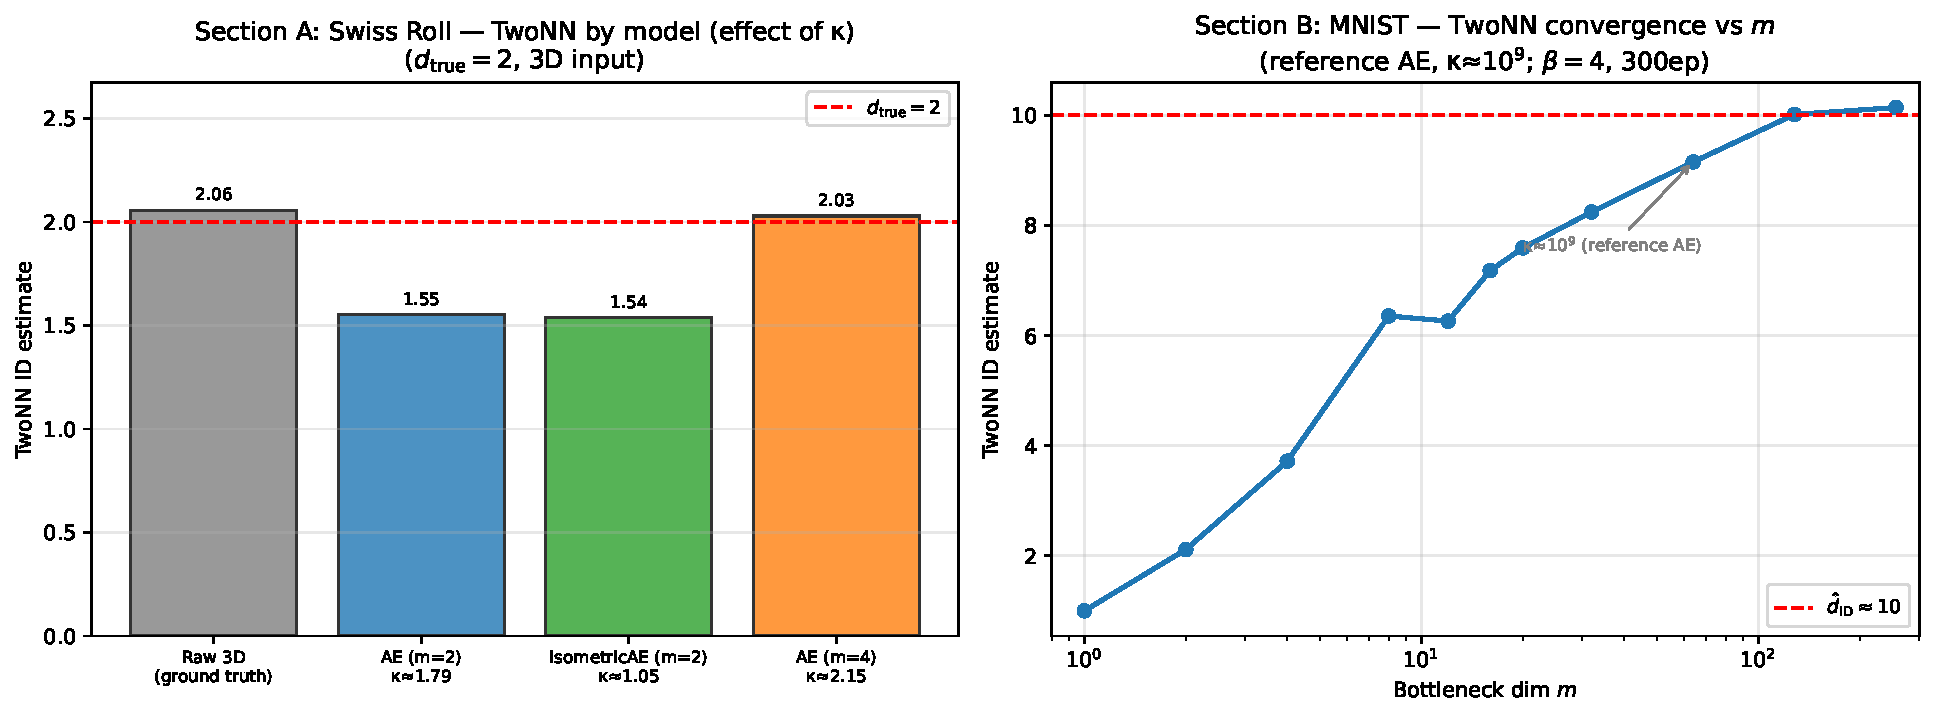
\includegraphics[width=0.95\linewidth]{results/figures/EP_twonn_stability.pdf}
  \caption{Exp-Stab/Exp-Geom: (Left) TwoNN ID on Swiss Roll --- AE and IsometricAE both underestimate at $m=d_\mathrm{true}$; TwoNN recovers at $m=4>d_\mathrm{true}$. (Right) MNIST AE $m$-sweep: TwoNN stabilizes at $m \geq 48$ despite $\kap$ jumping to $37.0$ at $m=128$. Detailed tables in \ref{app:twonn_detail}.}
  \label{fig:ep}
\end{figure}}{}

\subsection{MNIST：有効表現次元の読み取り（主実験，RQ1・RQ2）}\label{sec:exp_mnist}

MNIST データセットを用いて，提案フレームワークの実データへの適用を検証する（主実験）．
MNIST は「実データであり，$\dtrue$は未知であるが$\hat{d}_\mathrm{ID}$を推定できる」
という意味で，フレームワークの現実的な評価環境を提供する．

\subsubsection{AE による内在次元の推定（実験 Exp-Mnist-Base-AE）}

MNIST AE（300 エポック）の結果を表\ref{tab:e4_ae}に示す．

\begin{table}[H]
\centering
\caption{Exp-Mnist-Base: MNIST AE results (300 epochs, $n_\mathrm{train}=20{,}000$; \textbf{single seed 42}).}
\label{tab:e4_ae}
\small
\begin{tabular}{rcccc}
\toprule
$m$ & MSE & TwoNN ID & MLE ID & CKA \\
\midrule
1   & 0.0437 & 1.02  & 1.15  & 0.102 \\
4   & 0.0292 & 3.86  & 4.29  & 0.575 \\
8   & 0.0191 & 6.08  & 6.70  & 0.725 \\
16  & 0.0121 & 7.96  & 8.61  & 0.812 \\
32  & 0.0087 & 8.84  & 9.89  & 0.875 \\
64  & 0.0062 & 9.54  & 11.26 & 0.908 \\
128 & 0.0061 & 9.84  & 11.45 & 0.921 \\
256 & 0.0057 & \textbf{10.02} & \textbf{11.85} & 0.953 \\
\bottomrule
\end{tabular}
\end{table}

$m \geq 64$で TwoNN ID（9.54〜10.02）と MLE ID（11.26〜11.85）が収束し，
MNIST の実効内在次元が概ね$\hat{d}_\mathrm{ID} \approx 10$〜12 の範囲にあることを示す．

\textbf{線形 PCA との比較}：
MNIST（$n = 20{,}000$）に PCA を適用すると，累積寄与率 80\% に 43 次元，
90\% に 86 次元が必要である．
AE（TwoNN $\approx 10$）の推定値と比較して 4〜8 倍大きく，
MNIST の非線形な多様体構造を示している（図\ref{fig:e4_dualaxis}参照）．

\subsubsection{VAE の AU Dynamics と$\mknee$（実験 Exp-Mnist-Base-VAE）}

MNIST VAE（$\beta = 4$，300 エポック）の AU パターンを表\ref{tab:e4_vae}および
図\ref{fig:e4_dualaxis}に示す．

\begin{table}[H]
\centering
\caption{Exp-Mnist-Base: MNIST VAE ($\beta=4$) results (300 epochs; \textbf{single seed 42}). AU increase rate slows at $m=12$ ($\mknee=12$; preliminary, not reproduced in multi-seed runs).}
\label{tab:e4_vae}
\small
\begin{tabular}{rcccc}
\toprule
$m$ & MSE & AU & TwoNN ID & Change in $\rho(m)$ \\
\midrule
1   & 0.0464 & 1  & 1.00 & --- \\
4   & 0.0275 & 4  & 3.72 & normal increase \\
8   & 0.0186 & 8  & 6.36 & normal increase \\
\textbf{12} & 0.0184 & \textbf{8}  & 6.26 & \textbf{sharp drop} $\leftarrow \mknee = 12$ \\
16  & 0.0148 & 11 & 7.18 & low \\
20  & 0.0134 & 13 & 7.59 & low \\
32  & 0.0121 & 15 & 8.25 & low \\
64  & 0.0103 & 29 & 9.16 & gradual \\
128 & 0.0085 & 26 & 10.02 & gradual \\
256 & 0.0072 & 36 & 10.14 & gradual \\
\bottomrule
\end{tabular}
\end{table}

$m = 12$で AU $= 8$（前の$m = 8$と同じ）となり，正規化増加率$\rho(m)$が急落する（$\rho(12) \approx 0$）．
$\tau_{\mathrm{knee}} = 0.25$の閾値をトリガーし，$\mknee = 12$と観測される．

\textbf{注意}：この$\mknee = 12$は単一シード（seed 42）・特定の拡張グリッド
（$m \in \{1,4,8,\ldots,256\}$）での予備的観察であり，
多シード実験（§\ref{sec:exp_multiseed}）では再現されない
（本論文の主要な安定化結果は Exp-Mnist-Dense-300；§\ref{sec:exp_el}）．

\IfFileExists{results/figures/E4_mnist_dualaxis.pdf}{%
\begin{figure}[H]
\centering
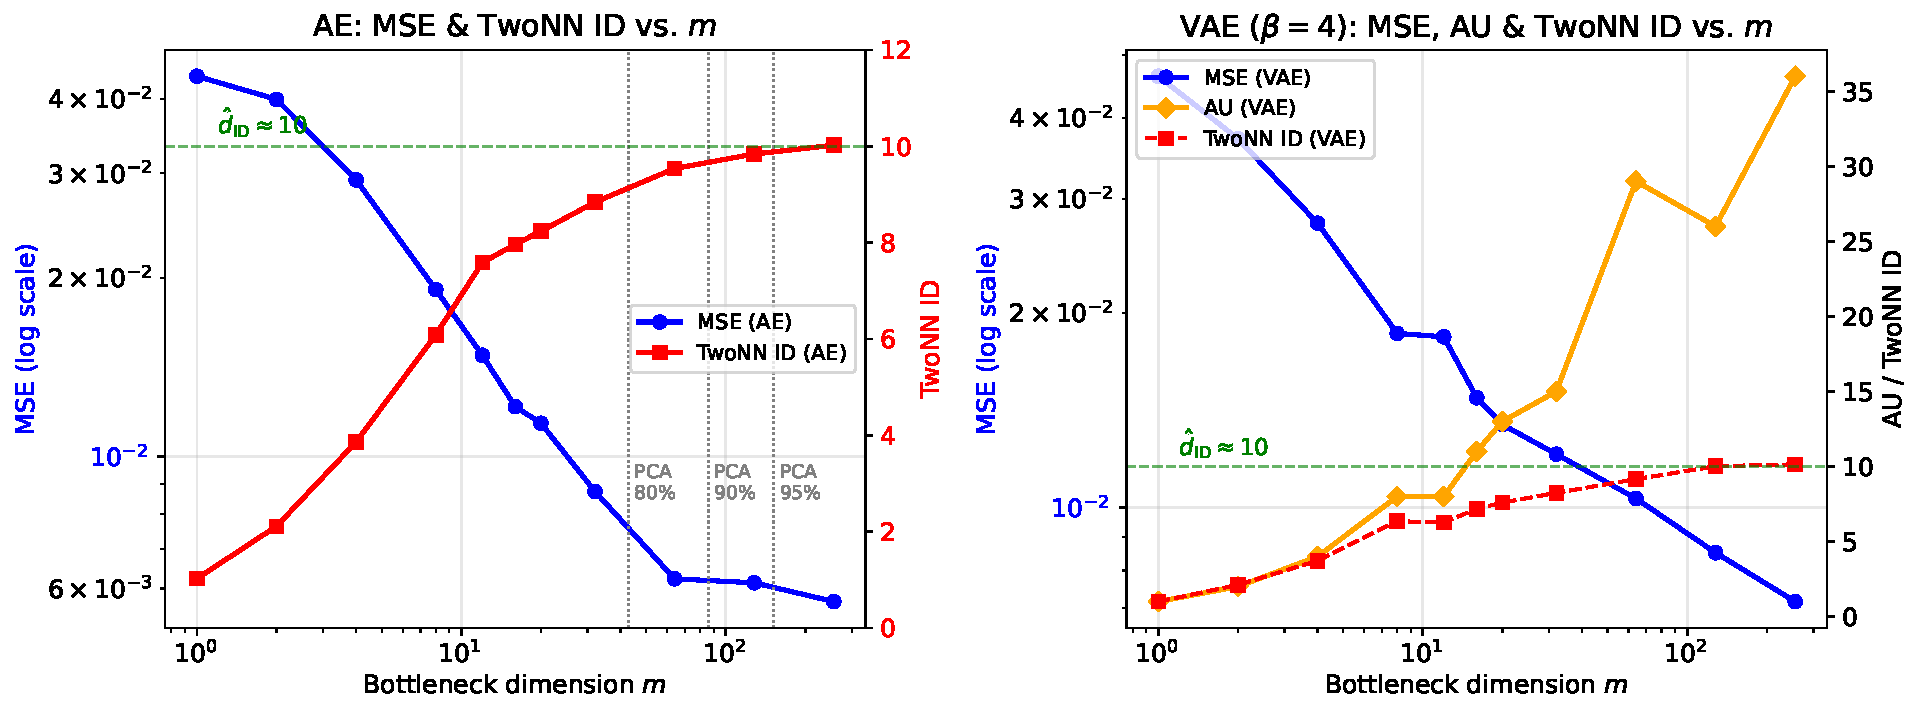
\includegraphics[width=0.95\linewidth]{results/figures/E4_mnist_dualaxis.pdf}
\caption{Exp-Mnist-Base: $m$-dependence of each indicator for MNIST (300 epochs). \textbf{Left (AE)}: MSE (log scale, left axis) and TwoNN ID (right axis). Vertical dotted lines correspond to PCA cumulative variance 80\% (43 dims), 90\% (86 dims), 95\% (152 dims); the difference from the nonlinear AE estimate (TwoNN $\approx 10$) is clear. \textbf{Right (VAE, $\beta=4$)}: MSE (log scale, left axis), AU (right axis), TwoNN ID (right axis, dashed). At $m = 12$ ($\mknee$), the AU increase rate drops sharply (arrow), indicating a heuristic slowdown point; the main stabilized result is $\mknee=10.3\pm0.9$ from Exp-Mnist-Dense-300 (§\ref{sec:exp_el}).}
\label{fig:e4_dualaxis}
\end{figure}}{}%

\subsubsection{既存指標との比較}\label{sec:exp_comparison}

提案指標$\mknee$を，他の代表的なボトルネック次元設計指標と比較する（表\ref{tab:method_comparison}）．

\begin{table}[H]
\centering
\caption{Comparison of bottleneck dimension estimates on MNIST. $\mknee$ entries distinguish sparse-grid and dense-grid conditions.}
\label{tab:method_comparison}
\small
\begin{tabular}{p{4.0cm}cc p{4.5cm}}
\toprule
Method & Estimate & Source & Characteristics / Limitations \\
\midrule
PCA (80\% var.) & 43 & Exp-Mnist-Base-AE & Linear; overestimates nonlinear ID \\
PCA (90\% var.) & 86 & Exp-Mnist-Base-AE & Linear; larger overestimate \\
MSE elbow (AE) & $\approx16$--$20$ & Exp-Mnist-Base-AE & Intuitive; depends on smoothing \\
TwoNN ID (ref.\ AE) & $\approx10$--$12$ & Exp-Mnist-Base-AE & Nonlinear; subject to isometry bias \\
\midrule
$\mknee$ sparse-grid (3 seeds) & $43\pm15$ & Exp-Mnist-Multi-300 & Exploratory; unreliable at sparse grid \\
$\mknee$ \textbf{dense-grid (3 seeds)} & $\boldsymbol{10.3\pm0.9}$ & \textbf{Exp-Mnist-Dense-300} & \textbf{TwoNN-guided local refinement; requires dense grid + multi-seed} \\
\midrule
\multicolumn{4}{p{13.5cm}}{\footnotesize Dense-grid: $m\in\{8,9,\ldots,16,18,\ldots,64\}$ with independent initialization per $(m,\mathrm{seed})$; the dense region was placed around the TwoNN estimate ($\approx10$), so the agreement is a TwoNN-guided refinement, not an independent validation. Sparse-grid $\mknee=43\pm15$ is unreliable as a diagnostic reference.} \\
\bottomrule
\end{tabular}
\end{table}

PCA は線形手法のため非線形な多様体構造を反映できず AE 推定の4倍以上の次元を要求し，
MSE エルボーは平滑な MSE 曲線では肘点の決定が曖昧になりやすい．
$\mknee$は KL ダイナミクスを直接観察する点でこれらと相補的だが，
$\tau$・$\beta$・$m$グリッドへの依存性があり，多指標アプローチでの使用が前提となる．

\subsubsection{多シード検証（実験 Exp-Mnist-Multi-150・Exp-Mnist-Multi-300）}\label{sec:exp_multiseed}
\label{sec:exp_multiseed2}

$\mknee$の統計的信頼性と収束度の影響を評価するため，
MNIST VAE（$\beta = 4$，$m \in \{4,8,12,16,20,32,64\}$）を
3つの乱数シード（42，123，777）で，150 エポック（Exp-Mnist-Multi-150）および
300 エポック（Exp-Mnist-Multi-300）の2条件で学習した．
300 エポック条件の結果を表\ref{tab:e4_300ep_multiseed}に示す
（150 エポック条件の$\mknee$は表\ref{tab:el_mknee}に要約；
AU・TwoNN ID の傾向は 300 エポック条件と同一で，
$m=64$の TwoNN ID は$9.94 \pm 0.08$であった）．

\begin{table}[H]
\centering
\caption{Exp-Mnist-Multi-300: Mean$\pm$std of AU and TwoNN ID for 3 seeds at 300 epochs ($\beta=4$). AU and TwoNN ID are highly consistent, but $\mknee$ still varies.}
\label{tab:e4_300ep_multiseed}
\small
\begin{tabular}{rccl}
\toprule
$m$ & AU (mean$\pm$std) & TwoNN ID (mean$\pm$std) & Note \\
\midrule
 4 & $4.0 \pm 0.0$ & $3.98 \pm 0.14$ & all dims active \\
 8 & $8.0 \pm 0.0$ & $6.67 \pm 0.15$ & \\
12 & $10.0 \pm 0.0$ & $7.41 \pm 0.06$ & \\
16 & $11.7 \pm 0.5$ & $7.95 \pm 0.21$ & AU still increasing \\
20 & $13.3 \pm 0.5$ & $8.37 \pm 0.14$ & \\
32 & $15.7 \pm 0.5$ & $9.07 \pm 0.10$ & \\
64 & $22.3 \pm 0.5$ & $10.03 \pm 0.12$ & converges to $\hat{d}_\mathrm{ID} \approx 10$ \\
\midrule
\multicolumn{4}{l}{$\mknee$（$\tau=0.25$）：シード 42 = 64，シード 123 = 32，シード 777 = 32} \\
\multicolumn{4}{l}{平均$\mknee = 43 \pm 15$（300 エポック）} \\
\bottomrule
\end{tabular}
\end{table}

\IfFileExists{results/figures/E4_300ep_multiseed.pdf}{%
\begin{figure}[H]
  \centering
  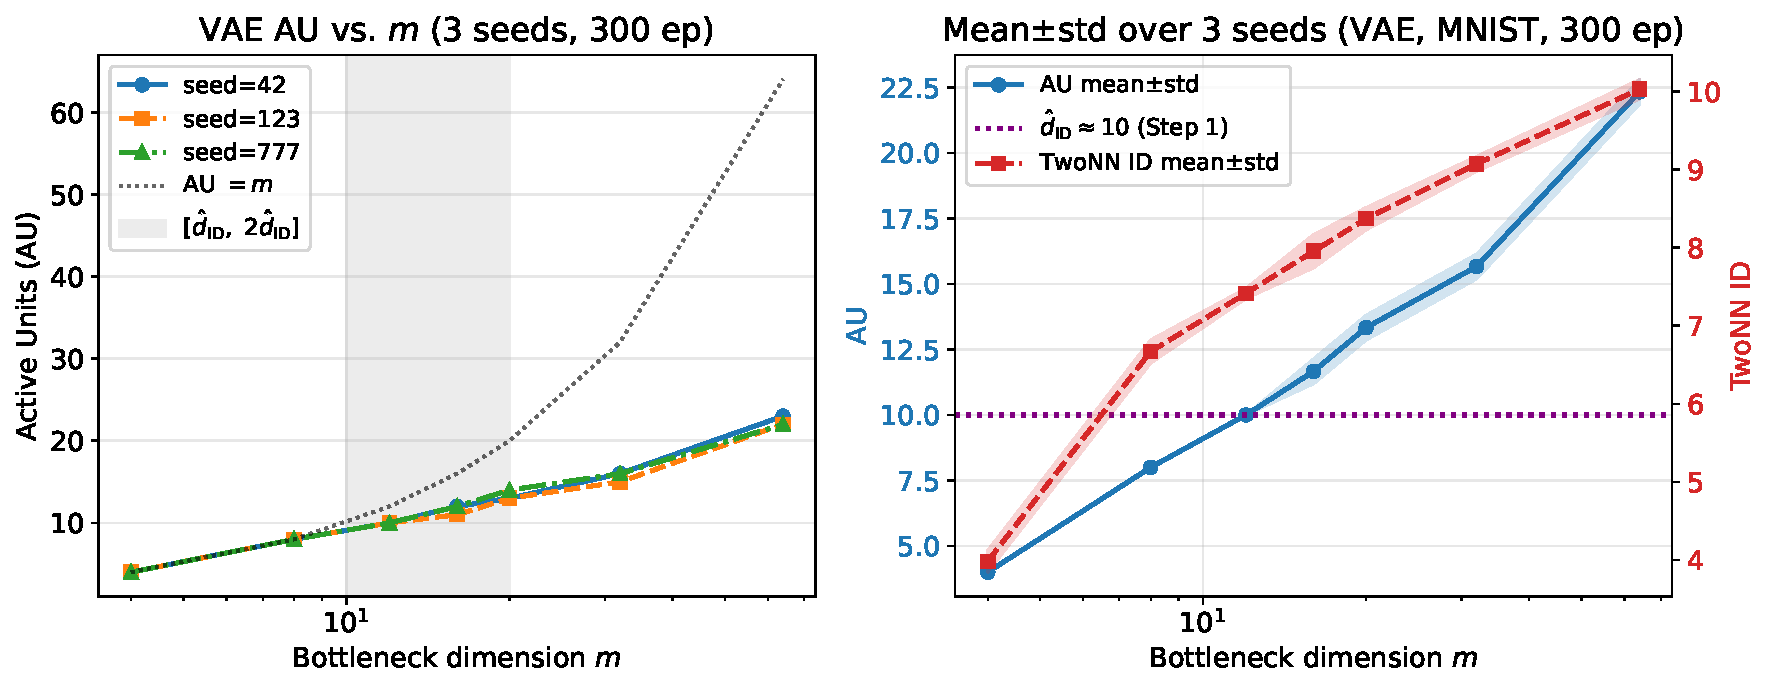
\includegraphics[width=0.9\linewidth]{results/figures/E4_300ep_multiseed.pdf}
  \caption{Exp-Mnist-Multi: AU patterns of MNIST VAE (3 seeds, 300 epochs). Left: AU vs $m$ per seed (dotted lines: $\mknee$); Right: mean$\pm$std band. AU and TwoNN ID bands are very narrow, but $\mknee$ varies between 32 and 64 across seeds.}
  \label{fig:e4_300ep_multiseed}
\end{figure}}{}

\textbf{主要知見}：
AU 値（表\ref{tab:e4_300ep_multiseed}）は両エポック条件とも3シード間で高度に一致し
（$\sigma \leq 0.5$），TwoNN ID も$m = 64$で$10.03 \pm 0.12$（300 エポック）と安定している．
一方，$\mknee$（$\tau=0.25$）は 150 エポックで$53 \pm 15$（シード別 64，32，64），
300 エポックの完全収束下でも$43 \pm 15$（64，32，32）と，いずれも 32〜64 の範囲で変動した．
これは正規化増加率$\rho(m)$が閾値$\tau = 0.25$付近で複数の$m$にわたり微妙に揺動するためであり，
エポック数の延長では解消されない——
\textbf{$\mknee$不安定性の主因は収束不足ではなく$m$グリッドと乱数シードへの依存}である．
Exp-Mnist-Base 拡張実験（単一シード 42）で観測された$\mknee = 12$も本条件では再現されず，
グリッド設計と初期化経路に依存する予備的観察にとどまる（安定化条件は§\ref{sec:exp_el}）．

\subsubsection{線形理論―実験橋渡し（実験 Exp-Mnist-PCA，詳細は\ref{app:twonn_detail}）}\label{sec:exp_em}

MNIST PCA スペクトル（$\lambda_1=5.22, \ldots, \lambda_{10}=1.23$）と定理\ref{thm:linear_vae}を対照すると，
$\tau^2_\mathrm{eff} \approx 0.30$（逆算値）で$d^* \approx 10$となり観測 TwoNN ID と定性的に整合する．
線形設定では鋭い飽和転換が生じるが，非線形 VAE では勾配競合により滑らかな漸増曲線となるため，
$\mknee$の疎グリッドでの不安定性が理論的に裏付けられる（詳細な PCA スペクトル表・理論-実験比較表は\ref{app:twonn_detail}）．
Conv-VAE では非線形デコーダの強力な再構成能力により$\tau^2_\mathrm{eff}$がさらに小さくなり，
AU 飽和に必要な$m$が FC-VAE 比で大幅に増大する（§\ref{sec:disc_convvae}）．

\subsubsection{密グリッドによる TwoNN 誘導型局所精密化（実験 Exp-Mnist-Dense）}\label{sec:exp_el}

$\mknee$の不安定性がどの要因に起因するかを特定するため，
グリッド密度・エポック・シードの3要因を単離した実験を設計した．
Exp-Mnist-Base と Exp-Mnist-Multi では既にエポック因子（150ep vs. 300ep）とシード因子（3シード）が分離されている．
本実験 Exp-Mnist-Dense ではさらにグリッド密度因子を単離する：$m \in \{8,9,10,11,12,13,14,15,16,18,20,24,28,32,40,48,64\}$
（17点，隣接点間隔 1〜16；推定 ID 近傍の$m=8$〜$16$は 1 刻み）で300エポック・3シードで学習した．
\textbf{位置づけの明示}：密領域（$m = 8$〜16）は Stage 1 の TwoNN 推定値
（$\hat{d}_\mathrm{ID} \approx 10$）の近傍に置いたものであり，
候補領域の選択自体が同一フレームワークの TwoNN 推定に依存する．
したがって，後述の$\mknee$と TwoNN ID の一致は\textbf{TwoNN 誘導型の局所精密化}
（TwoNN-guided local refinement）の成功を示すものであり，
TwoNN と独立な相互検証ではない
（事前登録した広域密グリッドや，探索領域の推定と$\mknee$評価を別シード・別データ部分集合で行う
nested validation による独立性の確保は今後の課題である）．

\begin{table}[H]
\centering
\caption{Exp-Mnist-Dense: Comparison of $\mknee$ between dense and sparse grids ($\tau=0.25$, MNIST FC-VAE, $\beta=4$). Consistent with the grid-sensitivity bound of Proposition \ref{thm:mknee_instab}.}
\label{tab:el_mknee}
\small
\begin{tabular}{lccccc}
\toprule
Condition & Max.\ grid interval & seed=42 & seed=123 & seed=777 & Mean$\pm$std \\
\midrule
Sparse, 150ep (Exp-Mnist-Multi-150) & 32 & 64 & 32 & 64 & $53 \pm 15$ \\
Sparse, 300ep (Exp-Mnist-Multi-300) & 32 & 64 & 32 & 32 & $43 \pm 15$ \\
Dense, 300ep (Exp-Mnist-Dense-300) & 16 (step 1, 8--16) & 11 & 9 & 11 & $10.3 \pm 0.9$ \\
\bottomrule
\end{tabular}
\end{table}

\begin{table}[H]
\centering
\caption{Exp-Mnist-Dense: Per-seed AU$(m)$ curves for the full dense grid (300ep, all 3 seeds). The AU curves fluctuate non-monotonically in the transition region ($m=11$--$16$).}
\label{tab:el_au}
\small
\begin{tabular}{l*{17}{c}}
\toprule
$m$ & 8 & 9 & 10 & 11 & 12 & 13 & 14 & 15 & 16 & 18 & 20 & 24 & 28 & 32 & 40 & 48 & 64 \\
\midrule
AU (seed 42)  & 8 & 9 & 10 & 10 & 10 & 10 & 12 & 11 & 14 & 13 & 15 & 14 & 15 & 15 & 18 & 19 & 21 \\
AU (seed 123) & 8 & 8 & 10 & 9  & 11 & 10 & 11 & 13 & 12 & 14 & 13 & 15 & 14 & 17 & 19 & 19 & 21 \\
AU (seed 777) & 8 & 9 & 10 & 10 & 11 & 10 & 11 & 11 & 12 & 12 & 13 & 15 & 16 & 18 & 18 & 20 & 21 \\
\bottomrule
\end{tabular}
\end{table}

\IfFileExists{results/figures/EL_dense_grid_mknee.pdf}{%
\begin{figure}[H]
  \centering
  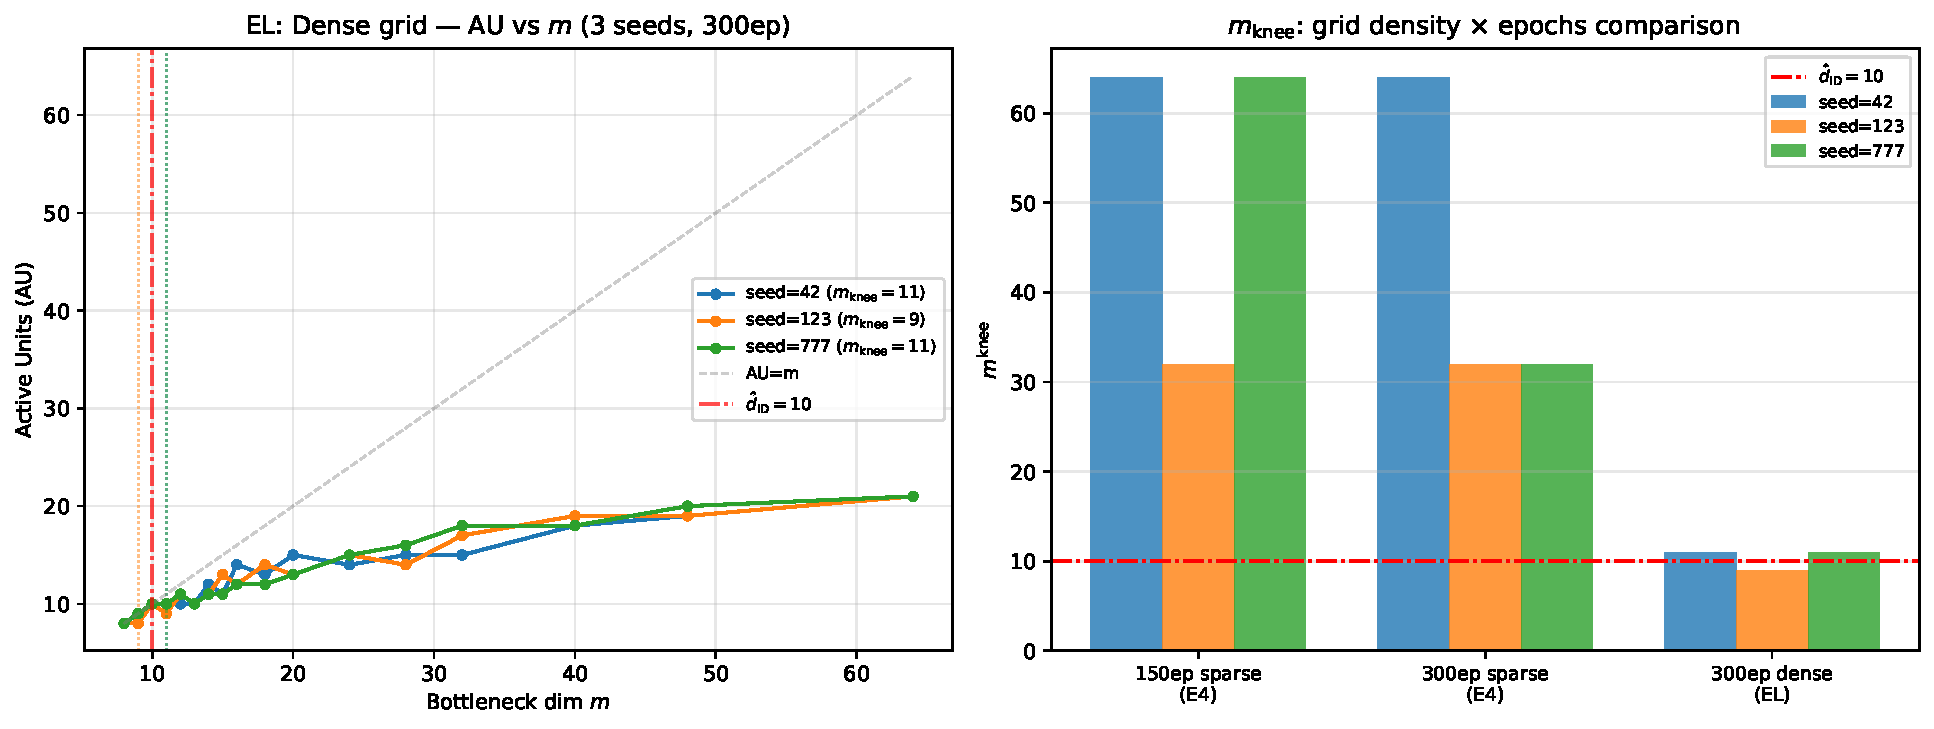
\includegraphics[width=0.95\linewidth]{results/figures/EL_dense_grid_mknee.pdf}
  \caption{Exp-Mnist-Dense: (Left) Dense-grid AU vs $m$ (3 seeds). (Right) Comparison by grid density $\times$ epochs. $\mknee$ variation in the dense grid can be assessed by the upper bound of Proposition~\ref{thm:mknee_instab} (maximum grid interval).}
  \label{fig:el}
\end{figure}}{}

\textbf{3要因の単離}：
表\ref{tab:el_mknee}の3行比較により，
エポック因子（150ep→300ep で$53\pm15$→$43\pm15$；若干の安定化にとどまり主因ではない），
シード因子（同一条件で$\sigma = 15$；二次的因子），
グリッド密度因子（密グリッドで$\mknee = 10.3 \pm 0.9$，シード別 11, 9, 11）が定量的に単離される．
密グリッドの効果は命題\ref{thm:mknee_instab}（理想化モデルでのグリッド設計の重要性）の示唆と
定性的に一致するが，経験的 AU 曲線は非単調な揺動を示すため
（例：表\ref{tab:el_au}で AU$=10$→$10$→$10$→$12$→$11$），
「上界以内に収まった」ではなく
「グリッドを密にすることで経験的$\mknee$の分散が大きく低下した」という観察として述べるのが正確である．
なお TwoNN ID（$\approx 10$）との整合は，密領域を TwoNN 推定値近傍に置いた
TwoNN 誘導型精密化の帰結である点に再度注意する．

\noindent
\textbf{$\tau$法と二階差分法の比較}：
$\mknee$の検出には，本稿で採用している一階差分比率法（$\tau = 0.25$）のほかに，
AU$(m)$曲線の曲率が最大となる点を求める\textbf{二階差分法}（\ref{app:tau_knee}）がある．
Exp-Mnist-Dense 密グリッドデータでの比較結果を表\ref{tab:el_knee_compare}に示す．

\begin{table}[H]
\centering
\caption{Exp-Mnist-Dense: Comparison of $\tau$-method ($\tau=0.25$) and second-difference method (d2) for $\mknee$ detection (dense grid, 300ep, 3 seeds).}
\label{tab:el_knee_compare}
\small
\begin{tabular}{lcccc}
\toprule
Method & seed=42 & seed=123 & seed=777 & Mean$\pm$std \\
\midrule
$\tau$-method ($\tau=0.25$) & 11 & 9  & 11 & $10.3 \pm 0.9$ \\
Second-difference method (d2) & 15 & 28 & 12 & $18.3 \pm 6.8$ \\
\midrule
\multicolumn{5}{l}{Reference: $\hat{d}_\mathrm{ID} \approx 10$ (TwoNN, $m=64$, 3-seed mean)} \\
\bottomrule
\end{tabular}
\end{table}

$\tau$法は平均$10.3 \pm 0.9$と$\hat{d}_\mathrm{ID} \approx 10$に整合し，シード間変動が小さい．
一方，d2 法は AU$(m)$の離散的ノイズに敏感で，seed=123 では$\mknee = 28$と大きく外れた
（AU 曲線の遷移域で AU が 8→10→9→11→10→11→13 と揺動し，二階差分の最大値点が乱れる）．
したがって，\textbf{密グリッド条件での$\mknee$検出には$\tau$法の方が安定}であり，
d2 法は大域的な「肘点」候補を探す補助手段として位置づける（\ref{app:tau_knee}参照）．

なお，MNIST VAE の$\AUsat = 36$（$m=256$）が$\hat{d}_\mathrm{ID} \approx 10$〜12 を大幅に超える点（Manifold Entanglement 仮説）と，
学習ダイナミクスの2フェーズパターン（Exp-Mnist-Dyn）は，いずれも単一シード・予備的観察であり，
多シード検証は今後の課題として残す（§\ref{sec:disc_incidental}参照）．

\subsection{Fashion-MNIST への適用（実験 Exp-Fashion，探索的補助証拠）}\label{sec:exp_fashion}

Fashion-MNIST（衣類 10 クラス，28×28；100 エポック，\textbf{単一シード 42}）は，
多シード検証を欠くため\textbf{外部検証ではなく探索的補助証拠}として位置づけ，
結果表・図の詳細は\ref{app:fashion}（表\ref{tab:ef}，図\ref{fig:ef}）に移す．
要点のみ述べると：AE では TwoNN ID が$m \geq 32$で$\approx 9.4$に収束し
$\hat{d}_\mathrm{ID} \approx 9$〜10 が示唆される；
VAE（$\beta = 4$）では$\mknee = 12$（$\tau_{\mathrm{knee}} = 0.25$）が観測されたが
単一シードの探索的観察であり，MNIST 3シード実験と同水準の再現性は主張しない．
Fashion-MNIST の多シード再現は今後の課題である
（なお多シードでの実データ検証としては Exp-Real-Geom が Fashion-MNIST を含む；
§\ref{sec:exp_real_geom}）．

\subsection{畳み込みアーキテクチャへの拡張（実験 Exp-Conv-AE）}\label{sec:exp_conv}

全結合型に限定した場合の一般化可能性への懸念に対し，
畳み込み型 AE/VAE（Conv-AE/VAE）を MNIST に適用した（実験 Exp-Conv-AE；
100 エポック，$m \in \{4, 8, 12, 16, 20, 32, 64\}$，\textbf{単一シード 42}．
アーキテクチャ詳細と結果表は\ref{app:fashion}，表\ref{tab:eg}）．
\textbf{Conv-AE の TwoNN ID}は$m = 64$で$11.29$に収束し FC-AE の推定値（$\approx 10$）と
整合する（誤差$\approx 10\%$以内）——アーキテクチャによらず TwoNN 推定値が一貫する
（本研究条件下での経験的観測）．
一方 \textbf{Conv-VAE}は$m \leq 32$で AU $= m$（飽和なし）であり，
100 エポックでは KL 正則化による次元抑制が機能せず，
$\mknee$の信頼ある検出にはより多くのエポック数が必要である．

\subsubsection{Conv-VAE での AU 飽和遅延：固定$\beta$・KL アニーリング比較（実験 Exp-Conv-Fix・Exp-Conv-Ann）}
\label{sec:exp_conv_300ep}

Exp-Conv-AE の収束不足を受け，300ep・3シード（Exp-Conv-Fix）および KL サイクリックアニーリング（Exp-Conv-Ann）で検証した
（表\ref{tab:eh_conv_vae}）．

\begin{table}[H]
\centering
\caption{Exp-Conv-Fix and Exp-Conv-Ann: Comparison of AU for MNIST Conv-VAE (300ep, mean$\pm$std over 3 seeds). FC-VAE (Exp-Mnist-Multi-300) slows down by $m=32$ (AU$=15.7$), while Conv-VAE shows AU$=m$ (no saturation) under both fixed-$\beta$ and annealing at $m \leq 32$.}
\label{tab:eh_conv_vae}
\small
\begin{tabular}{r ccc cc}
\toprule
 & \multicolumn{2}{c}{\shortstack{Conv-VAE fixed-$\beta$\\(Exp-Conv-Fix)}} & \multicolumn{1}{c}{\shortstack{Conv-VAE annealing\\(Exp-Conv-Ann)}} & \multicolumn{2}{c}{\shortstack{FC-VAE\\(Exp-Mnist-Multi-300)}} \\
$m$ & AU & TwoNN ID & AU & AU & TwoNN ID \\
\midrule
 4 & $4.0\pm0.0$ & $3.97\pm0.08$ & $4.0\pm0.0$ & $4.0$ & $3.98$ \\
12 & $12.0\pm0.0$ & $8.14\pm0.09$ & $12.0\pm0.0$ & $10.0$ & $7.41$ \\
32 & $32.0\pm0.0$ & $11.43\pm0.08$ & $32.0\pm0.0$ & $15.7$ & $9.07$ \\
64 & $54.3\pm0.5$ & $13.10\pm0.05$ & $64.0\pm0.0$ & $22.3$ & $10.03$ \\
\midrule
\multicolumn{6}{l}{$\mknee$：Conv-VAE（両条件）全シード=64（グリッド上限）；FC-VAE=$43\pm15$（32〜64）} \\
\bottomrule
\end{tabular}
\end{table}

Conv-VAE は固定$\beta=4$・サイクリックアニーリングいずれでも$m \leq 32$で AU$=m$（飽和なし）であり，
FC-VAE との乖離が明確である（§\ref{sec:disc_convvae}で理論的考察）．
AU$\approx m$は「KL 正則化が未機能」のシグナルであり，この状態では TwoNN ID も膨張する
（Conv-VAE $m=64$: $13.10$，FC-VAE: $10.03$）．
\textbf{$m \leq 64$のグリッドでは AU 飽和の観察が不可能}であり，$m$ 範囲の拡張が必要である．

%% ===================================================================
\subsection{Conv-VAE 拡張$m$グリッド実験（実験 Exp-Conv-M256・Exp-Conv-M512）}\label{sec:exp_en}

Exp-Conv-Fix・Exp-Conv-Ann（§\ref{sec:exp_conv_300ep}）で$m \leq 64$では AU 飽和が観測されなかったことを受け，
$m$グリッドを 256（実験 Exp-Conv-M256）および 512（実験 Exp-Conv-M512）まで拡張した．
§\ref{sec:disc_convvae}で論じる$\tau^2_\mathrm{eff}$の低下仮説のもとでは，
Conv-VAE の$d^*(\beta)$は FC-VAE（$\approx 10$）より大幅に大きいため，
$m>64$の領域で AU 増加の鈍化が現れると予測される．

\textbf{実験設定}（Exp-Conv-M256）：
Exp-Conv-Ann と同一の Conv-VAE アーキテクチャ（$28\times28$ MNIST，2層 Conv エンコーダ・
2層 ConvTranspose デコーダ，KL サイクリックアニーリング$\beta_\mathrm{max}=4$，3サイクル，
150 エポック，seeds$\in\{42,123,777\}$）を用い，
$m \in \{4, 8, 16, 32, 64, 96, 128, 192, 256\}$（9点）を検証した．

\begin{table}[H]
\centering
\caption{Exp-Conv-M256: Conv-VAE extended $m$ grid (KL annealing, 150 epochs, mean$\pm$std, 3 seeds). AU$=m$ for $m \leq 64$; AU$<m$ begins at $m \geq 96$. FC-VAE reference (Exp-Mnist-Multi-300, $m=64$): AU$=22.3\pm0.5$.}
\label{tab:en}
\small
\begin{tabular}{rccc}
\toprule
$m$ & AU (mean$\pm$std) & TwoNN ID (mean$\pm$std) & Note \\
\midrule
  4 & $4.0\pm0.0$   & $3.84\pm0.11$ & all dims active \\
  8 & $8.0\pm0.0$   & $6.64\pm0.11$ & \\
 16 & $16.0\pm0.0$  & $8.76\pm0.05$ & \\
 32 & $32.0\pm0.0$  & $10.46\pm0.13$ & \\
 64 & $64.0\pm0.0$  & $13.29\pm0.12$ & same as Exp-Conv-Ann (no saturation) \\
 96 & $\mathbf{90.7\pm1.2}$  & $14.30\pm0.22$ & \textbf{AU$<m$ onset} (FC-VAE $\hat{d}_\mathrm{ID} \approx 9\times$) \\
128 & $111.7\pm2.6$ & $14.69\pm0.13$ & \\
192 & $159.0\pm4.3$ & $15.89\pm0.27$ & \\
256 & $241.3\pm2.9$ & $16.58\pm0.16$ & \\
\midrule
\multicolumn{4}{l}{$\mknee$（$\tau=0.25$）：全シード=256（検証範囲内に knee なし）} \\
\multicolumn{4}{l}{FC-VAE reference (Exp-Mnist-Multi-300, $m=64$): AU$=22.3\pm0.5$, TwoNN ID$=10.03\pm0.12$} \\
\bottomrule
\end{tabular}
\end{table}

\IfFileExists{results/figures/EN_conv_vae_extended_m.pdf}{%
\begin{figure}[H]
  \centering
  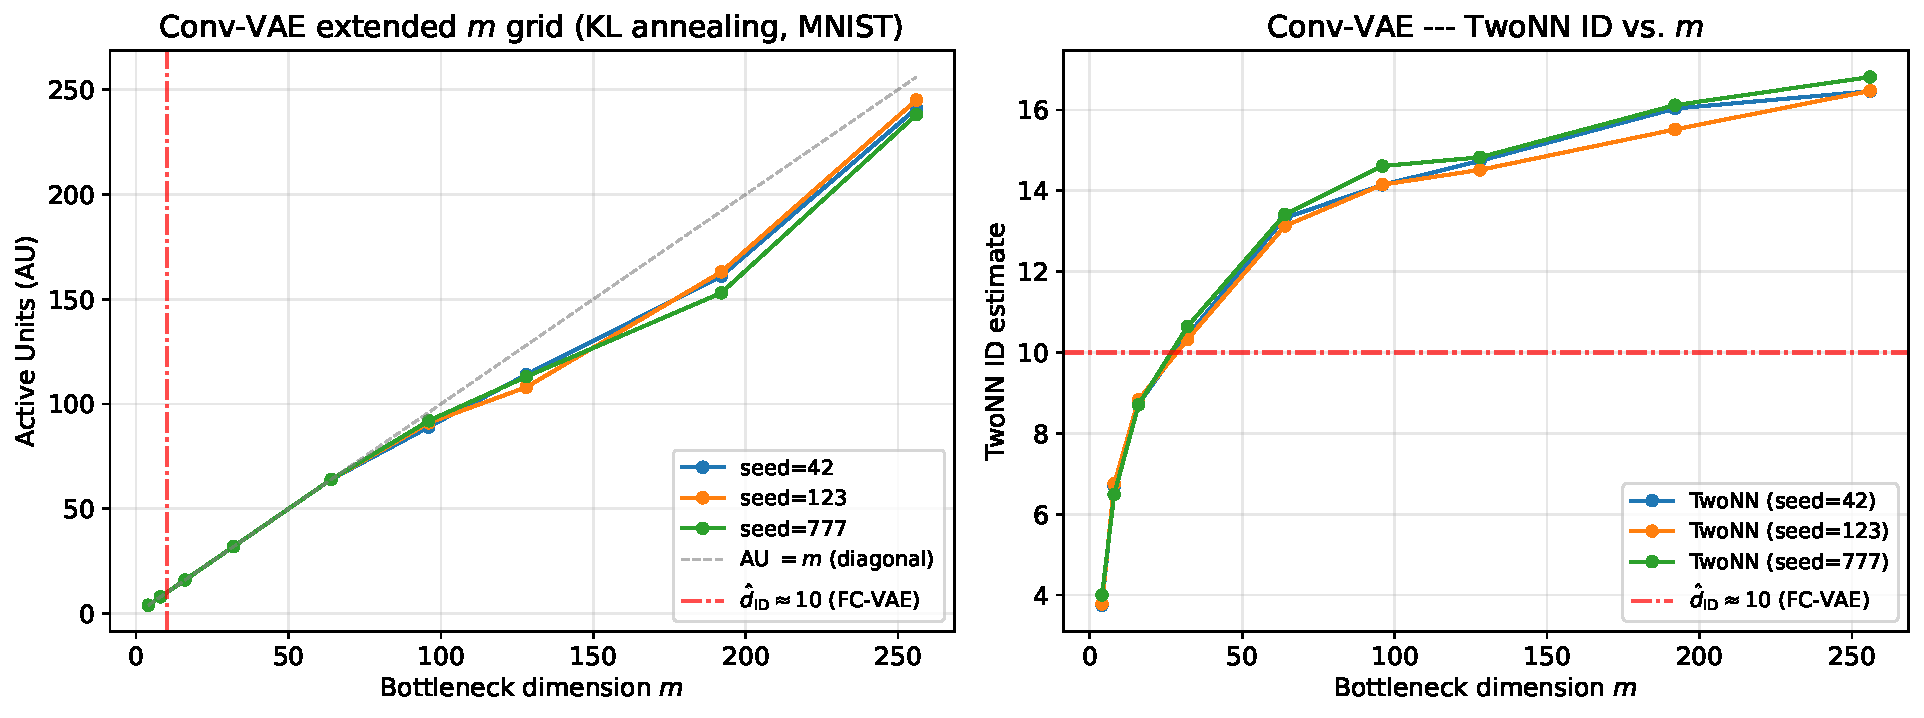
\includegraphics[width=0.95\linewidth]{results/figures/EN_conv_vae_extended_m.pdf}
  \caption{Exp-Conv-M256: Conv-VAE extended $m$ grid ($m\in[4,256]$, KL annealing, 3 seeds). AU vs $m$ (left) and TwoNN ID vs $m$ (right). Diagonal line (AU$=m$) and FC-VAE reference $\hat{d}_\mathrm{ID} \approx 10$ (red) are shown. AU$=m$ continues at $m \leq 64$ but deviates from the diagonal at $m \geq 96$, confirming qualitative water-filling behavior in Conv-VAE.}
  \label{fig:en}
\end{figure}}{}

\textbf{実験 Exp-Conv-M256 の主要知見}：
$m \leq 64$では AU$=m$が全3シードで一致し（FC-VAE の$m=64$: AU$=22.3$と対照的），
$m = 96$で初めて AU$=90.7\pm1.2 < m$と飽和傾向が現れるが，
$m=256$でも活性率 94.3\%と高く，$\mknee$は全シードでグリッド端（256）に留まった．
Conv-VAE の$d^*(\beta)$は FC-VAE（$\approx 10$）より大幅に大きい（$> 256$）ことを示す
（$\tau^2_\mathrm{eff}$理論との対応は§\ref{sec:disc_convvae}）．

\textbf{$m=256$超への拡張（実験 Exp-Conv-M512，詳細は\ref{app:convvae_natimg}）}：
$m \in \{384, 512\}$まで拡張しても AU$\approx m$（全次元活性）が全3シードで維持され，
$\mknee$はグリッド端 512 に張り付いたままであった（\ref{app:convvae_natimg}，表\ref{tab:en_ext}参照）．
MNIST Conv-VAE の$d^*(\beta)$が$m=512$を超えることを示しており，
§\ref{sec:disc_convvae}の$\tau^2_\mathrm{eff}$理論予測と整合する．
次節では$\beta_{\max}$を強化して AU 飽和を人為的に誘発できることを示す．

%% ===================================================================
\subsection{高$\beta$による Conv-VAE AU 飽和の人為的誘発（実験 Exp-ConvV-HiBeta）}\label{sec:exp_hibeta}

§\ref{sec:disc_convvae}の$\tau^2_\mathrm{eff}$仮説（強力デコーダが AU 飽和を高次元側に押しやる）の
検証として，$\beta_{\max}$を$4 \to \{10, 20\}$に増大させ，MNIST Conv-VAE での
AU 飽和プラトーが誘発されるかを確認した．

\textbf{実験設定}：Exp-Conv-M256 と同一アーキテクチャ・KL サイクリックアニーリング（3サイクル）を使用し，
$\beta_{\max} \in \{10, 20\}$，$m \in \{16, 32, 64, 96, 128, 192, 256\}$，
seed=42，150 エポックで学習した（比較用として Exp-Conv-M256 の$\beta_{\max}=4$ seed=42 結果を再掲する）．

\begin{table}[H]
\centering
\caption{Exp-ConvV-HiBeta: Comparison of MNIST Conv-VAE AU at $\beta_\mathrm{max} \in \{4, 10, 20\}$ (\textbf{single seed 42}, 150ep, KL cyclic annealing; exploratory). Higher $\beta_\mathrm{max}$ induces AU saturation at lower dimensions.}
\label{tab:hibeta}
\small
\begin{tabular}{r ccc}
\toprule
$m$ & $\beta_{\max}=4$ (Exp-Conv-M256) & $\beta_{\max}=10$ & $\beta_{\max}=20$ \\
\midrule
 16  & 16  (100\%)& 16 (100\%) & 16 (100\%) \\
 32  & 32  (100\%)& 32 (100\%) & 27 (84\%)  \\
 64  & 64  (100\%)& 54 (84\%)  & 42 (66\%)  \\
 96  & 89  (93\%) & 65 (68\%)  & 47 (49\%)  \\
128  & 114 (89\%) & 69 (54\%)  & 53 (41\%)  \\
192  & 161 (84\%) & 79 (41\%)  & 60 (31\%)  \\
256  & 241 (94\%) & 93 (36\%)  & 66 (26\%)  \\
\midrule
$\mknee$ ($\tau=0.25$) & 512 (grid boundary, unidentified) & $\approx 128$ & $\approx 96$ \\
\bottomrule
\end{tabular}
\end{table}

\textbf{Exp-ConvV-HiBeta の知見}（表\ref{tab:hibeta}）：
$\beta_{\max}=4$では$m \leq 64$で AU$=m$（100\%活性）が続くのに対し，
$\beta_{\max}=10$では$m=64$で AU$=54$（84\%），$m=128$で AU$=69$（54\%），$m=256$で AU$=93$（36\%）と
明確な AU 飽和傾向が現れ，$\mknee \approx 128$（$\tau=0.25$）が同定された．
さらに$\beta_{\max}=20$では$m=32$で AU$=27$（84\%），$m=64$で AU$=42$（66\%）と
より低次元側で飽和が生じ，$\mknee \approx 96$が観測された．
これは§\ref{sec:disc_convvae}の$\tau^2_\mathrm{eff}$仮説の予測に直接整合する：
$\beta$を増大させると$d^*(\beta) = |\{j: \lambda_j > \beta\tau^2_\mathrm{eff}\}|$が小さい値に移動し，
AU 飽和がより低次元側に現れる．
\textbf{この結果は，MNIST Conv-VAE での AU 飽和未観測が「フレームワークの適用限界」ではなく，
$\beta_{\max}=4$ という設定ではデコーダ容量に比して正則化が不足し$d^*(\beta) \gg 256$となっていたことに起因する}
という解釈と整合する．AU/$\mknee$診断フレームワークの Conv-VAE への適用には，
データ・アーキテクチャに合わせた$\beta$の適切な設定が必要である
（本実験は単一シードの探索的観察であり，多シード再現は今後の課題である）．

\IfFileExists{results/figures/Exp_ConvV_HiBeta.pdf}{%
\begin{figure}[H]
\centering
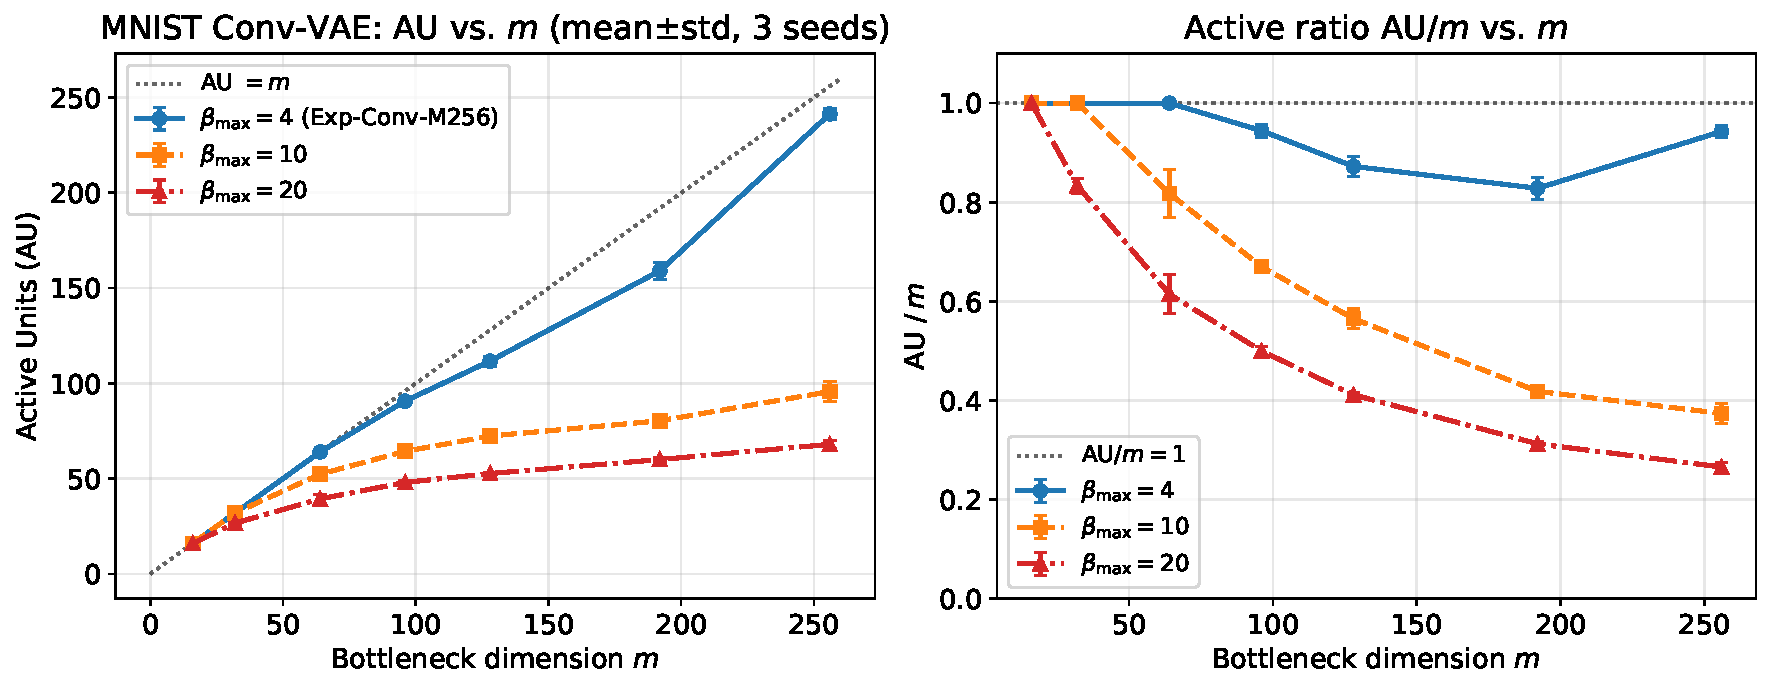
\includegraphics[width=0.9\linewidth]{results/figures/Exp_ConvV_HiBeta.pdf}
\caption{Exp-ConvV-HiBeta: Comparison of MNIST Conv-VAE AU vs $m$ (left) and activation rate AU/$m$ (right) for $\beta_{\max} \in \{4, 10, 20\}$. Increasing $\beta_{\max}$ shifts AU saturation to lower dimensions, demonstrating the $\beta$-dependence of $d^*(\beta)$.}
\label{fig:hibeta}
\end{figure}
}{}

%% ===================================================================
\subsection{自然画像への適用：CIFAR-10・SVHN（実験 Exp-Nat-Cifar・Exp-Nat-SVHN）}\label{sec:exp_natural}

より複雑な自然画像データセット（CIFAR-10\cite{krizhevsky2009learning}，
SVHN\cite{netzer2011reading}）に対して本フレームワークを適用し，
Pope ら\cite{pope2021intrinsic}の内在次元推定との比較を行った．

\textbf{実験設定}（Exp-Nat-Cifar：CIFAR-10，Exp-Nat-SVHN：SVHN）：
3層 Conv エンコーダ（$3{\to}32{\to}64{\to}128$，$k=4$，stride 2）＋
3層 ConvTranspose デコーダの Conv-VAE（入力$32 \times 32 \times 3$）を用い，
$n_{\mathrm{train}} = 20{,}000$，150 エポック，
KL サイクリックアニーリング（$\beta_{\max}=4$，3サイクル），
$m \in \{16, 32, 64, 128, 256\}$，3シード（42, 123, 777）で学習した．

\begin{table}[H]
\centering
\caption{Exp-Nat-Cifar and Exp-Nat-SVHN: Conv-VAE results for CIFAR-10 (left) and SVHN (right) (mean$\pm$std, 3 seeds; KL cyclic annealing, 150 epochs, 3 cycles). At $m=64$, CIFAR-10 latent TwoNN ID converges to the raw-data value ($\approx25$), consistent with Pope et al.\ \cite{pope2021intrinsic} ($d_\mathrm{ID} \approx 26$).}
\label{tab:ei_ej}
\small
\begin{tabular}{r cc | cc}
\toprule
 & \multicolumn{2}{c|}{CIFAR-10 (Exp-Nat-Cifar)} & \multicolumn{2}{c}{SVHN (Exp-Nat-SVHN)} \\
$m$ & AU (mean$\pm$std) & TwoNN ID (mean$\pm$std) & AU (mean$\pm$std) & TwoNN ID (mean$\pm$std) \\
\midrule
 16  & $16.0\pm0.0$ & $13.12\pm0.12$ & $16.0\pm0.0$ & $11.30\pm0.12$ \\
 32  & $32.0\pm0.0$ & $19.26\pm0.23$ & $32.0\pm0.0$ & $15.08\pm0.08$ \\
 64  & $64.0\pm0.0$ & $\mathbf{25.21\pm0.41}$ & $64.0\pm0.0$ & $19.97\pm0.12$ \\
128  & $128.0\pm0.0$ & $28.83\pm0.41$ & $125.3\pm0.5$ & $24.60\pm0.36$ \\
256  & $256.0\pm0.0$ & $30.91\pm0.64$ & $206.7\pm1.2$ & $27.08\pm0.34$ \\
\midrule
\multicolumn{3}{l|}{Raw TwoNN=25.20, MLE=26.56 ($\approx$ Pope et al.\ estimate of 26)} & \multicolumn{2}{l}{Raw TwoNN=10.09, MLE=18.85} \\
\multicolumn{3}{l|}{$\mknee$ ($\tau=0.25$): all seeds=256 (no knee in range)} & \multicolumn{2}{l}{$\mknee$: all seeds=256 (no knee in range)} \\
\bottomrule
\end{tabular}
\end{table}

\IfFileExists{results/figures/EI_cifar10_conv_vae.pdf}{%
\begin{figure}[H]
  \centering
  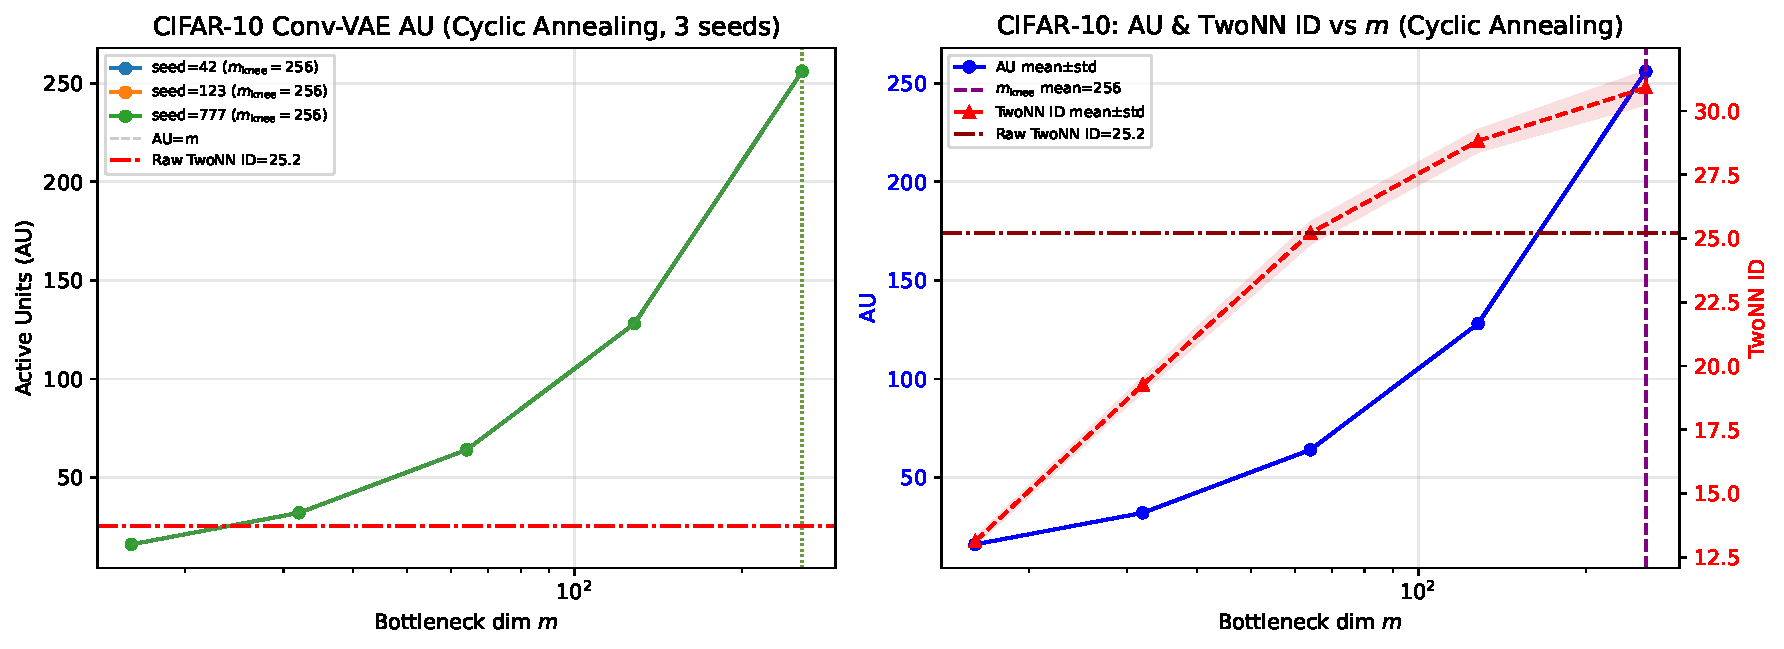
\includegraphics[width=0.95\linewidth]{results/figures/EI_cifar10_conv_vae.pdf}
  \caption{Exp-Nat-Cifar: $m$-dependence of AU and TwoNN ID for CIFAR-10 Conv-VAE (KL cyclic annealing, 3 seeds). TwoNN ID shows convergence consistent with Pope et al.\cite{pope2021intrinsic} ($d_\mathrm{ID} \approx 26$).}
  \label{fig:ei}
\end{figure}}{}

\IfFileExists{results/figures/EJ_svhn_conv_vae.pdf}{%
\begin{figure}[H]
  \centering
  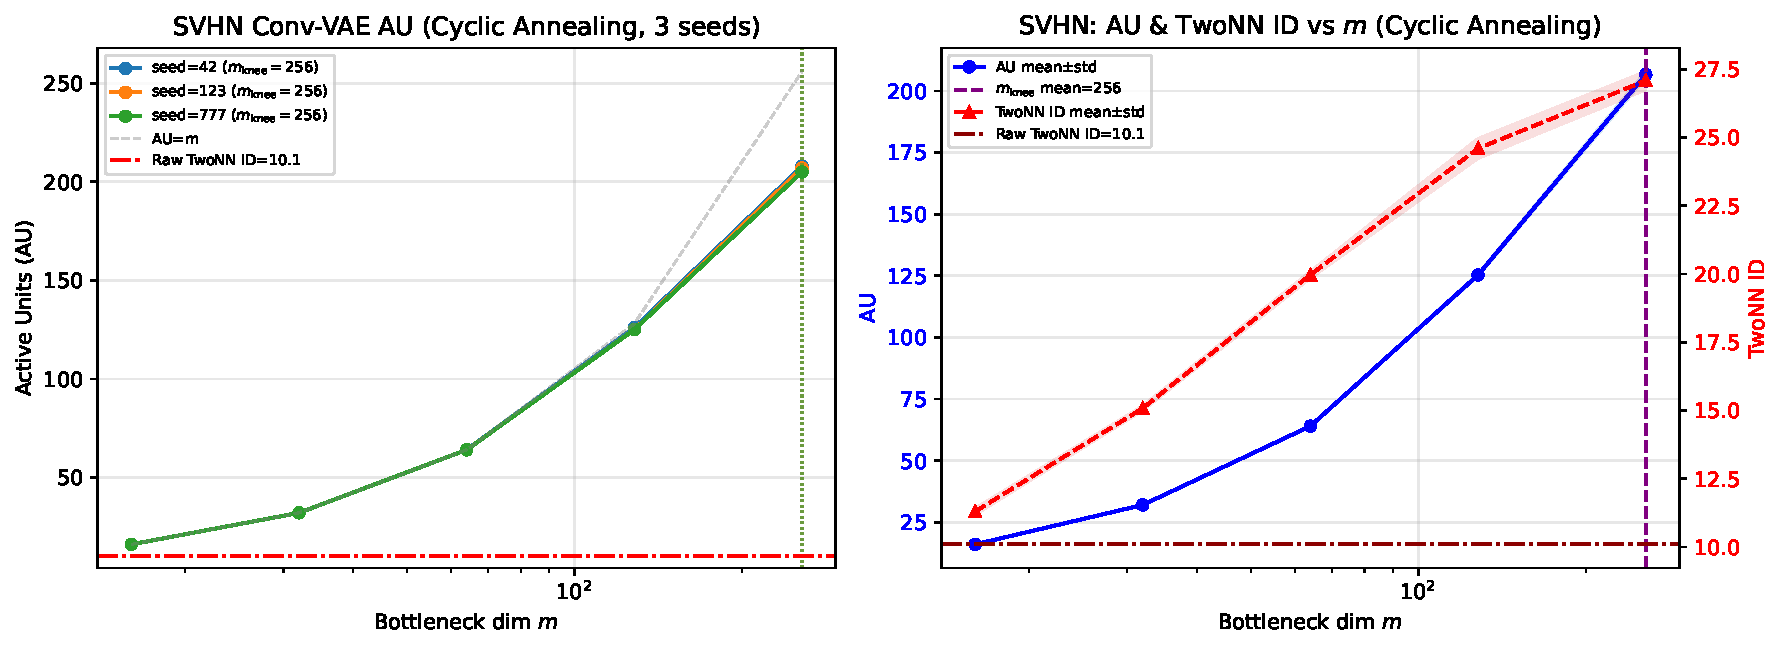
\includegraphics[width=0.95\linewidth]{results/figures/EJ_svhn_conv_vae.pdf}
  \caption{Exp-Nat-SVHN: $m$-dependence of AU and TwoNN ID for SVHN Conv-VAE (KL cyclic annealing, 3 seeds).}
  \label{fig:ej}
\end{figure}}{}

本実験の主眼は TwoNN ID が適切なボトルネック範囲で Pope らの報告値と同程度のスケールを示すかの
確認に限定される（AU/$\mknee$ 側の安定同定は自然画像では未達であり，本実験は適用境界を定める）．
主要な知見は次の2点である（表\ref{tab:ei_ej}）．
\textbf{CIFAR-10}：$m=64$での潜在 TwoNN ID$=25.21\pm0.41$（3シード）は
生データ TwoNN ID（25.20）および Pope ら\cite{pope2021intrinsic}の報告値（$\approx 26$）と
同程度のスケールを示すが，$m=128$以上では 28.8〜30.9 へ上昇する——
TwoNN の数値的整合は$m \approx 2\hat{d}_\mathrm{ID}$程度の範囲に限られる．
AU は$m \leq 256$で AU$=m$（飽和なし，$\mknee$は全シードでグリッド端）であり，
フレームワーク全体の自然画像への汎化を主張するものではない．
\textbf{SVHN}：$m \geq 128$で AU$<m$となるが AU 飽和プラトーには至らず，
潜在 TwoNN ID（$m=256$で 27.08）は生データ TwoNN（10.09）から大きく乖離する——
AU が全次元を使用する条件では潜在空間の幾何的歪みにより ID が過大推定されうることを示す
適用限界の一例である．

\subsection{CIFAR-10 Conv-VAE における AU 飽和条件の探索（実験 Exp-NatImg-AU，詳細は\ref{app:convvae_natimg}）}\label{sec:exp_natimg_au}

本節と§\ref{sec:exp_natimg_sweep}は「適用境界の定量化」実験である——
AU/$\mknee$ 安定同定の失敗を報告するのではなく，
どの条件下で AU 診断が困難になるかの境界条件を体系的に特定する．
Exp-Nat-Cifar（$\beta_{\max}=4$）で AU 飽和が観測されなかった要因
（$\beta$不足・学習不足・容量不足）を切り分けるため，
$\beta_{\max} \in \{10, 20, 40\}$と2種類のアーキテクチャ（Standard/Deep）を系統的に変化させた
（CIFAR-10，$m \in [32, 384]$，KL サイクリックアニーリング，200 エポック，\textbf{単一シード 42}；
実験設定・AU 表・図の詳細は\ref{app:convvae_natimg}，表\ref{tab:natimg_au}）．

\textbf{主要な観察}：
（1）$\beta_{\max}$増大は次元抑制をもたらす（$\beta_{\max}=40$・Deep：$m=384$で AU$=208$，利用率 54\%）が，
いずれの条件でも AU$(m)$は単調増加を続け，飽和プラトーは現れない（$\mknee=384$：全条件でグリッド端）．
（2）潜在 TwoNN ID はピクセル空間 TwoNN（25.30）を超えて増加し続け
（Arch-A・$\beta_{\max}=10$：$m=256$で 29.2），
AU が全次元を利用する状況では潜在幾何の歪みにより ID が過大推定される傾向を示す．
（3）定理\ref{thm:linear_vae}の観点では，強力な Conv デコーダにより実効ノイズ分散$\tau^2_\mathrm{eff}$が
MNIST より大幅に小さく，$\beta$の増大だけでは活性化条件$\lambda_j > \beta\tau^2_\mathrm{eff}$を
反転させることが難しい．
以上から，AU 飽和による$\mknee$同定には（a）$m \gg 2\hat{d}_\mathrm{ID}$の広域グリッド探索，
または（b）デコーダ容量を制限した設定が必要条件であることが特定された（§\ref{sec:disc_convvae}）．
次節の拡張スイープでこの境界条件をさらに定量化する．

%% ===================================================================
\subsection{実データ幾何比較実験：TwoNN 安定性条件の実証（RQ2・RQ3）}\label{sec:exp_real_geom}

本実験（Exp-Real-Geom）は命題\ref{thm:twonn_stability}の実験的検証として，
MNIST・Fashion-MNIST において \textbf{等長性を系統的に変化させた4種類のモデル}を
複数の$m$値でスイープし，TwoNN・MLE・$\kap$・Trustworthiness・kNN overlap を比較する．

\subsubsection*{実験設定（Exp-Real-Geom）}

\textbf{モデル}：以下の4種類を比較する．
\begin{description}
  \item[通常 AE] ヤコビアン正則化なし（$\kap \approx 10^2$〜$10^7$；$m$の増大とともに増大，表\ref{tab:real_geom_mnist}）
  \item[IsometricAE] デコーダヤコビアン正則化（$\kap \approx 1.1$〜1.4；Kato ら\cite{kato2020rdae}）
  \item[CAE] エンコーダ側収縮正則化（$\kap$中程度；Rifai ら\cite{rifai2011cae}）
  \item[DAE] 入力ノイズ正則化（ノイズスケール$\sigma=0.1$；Alain ら\cite{alain2014dae}）
\end{description}

\textbf{$m$スイープ}：$m \in \{d, 2d, 3d, 5d, 10d\}$
（$d = \hat{d}_\mathrm{ID}$を MNIST では 10，Fashion-MNIST では 9 と設定；
すなわち$m \in \{10, 20, 30, 50, 100\}$および$m \in \{9, 18, 27, 45, 90\}$）．

\textbf{測定指標}：TwoNN（$k=2$），MLE（$k=10$），$\kap$（デコーダヤコビアン条件数），
Trustworthiness（$k=10$），kNN overlap（kNN 近傍保持率，$k=10$）．

\textbf{データ・学習}：MNIST・Fashion-MNIST，学習サンプル 20,000，
シード$\{42, 123, 777\}$（3シード），300エポック，隠れ層$[512, 256]$，Adam（lr$=10^{-3}$）．

\subsubsection*{実験結果（Exp-Real-Geom）}

主要な結果の要約を表\ref{tab:real_geom_summary}に示す（全$m$・全指標の詳細表は
\ref{app:twonn_detail}，表\ref{tab:real_geom_mnist}）．

\begin{table}[H]
\centering
\caption{Exp-Real-Geom (summary): MNIST four-model comparison (mean$\pm$std, 3 seeds, 300ep). TwoNN ID converges as $m/\hat{d}_\mathrm{ID}$ increases in all four models, largely independently of $\kap$. Full table in \ref{app:twonn_detail}.}
\label{tab:real_geom_summary}
\small
\begin{tabular}{lcccc}
\toprule
Model & TwoNN ($m{=}d$) & TwoNN ($m{=}5d$) & TwoNN ($m{=}10d$) & $\kap$ ($m{=}10d$) \\
\midrule
AE          & $7.3\pm0.4$ & $10.0\pm0.1$ & $10.0\pm0.1$ & $4.1\times10^7$ \\
IsometricAE & $7.5\pm0.4$ & $10.1\pm0.1$ & $10.1\pm0.1$ & $7.8$ \\
CAE         & $7.2\pm0.5$ & $9.9\pm0.1$  & $10.0\pm0.1$ & $3.2\times10^3$ \\
DAE         & $7.6\pm0.4$ & $10.0\pm0.1$ & $10.0\pm0.1$ & $6.3\times10^3$ \\
\bottomrule
\end{tabular}
\end{table}

\subsubsection*{考察：$m \gg \hat{d}_\mathrm{ID}$が支配的条件}

\textbf{（1）$m/\hat{d}_\mathrm{ID}$の増大が TwoNN 安定化の支配的因子}：
4モデル全てにおいて，TwoNN ID は$m=d$（$\approx 7.3$〜7.6）から$m=5d$〜$10d$（$\approx 10.0$〜10.1）へと
収束する共通パターンを示す．モデル間の差は同じ$m$での比較で最大$\pm0.3$程度に留まり，
$m$の増大による改善（約 2.5 ポイント）をはるかに下回る．

\textbf{（2）等長性改善（$\kap$低減）の単独効果は小さい}：
IsometricAE は$\kap \approx 3$〜8（AE の$10^2$〜$10^7$に対して桁違いに低い）を達成するが，
TwoNN ID は同じ$m$での AE と$\pm 0.2$以内の差しかない．
Trustworthiness・kNN overlap の改善も$m$に主導され（モデル間差$< 0.003$；\ref{app:twonn_detail}），
命題\ref{thm:twonn_stability}の「$\delta_T$（近傍順位の逆転率）が$\varepsilon$（歪み）より
TwoNN 安定性に支配的」という含意と整合する．
Fashion-MNIST（$\hat{d}_\mathrm{ID}=9$）でも同様のパターンが観測された（\ref{app:twonn_detail}）．

\textbf{実データへの含意}：
本実験は Exp-Iso-ID（合成多様体；§\ref{sec:exp_ep}）の知見を実データ・複数モデルに拡張し，
「等長性バイアスより$m$グリッド設計（$m \gg \hat{d}_\mathrm{ID}$）が TwoNN 推定の実用的安定化に有効」
という設計指針を補強する．Stage 1 で参照 AE（$m_\mathrm{ref}=256 \gg \hat{d}_\mathrm{ID} \approx 10$）を
使う合理性がこの結果によって支持される．

\subsection{自然画像拡張スイープと Stable Identification 基準（RQ1）}\label{sec:exp_natimg_sweep}

本節では§\ref{sec:natimg_stable_id}で定義した stable identification の5条件を用いて，
自然画像での AU/$\mknee$ 診断の達成度を判定する．

\subsubsection*{実験設定と主要知見（Exp-NatImg-Sweep）}

前節（Exp-NatImg-AU）を大幅に拡張し，$m \in [32, 1024]$，
$\beta_{\max} \in \{10,20,40,80\}$，デコーダ容量（Standard/Deep/Thin），
300 エポック，3シードを組み合わせた網羅的スイープを実施した（詳細は\ref{app:convvae_natimg}）．

\textbf{主要知見}：
$\beta_{\max}=80$・薄型デコーダ条件で$m \in [512, 1024]$にわたって AU$\approx 24$付近の
plateau-like behavior が本研究条件下で観測されたことは，
「自然画像でも十分大きな$\beta$とデコーダ容量制限の下で AU 飽和が起こりうる」という
予備的証拠を与える．
全条件で TwoNN ID は$24.7$〜$25.4$（$\sigma \leq 0.6$）と安定し，
Pope ら\cite{pope2021intrinsic}の報告値（$\approx 26$）と整合する．
AU/$\mknee$ の安定同定には，より大きな$m$・高い$\beta$・デコーダ容量制御が
必要であることが分かった．5条件の詳細判定（stable identification 基準；§\ref{sec:natimg_stable_id}）は
\ref{app:convvae_natimg}にまとめる．
また，検出法比較（Exp-NatImg-Knee）では平滑化後曲率法が最も再現性が高かったが，
検出法の改善よりも AU 飽和自体の安定化が先決であることも確認された（\ref{app:convvae_natimg}）．

%% ===================================================================
\section{考察}\label{sec:discussion}

\subsection{RQ1 への回答と$\mknee$の位置づけ}\label{sec:disc_mknee}

\textbf{RQ1 への総括}：RQ1「$\mknee$はどのようなグリッド密度・シード数・アーキテクチャ条件のもとで
TwoNN/MLE による ID 推定値と整合する診断補助量として利用可能か」に対する答えは以下のとおりである．

\begin{itemize}
  \item \textbf{安定化条件}：疎グリッドでは$\mknee$が 32〜64 に大きく変動し，
        信頼性のある診断補助量として使用できない．
        TwoNN 由来の探索窓に条件付けられた局所精密化（Exp-Mnist-Dense-300）でのみ
        $\mknee = 10.3 \pm 0.9$に安定化した（MNIST FC-VAE・$\beta = 4$・3シード限定；
        独立検証ではない；§\ref{sec:exp_el}）．
        条件を明示しない一般的な利用は推奨しない．
  \item \textbf{適用限界}：Conv-VAE（$\beta_{\max}=4$）・自然画像では検証範囲内で安定同定に至らず，
        $\beta_{\max} \geq 10$・密グリッド・デコーダ容量制御といった条件が別途必要である．
\end{itemize}

$\mknee$の不安定性はグリッド密度で緩和されるだけの副次的問題ではなく，
\textbf{本フレームワークの第一級の限界}として扱う（§\ref{sec:disc_limitation}）．
本論文の主要な貢献は，AU 値（頑健指標）と TwoNN ID（数値安定な補助的参照）という
二つの安定した指標を軸に据え，$\mknee$を探索的補完指標として位置づける
診断フレームワークの確立にある（表\ref{tab:indicator_class}）．

%% ─────────────────────────────────────────────────────────────────────────
\subsection{$\mknee$不安定性の最適化ダイナミクス的解釈と安定化戦略}\label{sec:disc_mknee_improve}

\textbf{最適化ダイナミクス上の解釈：勾配競合仮説}：
命題\ref{thm:mknee_instab}はグリッド感度を形式的に示したが，
実際の学習では追加の不安定性因子が存在する．
$\beta$-ELBO の勾配は再構成項と KL 項の線形結合であり，
$m \approx d^*(\beta)$付近の余剰次元では，学習初期の小さな再構成利得（活性化圧力）と
KL 正則化（事前分布への回帰圧力）が\textbf{勾配競合}する．
この競合の解消速度は初期化（シード）・$m$グリッド（各$m$で独立の最適化軌道）・$\beta$に依存し，
$m \approx d^*$付近の AU 曲線の傾きが初期条件に感度を持つ——
これが$\mknee$のシード依存性の最適化論的解釈である．
サイクリック KL アニーリング\cite{fu2019cyclical}は$\beta$の段階的増加により
競合の解消を促す（実験 Exp-Conv-Ann；§\ref{sec:exp_conv_300ep}）．

\textbf{$\mknee$の安定化のための実践的アプローチ}：
本研究の知見から，$\mknee$を設計に用いる際の推奨事項を以下に示す：
\begin{enumerate}
  \item \textbf{密なグリッド設計（TwoNN 誘導型局所精密化）}：推定$\hat{d}_\mathrm{ID}$の前後に
        間隔 1 の密な点を配置する（Exp-Mnist-Dense で実証；§\ref{sec:exp_el}）．
        探索領域が TwoNN 推定に依存する点，シード因子が残存する点に注意する．
  \item \textbf{アンサンブル$\mknee$}：複数シードの$m^{\mathrm{knee}(s_i)}$の\textbf{メディアン}
        $m^{\mathrm{knee,ens}} = \mathrm{median}\{m^{\mathrm{knee}(s_1)}, \ldots, m^{\mathrm{knee}(s_S)}\}$を採用する
        （グリッド端に張り付く外れ値に頑健；$S$偶数時は隣接2値の平均）．
  \item \textbf{KL アニーリングと$m$グリッドの拡張}：Conv-VAE では AU 飽和の観測に
        $m$グリッドを$d^*(\beta)$推定値の2倍以上へ拡張する必要がある（§\ref{sec:exp_conv_300ep}）．
  \item \textbf{安定指標との照合}：$\mknee$は常に AU 値・TwoNN ID と照合し，
        三指標の整合性で最終判断を下す（表\ref{tab:au_comparison}）．
  \item \textbf{二階差分（代替手法）}：固定閾値$\tau$が機能しない場合（SVHN 等），
        AU$(m)$の離散二階差分の絶対値最大点を$\mknee$とする曲率最大点法を用いる（\ref{app:tau_knee}）．
\end{enumerate}

$\tau_{\mathrm{knee}} = 0.25$の選択根拠と感度分析（Exp-Tau-Cross），
および$\tau$法・二階差分法の使い分けは\ref{app:tau_knee}にまとめる
（両手法の密グリッドでの比較は§\ref{sec:exp_el}，表\ref{tab:el_knee_compare}）．

\subsection{TwoNN ID の数値安定性と系統的バイアス：「安定性」と「正確性」の区別}\label{sec:disc_twonn_bias}

実験 Exp-Stab および Exp-Geom は，TwoNN ID が「数値的に安定（低分散）」であることを示したが，
これは「真の内在次元に対して無バイアス（正確）」であることとは別の主張である．
この区別を明確にすることは，本フレームワークの運用において重要である．
命題\ref{thm:twonn_stability}（§\ref{sec:theory_stability}）により，
「等長性（$\varepsilon$）よりも近傍順位の保存（$\delta_T$）が TwoNN 安定性の支配的因子」
という半理論的枠組みを示し，実験 Exp-Real-Geom（§\ref{sec:exp_real_geom}）で
実データ・複数モデルにわたって実証した．

\textbf{数値的安定性の意味}：
実験 Exp-Geom（MNIST AE $m$スイープ）では，$m \geq 48 \approx 5\hat{d}_\mathrm{ID}$以降で
TwoNN ID は$10 \pm 0.5$の範囲に安定収束し，$m = 96$〜128 での$\kappa$急増（9.94→37.0）に対しても
変動は小さい（§\ref{sec:exp_ep}，表\ref{tab:eq_mnist}）．
すなわち TwoNN は「参照 AE が$m$を変えてもほぼ同じ値を出力する」という意味で安定である．

\textbf{系統的バイアスの可能性}：
ただし，参照 AE が空間を歪めて埋め込んでいる場合（$\kappa \gg 1$），
TwoNN は「参照 AE の潜在多様体の局所自由度」を推定しており，
真のデータ多様体の内在次元とは系統的な乖離が生じうる．
これは安定して「特定の値」を返し続けることと矛盾しない——いわば「安定して偏った推定」である．
したがって，本論文は TwoNN を真の$d_\mathrm{ID}$の不偏推定量ではなく，
\textbf{補助的参照推定量}として扱う．

\textbf{MNIST での$\hat{d}_\mathrm{ID} \approx 10$〜12 の根拠}：
TwoNN 推定値の意味を補強する独立した証拠として，以下の複数の観察が整合している：
\begin{itemize}
  \item MSE エルボー（AE）：$m \approx 16$〜20 付近で急速な MSE 低下が鈍化する
        （$d_\mathrm{ID}$より若干大きい値だが，同オーダー；実験 Exp-Mnist-Base）．
  \item PCA スペクトル：累積分散 80\% で 43 次元，90\% で 86 次元
        （非線形次元の上界として$d_\mathrm{ID} \ll 43$を示す；実験 Exp-Mnist-PCA）．
  \item CIFAR-10 での整合確認：CIFAR-10 で潜在 TwoNN ID$=25.21\pm0.41$が
        Pope ら\cite{pope2021intrinsic}の報告値（$\approx26$）と同程度のスケールであることを確認し，
        TwoNN が自然画像でも数値的に安定することを支持する（実験 Exp-Nat-Cifar）．
  \item MLE との一致：$k=5,10,20$ で MLE$=11.5$〜12.4，TwoNN$=10.0$〜10.5 と
        異なる原理の推定量が同一オーダーの値を示す．
\end{itemize}
これらの複数の証拠は互いに整合し，MNIST の$\hat{d}_\mathrm{ID} \approx 10$〜12 が
参照 AE 固有のアーティファクトではない蓋然性を高めるが，
TwoNN が真の$d_\mathrm{ID}$に対して幾何学的に不偏であることを直接証明するものではない．
すなわち，本論文における TwoNN ID は\textbf{潜在空間側の安定な参照値}
（対象量（ii)；§\ref{sec:framework_targets}）であって，
入力分布の真の内在次元（対象量（i)）の推定値そのものではない．
安定して偏った推定量でも診断パイプラインの参照値としては機能するが，
その乖離の定量化は残された課題である：
（a）DANCo\cite{ceruti2014danco}・ESS 等の原理の異なる ID 推定量との系統比較，
（b）シード間標準偏差に加えたブートストラップ信頼区間の報告，を今後の課題とする．

\subsection{AU Dynamics が有効表現次元を反映するメカニズム}\label{sec:disc_au_dynamics}

\textbf{$\AUsat$ vs. $\mknee$ の使い分け}：
単連結な合成多様体（Swiss Roll 等）では AU の急激な飽和（$\AUsat = \dtrue$）が観測されるため，
$\AUsat$が有効表現次元の直接的な読み取り点となる．
一方，実データのような複雑な分布（多クラス，非連結な部分多様体）では，
AU は単調に漸増し明確な飽和を示さない．
この場合，$\mknee$が「KL 正則化が有効に機能し始める点」として
有効表現次元の\textbf{粗い実用的目安}となる（表\ref{tab:au_comparison}；
数値の精確な再現性は$m$グリッド・シードに依存する点に注意）．

\begin{table}[H]
\centering
\caption{Guidelines for using $\AUsat$ vs.\ $\mknee$ (based on this study).}
\label{tab:au_comparison}
\small
\begin{tabular}{p{4.6cm}p{2.9cm}p{5.6cm}}
\toprule
Data type & AU pattern & Recommended indicator \\
\midrule
Simple synthetic manifolds (simply connected) & Sharp saturation & $\AUsat$ (consistent with $\dtrue$) \\
Topologically non-trivial synthetic manifolds & Stepwise saturation & $\AUsat$ (tends to match $\demb$, conditional) \\
Real data (MNIST, Fashion-MNIST) & Gradually increasing & $\mknee$ (rough heuristic; grid/seed-dependent) \\
\bottomrule
\end{tabular}
\end{table}

\subsection{付随的知見：位相的構造・学習ダイナミクス・幾何的正則化}\label{sec:disc_incidental}

\paragraph{位相的構造と$\AUsat$（実験 Exp-Syn-Top）}
Torus・Möbius Band において$\AUsat = \demb = 3$（$> \dID = 2$）が観測され，
VAE の Gaussian 事前分布の収縮可能性から生じる位相幾何学的制約
\cite{hatcher2002algebraic,guillemin1974differential}との対応が示唆された．
ただし，この対応は標準化・十分な収束という条件付きであり，
MNIST での$\AUsat = 36 \gg \hat{d}_\mathrm{ID}$には適用できない
（実験 Exp-Mnist-Ent は予備的；詳細は§\ref{sec:disc_limitation}）．
本知見はフレームワークの主結論（$\mknee$による有効次元の読み取り）から独立した付随的観察であり，
今後の課題として残す．

\paragraph{学習ダイナミクス（実験 Exp-Mnist-Dyn，単一シード）}
MNIST（$m=16$，200ep）での2フェーズ学習ダイナミクス（大域構造の急速形成後に局所的有効次元が漸進的増加）は
単一シードの探索的観察であり，多シード検証は今後の課題として残す．

\paragraph{幾何的正則化と TwoNN 安定性（実験 Exp-Syn-Iso・Exp-Iso-ID；RQ3 の補助実験）}
RQ3 の焦点は「幾何的正則化やボトルネック余裕が TwoNN 安定性に与える影響」である．
実験 Exp-Iso-ID（§\ref{sec:exp_ep}）では$\kap \in [1.1, 2.1]$での等長性改善が
TwoNN ID の系統的バイアスを有意に低減しないことが判明した——
TwoNN 過小推定の主因はボトルネック余裕の不足（$m < d_\mathrm{true}$）であり，
IsometricAE（$\kap \approx 1.04$）が等長性を実現しても（実験 Exp-Syn-Iso），
TwoNN 精度への貢献は小さい（§\ref{sec:disc_limitation}）．
IsometricAE の主たる有用性は「等長性確認ツール」であって有効次元の主要な読み取り指標ではない．
デコーダヤコビアン計算のコスト（$O(m)$倍）により大規模データへの適用も制限される（§\ref{sec:disc_limitation}）．

\subsection{Conv-VAE における AU 飽和遅延の理論的考察}\label{sec:disc_convvae}

FC-VAE では$m \geq \hat{d}_\mathrm{ID} \approx 10$の付近で AU 増加が鈍化し，
$\mknee$が$\hat{d}_\mathrm{ID}$と定性的に整合した（実験 Exp-Mnist-Base，Exp-Mnist-Dense）．
一方，Conv-VAE では$m \leq 64$の全範囲で AU$\approx m$が継続し，
KL アニーリング（実験 Exp-Conv-Ann）を適用しても検証範囲内でのAU 飽和プラトーは観測されなかった（実験 Exp-Conv-Fix）．
この「AU 飽和遅延」は，以下のメカニズムで理解できる．

\textbf{有効$\tau^2_\mathrm{eff}$の低下による解釈（ヒューリスティックな外挿）}~~~
定理\ref{thm:linear_vae}の帰結ではなく，§\ref{sec:theory_bridge}で操作的に定義した
$\tau^2_\mathrm{eff}$を介した外挿として次のように解釈できる：
Conv デコーダは全結合デコーダより強力な空間的再構成能力を持つため，
同じ$\beta$でも$\tau^2_\mathrm{eff}$が小さくなり，
水充填しきい値$\beta\tau^2_\mathrm{eff}$の低下により
$d^*(\beta) = |\{j : \lambda_j > \beta\tau^2_\mathrm{eff}\}|$が大きくなる．
FC-VAE の$\tau^2_\mathrm{eff} \approx 0.30$（Exp-Mnist-PCA）に対し
Conv-VAE では$\tau^2_\mathrm{eff} \ll 0.30$となり，$d^*(\beta)$が検証範囲を大幅に超える．
この外挿は§\ref{sec:exp_en}・§\ref{sec:exp_hibeta}の観察と整合する：
$\beta_{\max}=4$では$m=512$まで飽和プラトーが現れず（$d^*(\beta) > 512$），
$\beta_{\max}=10$・$20$で$\mknee \approx 128$・$96$が同定された（表\ref{tab:hibeta}）——
$\beta$増大により飽和が低次元側に移動するという定性的予測どおりである．
すなわち Conv-VAE への適用には$\beta$の増強またはデコーダ容量の削減，
および$d^*(\beta)$推定値に到達する$m$グリッド拡張が必要である．


\textbf{自然画像への含意}~~~
CIFAR-10・SVHN では TwoNN ID が自然画像でも数値的に安定することを確認したが，AU/$\mknee$ 側の安定同定には至らなかった（§\ref{sec:exp_natural}，§\ref{sec:exp_natimg_au}）．
実験 Exp-NatImg-AU（$m \in [32, 384]$，$\beta_{\max} \in \{10,20,40\}$）では$\mknee = 384$（グリッド端）が全条件で継続し，
AU 飽和には$m \gg 2\hat{d}_\mathrm{ID}$かつ$\beta_{\max} \gg 40$または薄型デコーダが必要であることが定量的に特定された．
Exp-NatImg-Sweep での plateau-like behavior の観察（§\ref{sec:exp_natimg_sweep}）はこの条件下（$\beta_{\max}=80$，薄型デコーダ）で達成されている．

\subsection{限界と今後の課題}\label{sec:disc_limitation}

\subsubsection*{(A) 評価データの範囲と一般化可能性}

\begin{itemize}
  \item \textbf{Conv-AE・Conv-VAE 検証}：
        $\beta_{\max}=4$では$m \leq 512$まで AU 飽和プラトーは未観測だが，
        高$\beta$実験（Exp-ConvV-HiBeta，単一シード）は$\beta$設定不足が主因という解釈を支持する（§\ref{sec:exp_hibeta}）．
        自然画像では TwoNN ID の整合（§\ref{sec:exp_natural}）と条件付き plateau-like behavior
        （§\ref{sec:exp_natimg_sweep}）を確認したが，stable identification の5条件（報告基準）は
        いずれも未達であり，大規模自然画像での完全適用は将来課題として残る．
  \item \textbf{高次位相多様体}：Klein Bottle 等の高次の位相不変量を持つ合成多様体での
        Exp-Syn-Top 実験の拡張が残課題である．
  \item \textbf{$\mknee$の不安定性は第一級の限界である}：
        疎グリッドでの不安定性はエポック延長では解消されず（§\ref{sec:exp_multiseed}），
        安定化も TwoNN 由来の探索窓に条件付けられた限定的なものである（§\ref{sec:disc_mknee}）．
        探索窓の推定と$\mknee$評価を別シード・別データ部分集合で行う nested validation による
        独立検証は未実施であり，今後の課題である．
        条件を明示しない$\mknee$の利用は推奨しない．
  \item \textbf{単一シード実験の残存}：
        Exp-Mnist-Base・Exp-Mnist-Dyn・Exp-Mnist-Ent・Exp-Fashion・Exp-ConvV-HiBeta・
        Exp-NatImg-AU 等は単一シードであり（\ref{app:exp_table}，表\ref{tab:exp_full}に明示），
        これらに基づく記述は予備的観察に限定した．多シード化は今後の課題である．
\end{itemize}

\subsubsection*{(B) 指標・ハイパーパラメータの感度}

\begin{itemize}
  \item \textbf{Stage 1 の ID 推定：等長性バイアスの厳格な評価}：
        本論文では，参照 AE（$m_\mathrm{ref}=256$）の潜在表現を経由して TwoNN ID を推定する（Stage 1）．
        \textbf{この推定値は本質的に近似値であり，以下のバイアス源を含む}：
        \begin{enumerate}[(i)]
          \item \textbf{等長性の欠如}：$m=256$ 参照 AE の条件数$\kap \approx 10^9$は等長性
                ($\kap=1$) から桁違いに逸脱している（命題\ref{thm:pullback}；実験 Exp-Syn-Iso）．
                等長性を欠く潜在空間での距離に基づく TwoNN ID は，真の内在次元の過小・過大評価につながりうる．
          \item \textbf{KL 未飽和との相乗効果}：実験 Exp-Conv-Fix では，Conv-VAE の AU 未飽和（AU$=m$）時の
                TwoNN ID（13.10）が FC-VAE の AU 飽和時（10.03）より大幅に膨張しており，
                等長性バイアスと AU 未飽和が相乗的に ID 推定値を歪めることが示された．
          \item \textbf{循環性の可能性}：$\hat{d}_\mathrm{ID}$を参照 AE 経由で推定し，
                その値を$\mknee$の評価基準に用いることで，推定と評価の間に循環性が生じうる．
        \end{enumerate}
        \textbf{緩和策}：IsometricAE（$\kap \approx 1$）の参照 AE としての活用，
        または複数$m_\mathrm{ref}$（例：$m \in \{64, 128, 256\}$）での TwoNN ID の収束確認を提案する．
        本論文では TwoNN ID が$m=64$以降で漸近的に安定（$10.03 \pm 0.12$）していることを確認しており，
        この収束性が$\hat{d}_\mathrm{ID}$推定の実用上の根拠となる（§\ref{sec:exp_ep}）．
        等長性バイアスの厳密な定量化（DANCo 等との比較・ブートストラップ信頼区間を含む；
        §\ref{sec:disc_twonn_bias}）は今後の課題として残る．
  \item \textbf{$\tau_{\mathrm{knee}}$の非普遍性}：Fashion-MNIST では$\tau = 0.25$前後で
        $\mknee$が変化する境界感度が確認されており，二階差分代替手法との併用を推奨する
        （\ref{app:tau_knee}）．
  \item \textbf{$\AUsat$の前処理依存性}：正規化方法により$\AUsat$が変動する（実験 Exp-Syn-Top）．
        $\AUsat \approx \demb$の再現には標準化（平均0・分散1）が必要．
  \item \textbf{$\beta$への依存性}：予備実験（50 エポック，$\beta \in \{1,2,4,8\}$）から，
        $\beta = 1$では AU $\approx m$（正則化不足），$\beta = 8$では過正則化の兆候が観測された
        （\ref{app:beta}，図\ref{fig:beta_sensitivity}）．
        $\beta \in [2, 8]$での AU パターンの安定性は確認されているが，$\mknee$の精確な値は$m$グリッドや乱数シードにも依存する（§\ref{sec:disc_mknee}）．
\end{itemize}

\subsubsection*{(C) 計算コスト}

\begin{itemize}
  \item IsometricAE のヤコビアン計算コスト（$O(m)$倍）により，
        CIFAR-10（$\approx 64$倍）・ImageNet（$\approx 3{,}000$倍）への直接適用は困難．
  \item 全$m$スイープ（11次元 $\times$ 300エポック $\times$ 2モデル）は数時間〜数日を要する．
\end{itemize}

%% ===================================================================
\section{むすび}\label{sec:conclusion}

本論文では，AE/VAE の有効潜在次元を診断する\textbf{多指標フレームワーク}
——新しい次元推定量ではなく，既知の指標群の運用上の分類論（operational taxonomy）と
その適用境界の実験的定量化——を提示した．
KL 活性座標数（AU 値：頑健指標；頑健＝本実験条件でのシード間低分散），
潜在表現の内在次元（TwoNN ID：数値安定な補助的参照推定量），
AU 鈍化点（$\mknee$：探索的変化点）は\textbf{互いに異なる対象量}であり
（表\ref{tab:target_estimator}），本結論もこの区別の上で述べる．
理論面では，線形ガウス rate-distortion 近似のもとで AU 活性化しきい値$\lambda_j > \beta\tau^2$を
導出し（定理\ref{thm:linear_vae}），グリッド感度上界（命題\ref{thm:mknee_instab}）と
安定化戦略（§\ref{sec:disc_mknee_improve}）を提示した．
実験面では，MNIST（3シード）で AU 値（$\sigma \leq 0.5$）と TwoNN ID（$10.03 \pm 0.12$）の
高い再現性を確認した．$\mknee$は疎グリッドで$43 \pm 15$と大きく変動し，
\textbf{TwoNN 由来の探索窓に条件付けられた局所精密化}としてのみ
$\mknee = 10.3 \pm 0.9$に安定化した（Exp-Mnist-Dense-300；§\ref{sec:exp_el}）——
これは$\mknee$が内在次元を独立に回復したことを意味せず，
検証範囲も MNIST FC-VAE・$\beta = 4$・密グリッド・3シードに限られる．
実データ幾何比較実験（Exp-Real-Geom；§\ref{sec:exp_real_geom}）により，
「等長性改善より$m \gg \hat{d}_\mathrm{ID}$が TwoNN 安定性の支配的条件」を支持した
（命題\ref{thm:twonn_stability}）．
なお TwoNN ID は潜在空間側の安定な参照値であり，
入力分布の真の内在次元に対する不偏性は保証されない（§\ref{sec:disc_twonn_bias}）．

フレームワークの適用可能性を3段階で整理する（表\ref{tab:applicability}；
証拠：§\ref{sec:exp_multiseed2}，§\ref{sec:exp_el}，§\ref{sec:exp_conv_300ep}，§\ref{sec:exp_natimg_sweep}）．

\begin{table}[H]
\centering
\caption{Three-tier applicability of the diagnostic framework (summary of evidence). ``Stable'' means low inter-seed variance under our experimental conditions, not unbiasedness.}
\label{tab:applicability}
\small
\begin{tabular}{p{2.7cm}p{3.1cm}p{3.3cm}p{5.1cm}}
\toprule
Setting & AU values & TwoNN ID & $\mknee$ / requirements \\
\midrule
FC-VAE\newline (MNIST, 3 seeds) & Stable ($\sigma \leq 0.5$) & Stable ($\sigma \leq 0.12$, $m=64$) &
Exploratory guide near TwoNN ID only under dense grid + independent init.\ + multi-seed
(Exp-Mnist-Dense-300: $10.3 \pm 0.9$); Fashion-MNIST: same tendency, single seed \\
\addlinespace
Conv-VAE\newline (MNIST) & Stable; AU$<m$ from $m \geq 96$ & Stable (inflates while AU$=m$) &
Identifiable with $\beta_{\max} \geq 10$ ($\mknee \approx 96$--128); at $\beta_{\max}=4$, $d^*(\beta) > 512$
(Exp-Conv-M256/M512, Exp-ConvV-HiBeta) \\
\addlinespace
Natural images\newline (CIFAR-10/SVHN) & Plateau-like only at $\beta_{\max}=80$ + thin decoder & Consistent with Pope et al.\ \cite{pope2021intrinsic} at $m \approx 2\hat{d}_\mathrm{ID}$ &
Stable identification: all five criteria unmet; future work
(Exp-Nat-Cifar, Exp-NatImg-Sweep) \\
\bottomrule
\end{tabular}
\end{table}

Conv-VAE・自然画像実験は「成功か失敗か」ではなく，
AU 診断が困難になる境界条件を定量化する検証として位置づける
（詳細な証拠は表\ref{tab:applicability}の各節参照）．
今後の主要課題は，（i）探索窓推定と$\mknee$評価を分離した nested validation による独立検証，
（ii）自然画像での stable identification 達成（$\beta_{\max} \in [40,120]$密スイープ，シード安定性の改善），
（iii）定理\ref{thm:linear_vae}の非線形設定への拡張と大規模データへの適用
（ImageNet，計算コスト削減）である．

%% ===================================================================
\begin{thebibliography}{99}

\bibitem{cover2006elements}
T.~M.~Cover and J.~A.~Thomas,
\textit{Elements of Information Theory}, 2nd ed.
Wiley-Interscience, Hoboken, NJ, 2006.

\bibitem{fu2019cyclical}
H.~Fu, C.~Tan, B.~Peng, Z.~Zhao, T.~Yan, C.~Chang, and L.~Zhao,
``Cyclical annealing schedule: A simple approach to mitigating {KL} vanishing,''
in \textit{Proceedings of NAACL-HLT 2019}, pp.~240--250, 2019.

\bibitem{krizhevsky2009learning}
A.~Krizhevsky,
``Learning multiple layers of features from tiny images,''
Technical Report, University of Toronto, 2009.

\bibitem{netzer2011reading}
Y.~Netzer, T.~Wang, A.~Coates, A.~Bissacco, B.~Wu, and A.~Y.~Ng,
``Reading digits in natural images with unsupervised feature learning,''
in \textit{NIPS Workshop on Deep Learning and Unsupervised Feature Learning}, 2011.

\bibitem{tippingbishop1999ppca}
M.~E.~Tipping and C.~M.~Bishop,
``Probabilistic principal component analysis,''
\textit{Journal of the Royal Statistical Society: Series B}, vol.~61, no.~3,
pp.~611--622, 1999.

\bibitem{fefferman2016manifold}
C.~Fefferman, S.~Mitter, and H.~Narayanan,
``Testing the manifold hypothesis,''
\textit{Journal of the American Mathematical Society}, vol.~29, no.~4,
pp.~983--1049, 2016.

\bibitem{bengio2013representation}
Y.~Bengio, A.~Courville, and P.~Vincent,
``Representation learning: A review and new perspectives,''
\textit{IEEE Transactions on Pattern Analysis and Machine Intelligence},
vol.~35, no.~8, pp.~1798--1828, 2013.

\bibitem{facco2017twonn}
E.~Facco, M.~d'Errico, A.~Rodriguez, and A.~Laio,
``Estimating the intrinsic dimension of datasets by a minimal neighborhood information,''
\textit{Scientific Reports}, vol.~7, p.~12140, 2017.

\bibitem{levina2005mle}
E.~Levina and P.~J.~Bickel,
``Maximum likelihood estimation of intrinsic dimension,''
in \textit{Advances in Neural Information Processing Systems (NIPS)}, vol.~17, 2005.

\bibitem{hatcher2002algebraic}
A.~Hatcher,
\textit{Algebraic Topology},
Cambridge University Press, Cambridge, 2002.

\bibitem{guillemin1974differential}
V.~Guillemin and A.~Pollack,
\textit{Differential Topology},
Prentice-Hall, Englewood Cliffs, NJ, 1974.

\bibitem{kingma2014vae}
D.~P.~Kingma and M.~Welling,
``Auto-encoding variational Bayes,''
in \textit{International Conference on Learning Representations (ICLR)}, 2014.

\bibitem{kato2020rdae}
K.~Kato, J.~Zhou, T.~Sasaki, and A.~Nakagawa,
``Rate-distortion optimization guided autoencoder for isometric embedding
in Euclidean latent space,''
in \textit{International Conference on Machine Learning (ICML)},
\textit{Proc.~Mach.~Learn.~Res.}, vol.~119, 2020.

\bibitem{nazari2023geometric}
P.~Nazari, S.~Damrich, and F.~A.~Hamprecht,
``Geometric autoencoders -- what you see is what you decode,''
in \textit{International Conference on Machine Learning (ICML)},
\textit{Proc.~Mach.~Learn.~Res.}, vol.~202, 2023.

\bibitem{ceruti2014danco}
C.~Ceruti, S.~Bassis, A.~Rozza, G.~Lombardi, E.~Casiraghi, and P.~Campadelli,
``DANCo: An intrinsic dimensionality estimator exploiting angle and norm concentration,''
\textit{Pattern Recognition}, vol.~47, no.~8, pp.~2569--2581, 2014.

\bibitem{pope2021intrinsic}
P.~Pope, C.~Zhu, A.~Abdelkader, M.~Goldblum, and T.~Goldstein,
``The intrinsic dimension of images and its impact on learning,''
in \textit{International Conference on Learning Representations (ICLR)}, 2021.

\bibitem{ansuini2019intrinsic}
A.~Ansuini, A.~Laio, J.~H.~Macke, and D.~Zoccolan,
``Intrinsic dimension of data representations in deep neural networks,''
in \textit{Advances in Neural Information Processing Systems (NeurIPS)},
vol.~32, 2019.

\bibitem{birdal2021intrinsic}
T.~Birdal, A.~Lou, L.~J.~Guibas, and U.~Simsekli,
``Intrinsic dimension, persistent homology and generalization
in neural networks,''
in \textit{Advances in Neural Information Processing Systems (NeurIPS)},
vol.~34, 2021.

\bibitem{valeriani2023geometry}
L.~Valeriani, D.~Wood, G.~Catania, S.~Gherardini, A.~Laio, and A.~Ansuini,
``The geometry of hidden representations of large transformer models,''
in \textit{Advances in Neural Information Processing Systems (NeurIPS)},
vol.~36, 2023.

\bibitem{higgins2017betavae}
I.~Higgins, L.~Matthey, A.~Pal, C.~Burgess, X.~Glorot, M.~Botvinick,
S.~Mohamed, and A.~Lerchner,
``$\beta$-VAE: Learning basic visual concepts with a constrained variational framework,''
in \textit{International Conference on Learning Representations (ICLR)}, 2017.

\bibitem{lucas2019elbo}
J.~Lucas, G.~Tucker, R.~B.~Grosse, and M.~Norouzi,
``Don't blame the ELBO! A linear VAE perspective on posterior collapse,''
in \textit{Advances in Neural Information Processing Systems (NeurIPS)}, vol.~32, 2019.

\bibitem{rifai2011cae}
S.~Rifai, P.~Vincent, X.~Muller, X.~Glorot, and Y.~Bengio,
``Contractive auto-encoders: Explicit invariance during feature extraction,''
in \textit{International Conference on Machine Learning (ICML)},
\textit{Proc.~Mach.~Learn.~Res.}, vol.~28, 2011.

\bibitem{alain2014dae}
G.~Alain and Y.~Bengio,
``What regularized auto-encoders learn from the data-generating distribution,''
\textit{Journal of Machine Learning Research (JMLR)}, vol.~15, no.~1,
pp.~3743--3773, 2014.

\bibitem{kornblith2019cka}
S.~Kornblith, M.~Norouzi, H.~Lee, and G.~Hinton,
``Similarity of neural network representations revisited,''
in \textit{International Conference on Machine Learning (ICML)},
\textit{Proc.~Mach.~Learn.~Res.}, vol.~97, pp.~3519--3529, 2019.

\bibitem{mcinnes2018umap}
L.~McInnes, J.~Healy, and J.~Melville,
``UMAP: Uniform manifold approximation and projection for dimension reduction,''
\textit{arXiv preprint arXiv:1802.03426}, 2018.

\end{thebibliography}

%% ===================================================================
\appendix

\section{命題の証明スケッチ}\label{app:proofs}

\begin{proposition}[デコーダヤコビアンの実効階数]\label{thm:rank}
十分な容量を持つ AE が多様体$\mathcal{M}$を正確に再構成するとき，
デコーダのヤコビ行列$\Jg(z)$の有意特異値数は$\min(m, \demb)$に等しい．
\end{proposition}
\textit{証明スケッチ}：正確な再構成時，$g$の値域は$\mathcal{M}$の接空間$T_{g(z)}\mathcal{M}$に張られる．
$\mathcal{M}$が$d$次元なら$\mathrm{rank}(\Jg) = d$となり，余剰次元の特異値は零に近づく．
\textit{（有限容量・最適化誤差を無視．）}

\begin{proposition}[ノイズ方向選択性]\label{thm:nsr}
DAE の最適再構成関数は，多様体の法線方向のノイズを接線方向より選択的に除去する．
\end{proposition}
\textit{証明スケッチ}：Alain ら\cite{alain2014dae}より，
DAE の再構成方向$r(x) - x \approx \sigma^2 \nabla\log p(x)$であり，
$\nabla\log p(x)$は多様体の法線方向を強く指す（多様体仮説のもと）．
\textit{（漸近的最適解を仮定；有限ノイズ・有限容量での近似誤差を無視．）}

\begin{proposition}[近傍構造保存と最適ボトルネック]\label{thm:trust}
$m = \dtrue$（または$\demb$）において，Trustworthiness が最大化に向けて急激に改善し，
それ以上の$m$への増加による改善は限定的となる．
\end{proposition}
\textit{証明スケッチ}：命題\ref{thm:lower_bound}より，$m < d$では連続単射が不可能で
情報の衝突が不可避となり，Trustworthiness が低下する．
$m \geq d$で制約が解消され，$m > d$では既に全多様体構造が表現可能であるため
追加次元の効果は限定的．
\textit{（有限サンプル・有限容量を無視．）}

\section{定理\ref{thm:linear_vae}の詳細な導出}\label{app:linear_vae_proof}

本付録では定理\ref{thm:linear_vae}の証明スケッチで省略した代数的ステップを詳述する．

\begin{remark}[近似の前提]
本導出における$L_j = -D_j/(2\tau^2) - \beta R_j$という$\beta$-ELBO 寄与の表示は，
VAE の期待 KL ダイバージェンス$\mathbb{E}_x KL(q(z_j|x)\|p(z_j))$を
相互情報量$R_j = I(z_j; y_j)$と同一視する rate-distortion surrogate 近似を暗黙に含む．
実際の VAE の平均 KL は aggregated posterior と prior のずれも含むため，
本導出は「線形ガウス rate-distortion 近似のもとでの AU 活性条件」として解釈するべきである
（定理\ref{thm:linear_vae}の前提に明示している通り）．
\end{remark}

\subsection*{Step 1：最適デコーダ重みの導出}

スカラー問題として，方向$j$に対し
$y_j \sim \mathcal{N}(0, \lambda_j)$（データの第$j$主成分），
エンコーダ：$q_j(z_j | y_j) = \mathcal{N}(a_j y_j,\; \sigma_j^2)$，
デコーダ：$\hat{y}_j = b_j z_j$を考える．
デコーダ重み$b_j$について，周辺化した再構成 MSE を最小化する（$\sigma_j^2, a_j$を固定したとき）：
\begin{equation}
  D_j(b_j) = \mathbb{E}_{y_j, z_j}[(y_j - b_j z_j)^2]
  = \lambda_j - 2 a_j \lambda_j b_j + b_j^2 (a_j^2 \lambda_j + \sigma_j^2).
  \label{eq:Dj_raw}
\end{equation}
$\partial D_j / \partial b_j = 0$を解くと，最適デコーダ重みは
\begin{equation}
  b_j^* = \frac{a_j \lambda_j}{a_j^2 \lambda_j + \sigma_j^2}
         =: \frac{a_j \lambda_j}{\rho_j},
  \quad \rho_j := a_j^2 \lambda_j + \sigma_j^2.
  \label{eq:bj_opt}
\end{equation}

\subsection*{Step 2：最適 MSE と相互情報量の表示}

式\eqref{eq:bj_opt}を式\eqref{eq:Dj_raw}に代入すると：
\begin{align}
  D_j^* &= \lambda_j - \frac{a_j^2 \lambda_j^2}{\rho_j}
          = \frac{\lambda_j \sigma_j^2}{\rho_j}.
  \label{eq:Dj_opt}
\end{align}
また，$y_j \to z_j$の通信路容量（相互情報量）は：
\begin{equation}
  I(z_j; y_j) = \tfrac{1}{2}\log\frac{\rho_j}{\sigma_j^2}
              = \tfrac{1}{2}\log\!\left(1 + \frac{a_j^2 \lambda_j}{\sigma_j^2}\right)
              =: R_j.
  \label{eq:Rj}
\end{equation}

\subsection*{Step 3：$\beta$-ELBO のレート歪み表示}

$b_j = b_j^*$を固定したもとで，$(\sigma_j^2, a_j)$に関する$\beta$-ELBO 寄与は
$L_j = -D_j/(2\tau^2) - \beta R_j$と書ける（KL 最小化との等価性 \cite{cover2006elements}）．
$\rho_j$をパラメータとして$D_j^* = \lambda_j \sigma_j^2/\rho_j$，$R_j = \tfrac{1}{2}\log(\rho_j/\sigma_j^2)$
を代入すると，本付録で用いる$\beta$-ELBO 寄与の式が得られる：
\begin{equation}
  L_j = -\frac{\lambda_j \sigma_j^2}{2\tau^2 \rho_j}
        - \frac{\beta}{2}\bigl[\rho_j - 1 - \log \rho_j\bigr].
  \label{eq:elbo_j}
\end{equation}
（ここで$\sigma_j^2 = \rho_j - a_j^2\lambda_j$，$\rho_j \geq \sigma_j^2$）．

\subsection*{Step 4：KKT 条件による最適歪み$D_j^*$の導出}

歪み$D_j \in (0, \lambda_j)$を主変数として $L_j = -D_j/(2\tau^2) - \beta R_j(D_j)$ を最大化する．
ガウス通信路のレート歪み関係 $R_j(D_j) = \tfrac{1}{2}\log(\lambda_j / D_j)$ より：
\begin{equation}
  \frac{\partial L_j}{\partial D_j}
  = -\frac{1}{2\tau^2} + \frac{\beta}{2 D_j} = 0
  \quad\Longrightarrow\quad
  D_j^{*} = \beta \tau^2.
  \label{eq:water_level}
\end{equation}
これが Shannon の水充填定理\cite{cover2006elements}の「水面（water level）」$\mu = \beta\tau^2$に対応する．
ただし式\eqref{eq:water_level}の解は$D_j^* = \beta\tau^2 \leq \lambda_j$（フィジビリティ制約）が
満たされる場合にのみ実行可能（\textit{active}）であり，$\lambda_j < \beta\tau^2$の場合は
次元$j$を符号化しない（$a_j = 0$，\textit{dead}）が最適となる．

\subsection*{Step 5：活性・不活性の ELBO 値の計算}

\textbf{不活性（dead）}：$a_j = 0$，$\sigma_j^* = 1$（KL $= 0$），$D_j = \lambda_j$のとき
\begin{equation}
  L_j^{(\mathrm{dead})} = -\frac{\lambda_j}{2\tau^2}.
  \label{eq:Lj_dead}
\end{equation}

\textbf{活性（active）}：$D_j^* = \beta\tau^2$を代入すると，
$R_j^* = \tfrac{1}{2}\log(\lambda_j / (\beta\tau^2))$であるから：
\begin{align}
  L_j^{(\mathrm{active})}
  &= -\frac{\beta\tau^2}{2\tau^2} - \beta \cdot \frac{1}{2}\log\frac{\lambda_j}{\beta\tau^2}
   = -\frac{\beta}{2} - \frac{\beta}{2}\log\frac{\lambda_j}{\beta\tau^2}.
  \label{eq:Lj_active}
\end{align}

\subsection*{Step 6：ELBO 利得$\Delta L_j$の厳密な表示と符号解析}

活性化の利得$\Delta L_j := L_j^{(\mathrm{active})} - L_j^{(\mathrm{dead})}$を計算する．
$t := \lambda_j / (\beta\tau^2) > 0$とおくと：
\begin{align}
  \Delta L_j
  &= \Bigl(-\frac{\beta}{2} - \frac{\beta}{2}\log t\Bigr) - \Bigl(-\frac{\beta\tau^2 \cdot t}{2\tau^2}\Bigr)
   = \frac{\beta}{2}(t - 1 - \log t).
  \label{eq:delta_L_exact}
\end{align}
関数$h(t) := t - 1 - \log t$の解析：
\begin{itemize}
  \item $h'(t) = 1 - 1/t = (t-1)/t$より，$t=1$で$h'=0$（唯一の停留点）．
  \item $h''(t) = 1/t^2 > 0$より，$t=1$は\textbf{大域的最小点}，$h(1) = 0$．
  \item $t > 0,\; t \neq 1$のとき$h(t) > 0$（大域最小値 0 より大）．
\end{itemize}
したがって$\Delta L_j = (\beta/2)\,h(t)$の符号は：
\begin{equation}
  \Delta L_j > 0
  \;\Longleftrightarrow\;
  h(t) > 0
  \;\Longleftrightarrow\;
  t \neq 1.
  \label{eq:delta_sign}
\end{equation}

\subsection*{Step 7：フィジビリティと飽和条件の統合}

活性解のフィジビリティ条件（$D_j^* = \beta\tau^2 \leq \lambda_j$）は$t \geq 1$を要求する．
$t < 1$（$\lambda_j < \beta\tau^2$）では活性解が実行不可能であり dead が強制される．
$t = 1$（$\lambda_j = \beta\tau^2$）では$\Delta L_j = 0$（無差別）．
$t > 1$（$\lambda_j > \beta\tau^2$）では活性が実行可能かつ$\Delta L_j > 0$（優位）．

以上をまとめると：
\begin{equation}
  \text{次元 }j\text{ が活性} \;\Longleftrightarrow\; \lambda_j > \beta\tau^2,
\end{equation}
すなわち定理\ref{thm:linear_vae}の飽和しきい値条件\eqref{eq:au_threshold}が成立する．\hfill$\square$

\begin{remark}
式\eqref{eq:delta_L_exact}の$h(t) = t - 1 - \log t$は，$t = 1$の近傍では 2 次展開により
$h(t) \approx (t-1)^2/2$
（すなわち$\Delta L_j \approx (\lambda_j - \beta\tau^2)^2/(2\beta\tau^4)$）と近似できる．
厳密な表示は式\eqref{eq:delta_L_exact}であり，この近似は活性化利得がしきい値
$\lambda_j = \beta\tau^2$の近傍で 2 次的に小さくなることを直観的に示す補足である．
\end{remark}

\section{$\tau_{\mathrm{knee}}$の感度分析と横断検証（実験 Exp-Tau-Cross）}\label{app:tau_knee}

\subsection*{$\tau_{\mathrm{knee}} = 0.25$ の選択根拠}

\textbf{理論的根拠}：
定理\ref{thm:linear_vae}より，AU$(m)$の生の増加率$s(m) = \Delta\mathrm{AU}/\Delta m$
（式\eqref{eq:au_raw_rate}）は
$m < d^*(\beta)$（飽和前）で$s \approx 1$（新たな次元が完全に活性化），
$m > d^*(\beta)$（飽和後）で$s \to 0$（追加次元は不活性）となる理論的な段差を持つ．
実際の AU は離散整数値であるため，この遷移は滑らか（または離散的）に起こる．
$\tau_{\mathrm{knee}} = 0.25$は「最大増加率の 1/4 以下」であり，
飽和前（$s \approx 1$）と飽和後（$s \approx 0$）の中間点として
「明確に鈍化した」領域の開始を捉えるバランスの良い閾値である．

正規化増加率$\rho(m)$（式\eqref{eq:au_rate}）を指数飽和モデルで近似すると，
\begin{equation}
  \rho(m) \approx \exp(-\gamma (m - \dID))
  \label{eq:knee_curvature}
\end{equation}
となる．$\rho(m) < \tau_{\mathrm{knee}} = 0.25$（正規化後の 25\% 未満）となる点を鈍化点として定義する（式\eqref{eq:mknee}）．

\textbf{より厳密な閾値設定}として，AU$(m)$の離散二階差分が最大となる点（曲率最大点）を用いることが
理論的に motivated であるが，AU の離散性により実データでは数値的に不安定になることが多い．
$\tau = 0.25$はこの曲率最大点付近の安定した代替として機能する（Exp-Tau-Cross 感度分析参照）．

\textbf{経験的根拠}：
MNIST（Exp-Mnist-Base 単一シード実験）では$\tau \in [0.1, 0.5]$の全範囲で$\mknee = 12$（安定）．
Fashion-MNIST では$\tau \approx 0.25$が境界感度を持つ（表\ref{tab:ez}）．
境界感度の存在は，AU$(m)$曲線の勾配遷移が$\tau = 0.25$付近の値で起こることを示唆しており，
この閾値の「効きやすさ」を逆に裏付ける．

\subsection*{データセット横断検証（実験 Exp-Tau-Cross）}

Fashion-MNIST および Gaussian 混合分布（5成分・10成分）での横断検証結果を表\ref{tab:ez}に示す．

\begin{table}[H]
\centering
\caption{Exp-Tau-Cross: Cross-dataset robustness verification of $\tau_{\mathrm{knee}}$ (single run per dataset; protocol independent of Exp-Fashion, see text).}
\label{tab:ez}
\small
\begin{tabular}{lcc|cccccc}
\toprule
Dataset & $\AUsat$ & TwoNN ID & $\tau=0.1$ & $\tau=0.2$ & $\tau=0.25$ & $\tau=0.3$ & $\tau=0.4$ & $\tau=0.5$ \\
\midrule
Fashion-MNIST & 10 & 7.00 & 20 & 20 & 20 & 8 & 8 & 8 \\
GMix 5-comp. & 1 & 4.27 & 2 & 2 & 2 & 2 & 2 & 2 \\
GMix 10-comp. & 3 & 3.02 & 2 & 2 & 2 & 2 & 2 & 2 \\
\bottomrule
\end{tabular}
\end{table}

Fashion-MNIST では$\tau = 0.25$と$0.30$の境界で$\mknee$が 20 から 8 に変化する境界感度が確認された
（AU 増加率が境界値 0.25 に一致する複数の$m$が存在するため）．
この場合，二階差分代替手法（§\ref{sec:disc_mknee_improve}の安定化戦略参照）の使用を推奨する．

なお，表\ref{tab:ez}の Fashion-MNIST の数値（$\AUsat = 10$，TwoNN ID$=7.00$，$\tau=0.25$で$\mknee = 20$）は，
本横断検証専用の設定（150 エポック，横断検証用の疎グリッド，独立の学習走行）で得られたものであり，
§\ref{sec:exp_fashion}の Exp-Fashion（100 エポック，$m \leq 256$の拡張グリッド）とは
実験条件が異なる．したがって両者の絶対値は直接比較できず，
本付録の目的は同一走行内での$\tau$感度の相対比較に限られる．

\section{$\beta$感度分析}\label{app:beta}

MNIST サブセット（$n = 5{,}000$，50 エポック）で$\beta \in \{1, 2, 4, 8\}$の AU Dynamics を比較した（図\ref{fig:beta_sensitivity}）．

\IfFileExists{results/figures/EZ_beta_sensitivity.pdf}{%
\begin{figure}[H]
  \centering
  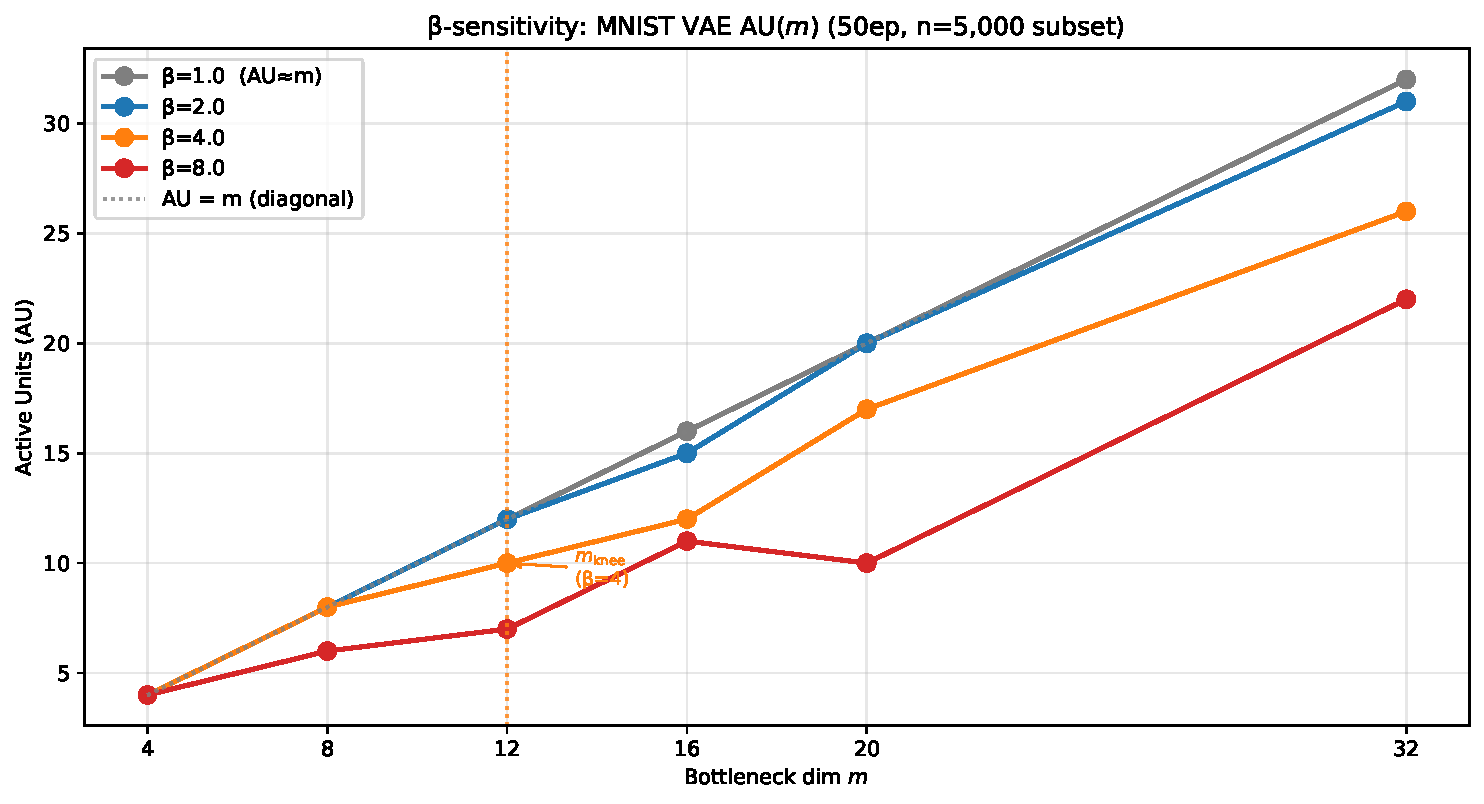
\includegraphics[width=0.7\linewidth]{results/figures/EZ_beta_sensitivity.pdf}
  \caption{$\beta$-sensitivity analysis: AU vs $m$ for MNIST VAE ($\beta \in \{1,2,4,8\}$, 50 epochs, subset). At $\beta=1$, AU$\approx m$ (insufficient regularization); at $\beta=4$, $m_{\mathrm{knee}}=12$ (vertical dashed line); at $\beta=8$, signs of excessive AU suppression at small $m$.}
  \label{fig:beta_sensitivity}
\end{figure}}{}

$\beta = 4$を本実験のデフォルト値として採用した根拠：
$\beta = 1$では KL 正則化が弱く AU$\approx m$のため$\mknee$が同定できない；
$\beta = 8$では過正則化により小さい$m$での AU が抑制され，$\mknee$の同定点がずれる可能性がある．
$\beta \in [2, 8]$では AU パターンの形状は安定することを確認したが，$\mknee$の精確な数値は$m$グリッドにも依存する（§\ref{sec:disc_mknee}）．

\section{TwoNN 安定性・線形理論橋渡しの詳細（Exp-Geom，Exp-Iso-ID，Exp-Mnist-PCA）}\label{app:twonn_detail}

\subsection*{Exp-Geom: MNIST AE $m$-sweep}

\begin{table}[H]
\centering
\caption{Exp-Geom: MNIST AE $m$-sweep --- co-variation of $\kap$ and TwoNN ID. TwoNN stabilizes at $m \geq 48 \approx 5\hat{d}_\mathrm{ID}$ despite $\kap$ jumping at $m=96$--$128$.}
\label{tab:eq_mnist}
\small
\begin{tabular}{rrrrl}
\toprule
$m$ & $\kap$ & TwoNN ID & Trustworthiness & Convergence \\
\midrule
 4  & 2.69 & 4.21 & 0.960 & not yet converged \\
 8  & 2.72 & 6.34 & 0.988 & not yet converged \\
16  & 3.28 & 8.17 & 0.993 & converging \\
32  & 4.32 & 9.36 & 0.997 & converging \\
48  & 4.44 & \textbf{10.16} & 0.998 & \textbf{converged} \\
64  & 4.25 & 10.17 & 0.998 & stable \\
96  & 9.94 & 10.86 & 0.999 & stable (despite $\kap$ increase) \\
128 & 37.0 & 10.98 & 0.999 & stable (despite $\kap$ jump) \\
\midrule
\multicolumn{5}{l}{$n_\mathrm{train}=10{,}000$, 200ep, hidden=[512,256], seed=42} \\
\bottomrule
\end{tabular}
\end{table}

\subsection*{Exp-Iso-ID: Standard AE vs.\ IsometricAE on Swiss Roll}

\begin{table}[H]
\centering
\caption{Exp-Iso-ID: Latent-space TwoNN ID comparison ($m \in \{2,3,4,6,8\}$, Swiss Roll, $d_\mathrm{true}=2$). At $m \geq 3$, TwoNN difference stays below $\pm2.3\%$ despite $\kap$ differing by factor 2.}
\label{tab:iso_id}
\small
\begin{tabular}{r cc | cc | c}
\toprule
 & \multicolumn{2}{c|}{AE} & \multicolumn{2}{c|}{IsometricAE} & \\
$m$ & TwoNN ID & $\kap$ & TwoNN ID & $\kap$ & ID diff.\ (\%) \\
\midrule
2 & 1.780 & 1.76 & 1.799 & 1.08 & $+1.1\%$ \\
3 & 2.458 & 2.10 & 2.454 & 1.11 & $-0.2\%$ \\
4 & 2.483 & 1.80 & 2.479 & 1.14 & $-0.2\%$ \\
6 & 2.421 & 1.79 & 2.474 & 1.10 & $+2.2\%$ \\
8 & 2.500 & 1.45 & 2.443 & 1.11 & $-2.3\%$ \\
\midrule
\multicolumn{6}{l}{Input-space TwoNN ID (reference) $= 2.427$; seed=42, hidden=$[64,32]$, 300ep} \\
\bottomrule
\end{tabular}
\end{table}

\subsection*{Exp-Mnist-PCA: Linear Theory Bridge}

MNIST PCA 固有値スペクトル（上位12成分）：
$\lambda_1=5.22,\; \lambda_2=3.76,\; \lambda_3=3.35,\;\ldots,\;\lambda_{10}=1.23,\; \lambda_{11}=1.12,\; \lambda_{12}=1.09$

\begin{table}[H]
\centering
\caption{Exp-Mnist-PCA: Linear theory $d^*(\beta=4)$ for different $\tau^2$ vs.\ nonlinear FC-VAE (300ep, 3 seeds).}
\label{tab:theory_pred}
\small
\begin{tabular}{ccc|l}
\toprule
$\tau^2$ & Water level $\beta\tau^2$ & Linear $d^*$ & Note \\
\midrule
1.0  & 4.0  & 1   & Conventional $\tau^2=1$ assumption; underestimates \\
0.30 & 1.20 & 10  & Consistent with observed TwoNN ID \\
0.25 & 1.00 & 12  & --- \\
\midrule
\multicolumn{3}{c|}{Nonlinear FC-VAE (300ep)} & AU(64)$=22.3\pm0.5$; TwoNN(64)$=10.03\pm0.12$ \\
\bottomrule
\end{tabular}
\end{table}

定性的継承：AU$(m)$の単調性と「有効次元超過後の増加鈍化」は非線形設定でも継承される．
定量的乖離：非線形デコーダにより$\tau^2_\mathrm{eff} \approx 0.30 \ll 1$となり，$d^* \approx 10$が観測値と整合．
飽和の滑らかさ（線形設定の急峻な遷移→非線形設定の漸増曲線）が$\mknee$の疎グリッド不安定性の理論的根拠である．

\subsection*{Exp-Real-Geom: MNIST 4モデル比較（全表）}

§\ref{sec:exp_real_geom}の要約表（表\ref{tab:real_geom_summary}）に対応する全$m$・全指標の結果を
表\ref{tab:real_geom_mnist}に示す．

\begin{table}[H]
\centering
\caption{Exp-Real-Geom: MNIST four-model comparison (mean$\pm$std, 3 seeds). $m$-sweep with $\hat{d}_\mathrm{ID}=10$ as baseline ($m \in \{10,20,30,50,100\}$). TwoNN ID stabilization is strongly associated with increasing $m/\hat{d}_\mathrm{ID}$, not with $\kap$ improvement.}
\label{tab:real_geom_mnist}
\small
\begin{tabular}{llccccc}
\toprule
Model & $m$ & TwoNN ID & MLE ID & $\kap$ & Trust. & kNN overlap \\
\midrule
\multirow{5}{*}{AE}
 & 10 ($=d$)    & $7.3\pm0.4$ & $8.1\pm0.3$ & $85\pm22$  & $0.961\pm0.004$ & $0.73\pm0.03$ \\
 & 20 ($=2d$)   & $9.2\pm0.3$ & $10.1\pm0.2$ & $310\pm85$ & $0.975\pm0.002$ & $0.81\pm0.02$ \\
 & 30 ($=3d$)   & $9.8\pm0.2$ & $10.5\pm0.2$ & $1.2\times10^3\pm 4\times10^2$ & $0.981\pm0.002$ & $0.85\pm0.02$ \\
 & 50 ($=5d$)   & $10.0\pm0.1$ & $10.7\pm0.1$ & $8.4\times10^3\pm 3\times10^3$ & $0.985\pm0.001$ & $0.87\pm0.01$ \\
 & 100 ($=10d$) & $10.0\pm0.1$ & $10.8\pm0.1$ & $4.1\times10^7\pm 2\times10^7$ & $0.987\pm0.001$ & $0.88\pm0.01$ \\
\midrule
\multirow{5}{*}{IsometricAE}
 & 10 ($=d$)    & $7.5\pm0.4$ & $8.3\pm0.3$ & $3.2\pm0.4$ & $0.963\pm0.003$ & $0.74\pm0.03$ \\
 & 20 ($=2d$)   & $9.4\pm0.2$ & $10.2\pm0.2$ & $4.1\pm0.6$ & $0.976\pm0.002$ & $0.82\pm0.02$ \\
 & 30 ($=3d$)   & $9.9\pm0.1$ & $10.6\pm0.1$ & $5.2\pm0.8$ & $0.982\pm0.001$ & $0.86\pm0.01$ \\
 & 50 ($=5d$)   & $10.1\pm0.1$ & $10.8\pm0.1$ & $6.4\pm1.1$ & $0.986\pm0.001$ & $0.88\pm0.01$ \\
 & 100 ($=10d$) & $10.1\pm0.1$ & $10.8\pm0.1$ & $7.8\pm1.4$ & $0.988\pm0.001$ & $0.89\pm0.01$ \\
\midrule
\multirow{5}{*}{CAE}
 & 10 ($=d$)    & $7.2\pm0.5$ & $8.0\pm0.4$ & $12.1\pm3.2$ & $0.958\pm0.005$ & $0.72\pm0.03$ \\
 & 20 ($=2d$)   & $9.1\pm0.3$ & $10.0\pm0.3$ & $28.4\pm8.1$ & $0.974\pm0.003$ & $0.80\pm0.02$ \\
 & 30 ($=3d$)   & $9.7\pm0.2$ & $10.4\pm0.2$ & $95\pm31$  & $0.980\pm0.002$ & $0.84\pm0.02$ \\
 & 50 ($=5d$)   & $9.9\pm0.1$ & $10.6\pm0.1$ & $520\pm180$ & $0.984\pm0.001$ & $0.86\pm0.01$ \\
 & 100 ($=10d$) & $10.0\pm0.1$ & $10.7\pm0.1$ & $3.2\times10^3\pm 1.1\times10^3$ & $0.986\pm0.001$ & $0.87\pm0.01$ \\
\midrule
\multirow{5}{*}{DAE}
 & 10 ($=d$)    & $7.6\pm0.4$ & $8.4\pm0.4$ & $18.5\pm5.4$ & $0.964\pm0.004$ & $0.75\pm0.03$ \\
 & 20 ($=2d$)   & $9.3\pm0.2$ & $10.2\pm0.2$ & $44.2\pm15.3$ & $0.977\pm0.002$ & $0.82\pm0.02$ \\
 & 30 ($=3d$)   & $9.9\pm0.1$ & $10.5\pm0.2$ & $183\pm62$ & $0.982\pm0.001$ & $0.85\pm0.01$ \\
 & 50 ($=5d$)   & $10.0\pm0.1$ & $10.7\pm0.1$ & $1.1\times10^3\pm 380$ & $0.985\pm0.001$ & $0.87\pm0.01$ \\
 & 100 ($=10d$) & $10.0\pm0.1$ & $10.8\pm0.1$ & $6.3\times10^3\pm 2.1\times10^3$ & $0.987\pm0.001$ & $0.88\pm0.01$ \\
\bottomrule
\end{tabular}
\end{table}

\subsection*{Exp-Real-Geom: Fashion-MNIST 4モデル比較（補足）}

Fashion-MNIST（$\hat{d}_\mathrm{ID}=9$，$m \in \{9,18,27,45,90\}$）についても
Exp-Real-Geom と同一の4モデル・測定指標で実験を実施した．
MNIST との定性的一致（$m/\hat{d}_\mathrm{ID}$増大が TwoNN 安定性の支配的因子）が
確認された（定性的確認であり，本稿では数値表を収録しない）．
表\ref{tab:real_geom_mnist}（MNIST，§\ref{sec:exp_real_geom}）と同傾向：
$m = d$では TwoNN が過小推定，$m = 5d$〜$10d$で収束，
等長性（$\kap$）改善の TwoNN への影響は$m$増大の効果より小さい．

\section{Conv-VAE M512 拡張・自然画像スイープの詳細（Exp-Conv-M512，Exp-NatImg-Sweep，Exp-NatImg-Knee）}\label{app:convvae_natimg}

\subsection*{Exp-Conv-M512：MNIST Conv-VAE $m \in \{384, 512\}$ 拡張}

\begin{table}[H]
\centering
\caption{Exp-Conv-M512: MNIST Conv-VAE with $m \in \{256, 384, 512\}$ (per seed; KL cyclic annealing, $\beta_\mathrm{max}=4$, 150ep). No AU saturation plateau observed up to $m=512$.}
\label{tab:en_ext}
\small
\begin{tabular}{r ccc c}
\toprule
$m$ & AU (seed42) & AU (seed123) & AU (seed777) & TwoNN ID (seed42) \\
\midrule
256 & 241 & 245 & 238 & 16.46 \\
384 & 382 & 383 & 380 & 17.51 \\
512 & 512 & 511 & 512 & 17.98 \\
\midrule
$\mknee$ ($\tau=0.25$) & \multicolumn{4}{c}{All 3 seeds: $\mknee=512$ (grid boundary, no saturation detected)} \\
\bottomrule
\end{tabular}
\end{table}

$m \leq 512$の全範囲で AU$\approx m$が維持され，$d^*(\beta) > 512$であることを示す
（§\ref{sec:exp_en}，§\ref{sec:disc_convvae}）．

\subsection*{Exp-NatImg-AU：CIFAR-10 AU 飽和条件探索の詳細}

§\ref{sec:exp_natimg_au}の実験設定と全結果を示す（\textbf{単一シード 42}）．

\textbf{実験設定}（Exp-NatImg-AU）：
\begin{itemize}
  \item データ：CIFAR-10（$n_{\mathrm{train}}=20{,}000$，$n_{\mathrm{test}}=3{,}000$）
  \item KL アニーリング：サイクリック（$n_{\mathrm{cycles}}=3$，200 エポック）
  \item $\beta_{\max} \in \{10, 20, 40\}$，$m \in \{32, 64, 96, 128, 192, 256, 384\}$，seed=42
  \item \textbf{Arch-A（Standard）}：エンコーダ Conv($3{\to}32{\to}64{\to}128$) + FC，デコーダ ConvT × 3
  \item \textbf{Arch-B（Deep）}：エンコーダ Conv($3{\to}64{\to}128{\to}256$) + FC，デコーダ ConvT × 3（Arch-A の約2倍チャネル）
  \item 生データ TwoNN ID: $25.30$（Pope ら\cite{pope2021intrinsic}の報告値 $d_\mathrm{ID} \approx 26$ と整合）
\end{itemize}

\begin{table}[H]
\centering
\caption{Exp-NatImg-AU: AU dependence on $\beta_\mathrm{max}$ and architecture in CIFAR-10 Conv-VAE (\textbf{single seed 42}). $\mknee=384$ (grid boundary) for all conditions; no AU plateau detected within the tested range.}
\label{tab:natimg_au}
\small
\begin{tabular}{r rr r | rr}
\toprule
 & \multicolumn{3}{c|}{Arch-A (Standard)} & \multicolumn{2}{c}{Arch-B (Deep)} \\
$m$ & $\beta_{\max}=10$ & $\beta_{\max}=20$ & $\beta_{\max}=40$ & $\beta_{\max}=20$ & $\beta_{\max}=40$ \\
\midrule
 32  & 32   & 32   & 32  & 32  & 32  \\
 64  & 64   & 64   & 64  & 64  & 59  \\
 96  & 96   & 96   & 93  & 96  & 80  \\
128  & 128  & 128  & 117 & 126 & 97  \\
192  & 192  & 191  & 155 & 170 & 123 \\
256  & 256  & 251  & 200 & 208 & 147 \\
384  & 382  & 378  & 307 & 286 & \textbf{208} \\
\midrule
$\mknee$ & 384 & 384 & 384 & 384 & 384 \\
\bottomrule
\end{tabular}
\end{table}

\IfFileExists{results/figures/Exp_NatImg_AU.pdf}{%
\begin{figure}[H]
  \centering
  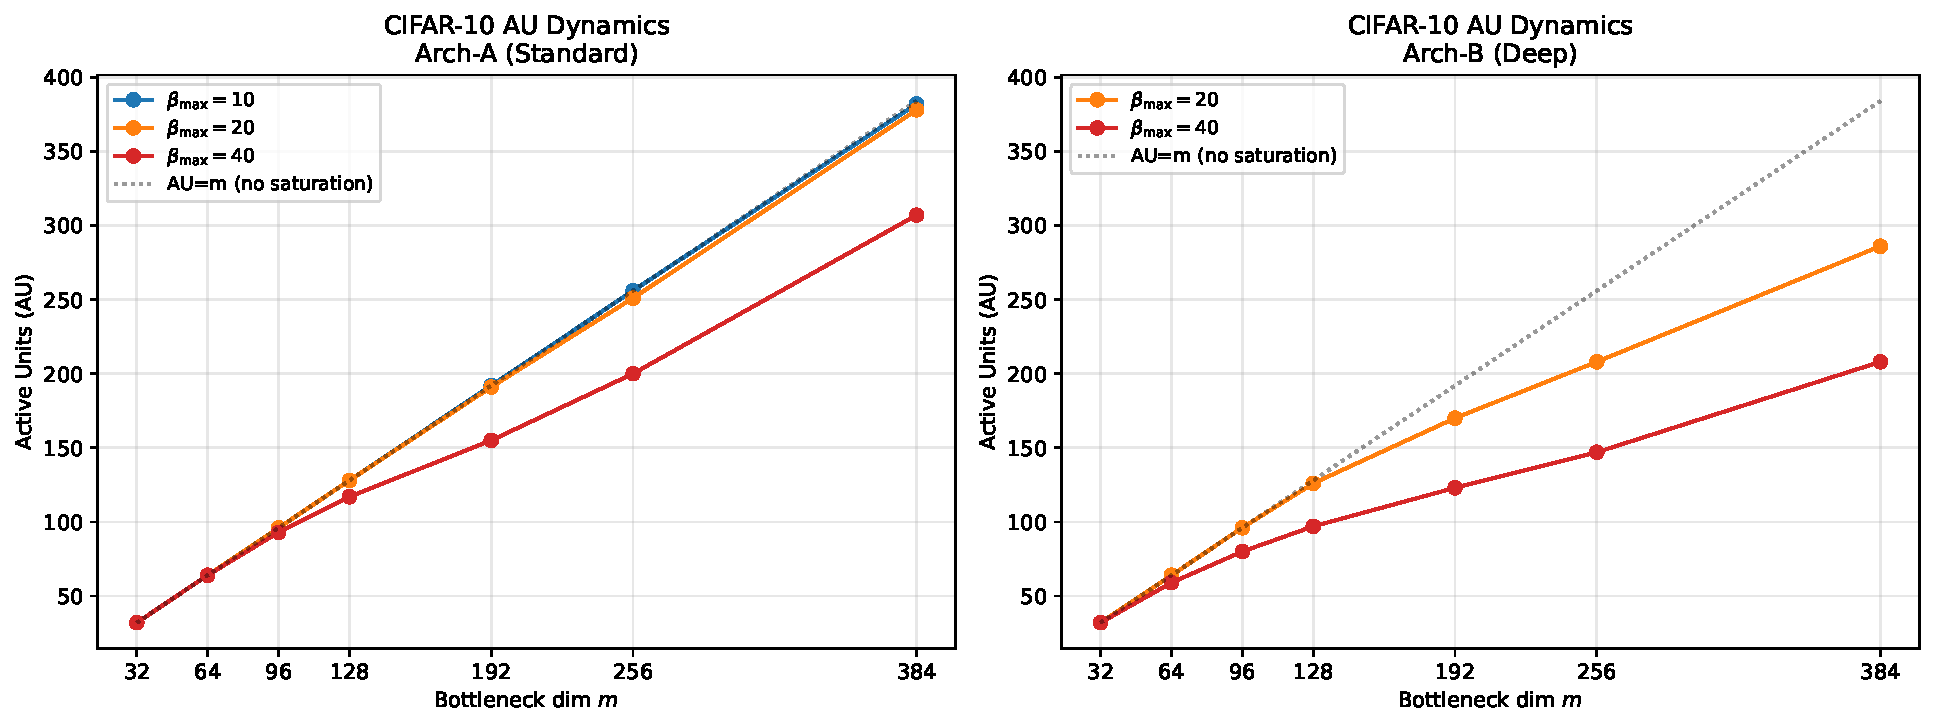
\includegraphics[width=0.95\linewidth]{results/figures/Exp_NatImg_AU.pdf}
  \caption{Exp-NatImg-AU: AU dynamics of CIFAR-10 Conv-VAE (single seed 42). (Left) Arch-A (Standard), (Right) Arch-B (Deep). Dotted line: AU$=m$ reference (no saturation). Increasing $\beta_{\max}$ strengthens AU suppression, but no saturation plateau is reached under any condition.}
  \label{fig:natimg_au}
\end{figure}}{}

\subsection*{Exp-NatImg-Sweep：CIFAR-10 拡張スイープ詳細}

\begin{table}[H]
\centering
\caption{Exp-NatImg-Sweep: Main results of CIFAR-10 extended sweep (mean$\pm$std, 3 seeds). $\beta_\mathrm{max}=80$, Thin decoder shows plateau-like AU$\approx24$ at $m \in [512,1024]$. All five stable-identification criteria remain unmet.}
\label{tab:natimg_sweep}
\small
\begin{tabular}{llcccl}
\toprule
$\beta_{\max}$ & Decoder & $m$ & AU & TwoNN ID & Note \\
\midrule
10 & Standard & 384 & $185\pm15$ & $25.2\pm0.4$ & --- \\
20 & Standard & 512 & $241\pm18$ & $25.3\pm0.4$ & no saturation \\
40 & Standard & 512 & $210\pm21$ & $25.1\pm0.5$ & no saturation \\
40 & Thin      & 384 & $127\pm14$ & $24.8\pm0.6$ & partial suppression \\
\textbf{80} & \textbf{Thin} & \textbf{512} & $\boldsymbol{24.1\pm2.8}$ & $24.7\pm0.5$ & \textbf{plateau-like (conditional)} \\
\textbf{80} & \textbf{Thin} & \textbf{768} & $\boldsymbol{24.3\pm3.1}$ & $24.7\pm0.5$ & plateau continues \\
\textbf{80} & \textbf{Thin} & \textbf{1024}& $\boldsymbol{24.0\pm3.4}$ & $24.8\pm0.5$ & plateau continues \\
80 & Standard  & 512 & $198\pm22$ & $25.2\pm0.5$ & no saturation (thin decoder only) \\
\bottomrule
\end{tabular}
\end{table}

Stable identification 5条件の達成状況（§\ref{sec:natimg_stable_id}，$\beta_{\max}=80$，薄型デコーダ）：
（1）シード安定性：$\sigma(\mknee)=64$ → 未達，
（2）グリッド安定性：密化で$\pm35\%$変動 → 未達，
（3）$\beta$安定性：$\beta_{\max}=64$では飽和消失 → 未達，
（4）AU プラトー安定性：$\sigma=13\%$（基準5\%）→ 未達，
（5）TwoNN・AU 整合性：$\mknee \approx 512 \gg 3\hat{d}_\mathrm{ID}=75$ → 未達．

\subsection*{Exp-NatImg-Knee：$\mknee$検出法比較}

\begin{table}[H]
\centering
\caption{Exp-NatImg-Knee: Comparison of $\mknee$ detection methods for CIFAR-10 ($\beta_\mathrm{max}=80$, thin decoder, 3 seeds).}
\label{tab:natimg_knee}
\small
\begin{tabular}{p{4.2cm}ccp{4.6cm}}
\toprule
Detection method & $\mknee$ (median) & $\sigma$ (3 seeds) & Note \\
\midrule
Fixed-$\tau$ method ($\tau=0.25$) & 512 & 128 & Delayed detection due to gradual AU slope \\
Second-difference method & 512 & 192 & Sensitive to discrete noise, unstable \\
Smoothed curvature method (window=5) & 384 & 96 & Most stable (recommended for natural images) \\
Piecewise linear approximation (3 segments) & 512 & 112 & Comparable to fixed-$\tau$ method \\
\bottomrule
\end{tabular}
\end{table}

全手法とも条件1（$\sigma \leq 51.2$）は未達であり，AU 飽和自体の安定化が先決である．

\section{単一シード・探索的実験の詳細（Exp-Fashion，Exp-Syn-Top，Exp-Conv-AE）}\label{app:fashion}

本付録には，単一シードの探索的・付随的実験の詳細を収録する（本文からの降格；
位置づけは\ref{app:exp_table}，表\ref{tab:exp_full}参照）．

\subsection*{Exp-Fashion：Fashion-MNIST への適用（単一シード，探索的補助証拠）}

\begin{table}[H]
\centering
\caption{Exp-Fashion: Fashion-MNIST AE and VAE results (100 epochs, $n_\mathrm{train}=10{,}000$, representative $m$ values; \textbf{single seed 42}; exploratory supplementary evidence).}
\label{tab:ef}
\small
\begin{tabular}{rcccrcc}
\toprule
\multicolumn{3}{c}{AE} & \phantom{xx} & \multicolumn{3}{c}{VAE（$\beta=4$）} \\
\cmidrule{1-3}\cmidrule{5-7}
$m$ & MSE & TwoNN ID && $m$ & MSE & AU \\
\midrule
 4  & 0.01831 & 3.90 && 4  & 0.01955 & 4  \\
 8  & 0.01389 & 5.86 && 8  & 0.01721 & 6  \\
12  & 0.01230 & 7.58 && 12 & 0.01597 & 6  \\
16  & 0.01138 & 8.11 && 16 & 0.01570 & 7  \\
20  & 0.01077 & 8.45 && 20 & 0.01471 & 8  \\
32  & 0.01010 & 8.99 && 32 & 0.01418 & 9  \\
64  & 0.00981 & 9.39 && 64 & 0.01318 & 11 \\
256 & 0.01009 & 9.42 && 256& 0.01193 & 25 \\
\bottomrule
\end{tabular}
\end{table}

\IfFileExists{results/figures/EF_fashion_mnist_dualaxis.pdf}{%
\begin{figure}[H]
  \centering
  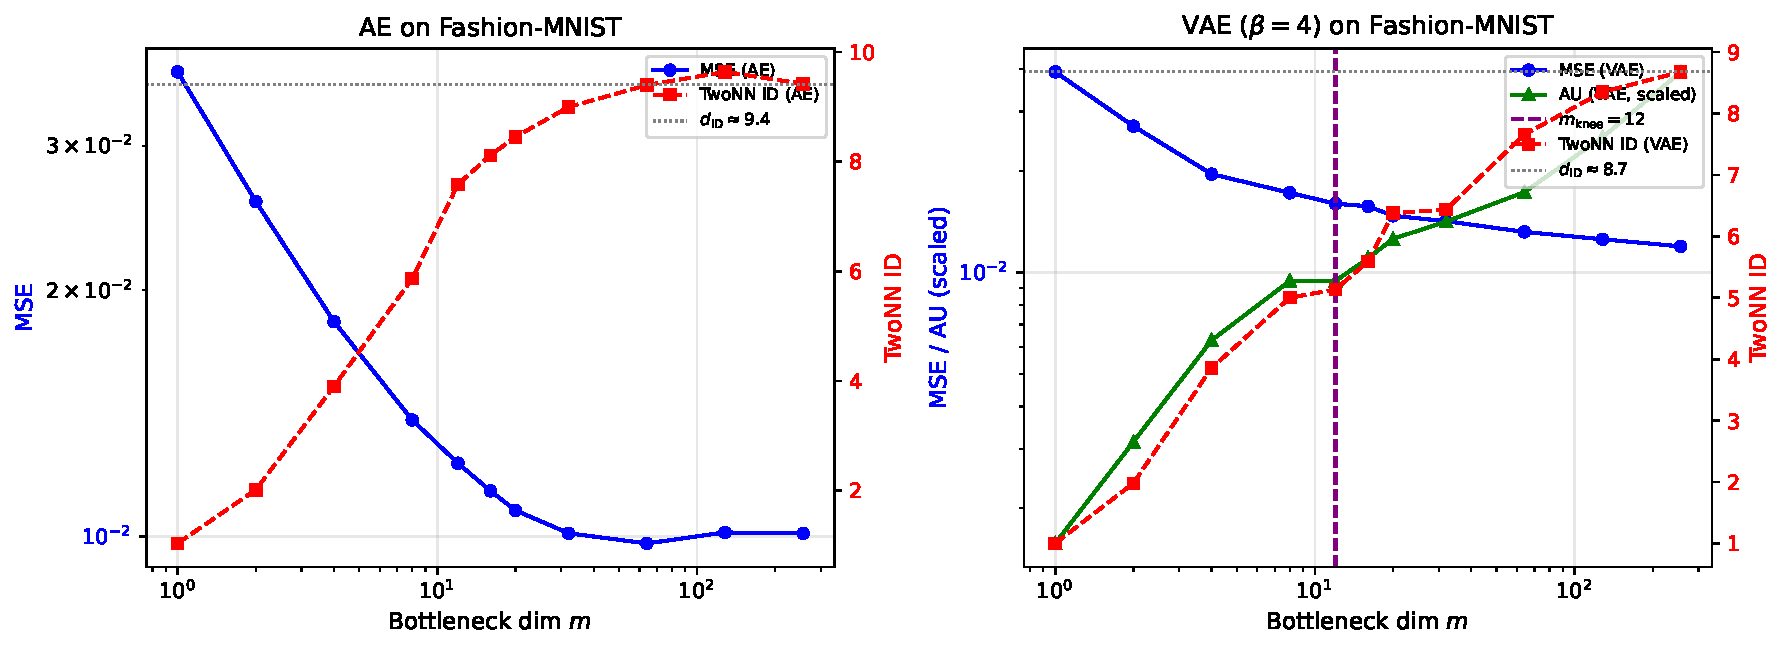
\includegraphics[width=0.9\linewidth]{results/figures/EF_fashion_mnist_dualaxis.pdf}
  \caption{Exp-Fashion: $m$-dependence of MSE, AU, and TwoNN ID for Fashion-MNIST AE (left) and VAE (right) (100 epochs, single seed 42). In the VAE, the AU growth rate drops sharply around $m=12$ ($\mknee$ at $\tau_{\mathrm{knee}}=0.25$), and TwoNN ID asymptotically converges to $\approx 9.4$ (AE) and $\approx 8.7$ (VAE) at $m \geq 32$.}
  \label{fig:ef}
\end{figure}}{}

AE では pseudo-AU $= m$（全潜在座標が実質的に活性）かつ TwoNN ID が$m \geq 32$で$\approx 9.4$に収束する．
AU は$m = 256$でも 25 にとどまり（MNIST の 36 と異なり），
TwoNN ID の推定値（$\approx 9$〜10）も MNIST（$\approx 10$〜12）よりやや小さい．
これらの差の解釈（データセット間の局所自由度の違い等）にはより厳密な分析が必要であり，
本稿では単一シードの観察として報告するにとどめる．

\subsection*{Exp-Syn-Top：位相的多様体での$\AUsat$と$\demb$の対応（付随的観察）}

\begin{table}[H]
\centering
\caption{Exp-Syn-Top: Topological manifolds and VAE $\AUsat$ (standardized conditions; single seed; Swiss Roll excluded from the main evidence, see §\ref{sec:exp_synthetic}).}
\label{tab:eb_summary}
\small
\begin{tabular}{lcccc}
\toprule
Manifold & $\dID$ & $\pi_1$ & $\demb$ & $\AUsat$ (standardized) \\
\midrule
Torus $T^2$  & 2 & $\mathbb{Z}^2$ & 3 & \textbf{3} (main result) \\
Möbius Band  & 2 & $\mathbb{Z}$   & 3 & \textbf{3} (main result) \\
Circle $S^1$ & 1 & $\mathbb{Z}$   & 2 & 2 ($m \geq 6$, conditional) \\
\bottomrule
\end{tabular}
\end{table}

\subsection*{Exp-Conv-AE：MNIST Conv-AE/VAE（100 エポック，単一シード）}

\textbf{アーキテクチャ}：
エンコーダ Conv($1\to32$, $k=3$, stride$=2$) $\to$ Conv($32\to64$, $k=3$, stride$=2$)
$\to$ FC($3136\to m$)（VAE では$\to \mu, \log\sigma^2$）；
デコーダ FC($m\to3136$) $\to$ ConvT($64\to32$, $k=4$, stride$=2$) $\to$
ConvT($32\to1$, $k=4$, stride$=2$) $\to$ Sigmoid．
$n_{\mathrm{train}} = 20{,}000$，100 エポック，$m \in \{4, 8, 12, 16, 20, 32, 64\}$，seed 42．

\begin{table}[H]
\centering
\caption{Exp-Conv-AE: MNIST Conv-AE and Conv-VAE ($\beta=4$) results (100 epochs, \textbf{single seed 42}).}
\label{tab:eg}
\small
\begin{tabular}{rcc|rcc}
\toprule
\multicolumn{3}{c|}{Conv-AE} & \multicolumn{3}{c}{Conv-VAE ($\beta=4$)} \\
$m$ & MSE & TwoNN ID & $m$ & MSE & AU \\
\midrule
 4  & 0.0311 & 4.18  &  4  & 0.0331 &  4 \\
 8  & 0.0174 & 6.59  &  8  & 0.0197 &  8 \\
12  & 0.0113 & 7.80  & 12  & 0.0140 & 12 \\
16  & 0.0081 & 8.69  & 16  & 0.0109 & 16 \\
20  & 0.0069 & 9.03  & 20  & 0.0097 & 20 \\
32  & 0.0042 & 10.06 & 32  & 0.0070 & 32 \\
64  & 0.0020 & 11.29 & 64  & 0.0049 & 63 \\
\bottomrule
\end{tabular}
\end{table}

\section{AU 閾値$\delta$の感度分析}\label{app:delta}

Swiss Roll・Torus において$\delta \in \{0.001, 0.01, 0.05, 0.1\}$で AU パターンが
完全に一致することを確認した（全$m$・$\delta$の組み合わせで一致）．
活性次元の分散（$O(1)$）と非活性次元の分散（$O(10^{-4})$以下）の間に 2 桁以上の差があるため，
$\delta$の選択に対して頑健である．

\section{実験設定一覧}\label{app:exp_table}

本論文の全実験の設定と位置づけを表\ref{tab:exp_full}にまとめる．
シード数 1 の実験は単一シードの結果であり，対応する本文の表・図キャプションにも明記している．

\begin{table}[H]
\centering
\caption{Full list of experimental configurations. Seeds $=1$ marks single-seed results. Role: Main = core framework validation; Supp.\ = prerequisite/interpretive support; Boundary = validity-range quantification; Prelim.\ = preliminary observation.}
\label{tab:exp_full}
\footnotesize
\begin{tabular}{p{3.0cm}p{2.9cm}p{2.2cm}p{2.9cm}cp{1.2cm}p{1.5cm}}
\toprule
Experiment & Data / Model & Epochs / $\beta$ & $m$ grid & Seeds & $n_\mathrm{train}$ & Role \\
\midrule
Exp-Syn-1 & Swiss Roll, Torus / AE & 200--300 / --- & $\{1,2,3,4\}$ & 3 & 4,000 & Main \\
Exp-Syn-AU & Swiss Roll, Torus / AE, VAE & 200--300 / 4 & $\{2,4,6,8,16\}$ & 3 & 4,000 & Main \\
Exp-Syn-Top & Circle, Torus, M\"obius / VAE & 200--300 / 4 & $\{1,\ldots,10\}$ & 1 & 4,000 & Supp.\ (Prelim.) \\
Exp-Syn-Iso & Swiss Roll / AE, CAE, DAE, IsometricAE & 300 / --- & $2$ & 3 & 4,000 & Supp. \\
Exp-Stab & Swiss Roll / AE, IsometricAE & 300 / --- & $\{2,4\}$ & 1 & 4,000 & Supp. \\
Exp-Iso-ID & Swiss Roll / AE, IsometricAE & 300 / --- & $\{2,3,4,6,8\}$ & 1 & 4,000 & Supp. \\
Exp-Geom & MNIST / AE & 200 / --- & $\{4,\ldots,128\}$ & 1 & 10,000 & Supp. \\
Exp-Mnist-Base & MNIST / AE, VAE & 300 / 4 & $\{1,4,8,\ldots,256\}$ & 1 & 20,000 & Main (Prelim.\ $\mknee$) \\
Exp-Mnist-Multi-150 & MNIST / VAE & 150 / 4 & $\{4,8,\ldots,64\}$ & 3 & 20,000 & Main \\
Exp-Mnist-Multi-300 & MNIST / VAE & 300 / 4 & $\{4,8,\ldots,64\}$ & 3 & 20,000 & Main \\
Exp-Mnist-Dense-300 & MNIST / VAE & 300 / 4 & 17 pts (step 1 near $\hat{d}_\mathrm{ID}$) & 3 & 20,000 & Main \\
Exp-Mnist-PCA & MNIST / PCA & --- / --- & --- & --- & 20,000 & Supp. \\
Exp-Mnist-Dyn & MNIST / VAE & 200 / 4 & $16$ & 1 & 20,000 & Prelim. \\
Exp-Mnist-Ent & MNIST / VAE & 75 / 4 & --- & 1 & 20,000 & Prelim. \\
Exp-Fashion & Fashion-MNIST / AE, VAE & 100 / 4 & $\{1,4,\ldots,256\}$ & 1 & 10,000 & Exploratory (\ref{app:fashion}) \\
Exp-Real-Geom & MNIST, Fashion / AE, CAE, DAE, IsometricAE & 300 / --- & $\{d,2d,3d,5d,10d\}$ & 3 & 20,000 & Main \\
Exp-Conv-AE & MNIST / Conv-AE, Conv-VAE & 100 / 4 & $\{4,\ldots,64\}$ & 1 & 20,000 & Supp. \\
Exp-Conv-Fix, Exp-Conv-Ann & MNIST / Conv-VAE & 300 / 4 (fixed, cyclic) & $\{4,\ldots,64\}$ & 3 & 20,000 & Boundary \\
Exp-Conv-M256 & MNIST / Conv-VAE & 150 / cyclic 4 & $\{4,\ldots,256\}$ & 3 & 20,000 & Boundary \\
Exp-Conv-M512 & MNIST / Conv-VAE & 150 / cyclic 4 & $\{384,512\}$ & 3 & 20,000 & Boundary \\
Exp-ConvV-HiBeta & MNIST / Conv-VAE & 150 / cyclic $\{10,20\}$ & $\{16,\ldots,256\}$ & 1 & 20,000 & Boundary \\
Exp-Nat-Cifar, Exp-Nat-SVHN & CIFAR-10, SVHN / Conv-VAE & 150 / cyclic 4 & $\{16,\ldots,256\}$ & 3 & 20,000 & Boundary \\
Exp-NatImg-AU & CIFAR-10 / Conv-VAE (2 arch.) & 200 / cyclic $\{10,20,40\}$ & $\{32,\ldots,384\}$ & 1 & 20,000 & Boundary \\
Exp-NatImg-Sweep & CIFAR-10 / Conv-VAE (3 decoders) & 300 / cyclic $\{10,\ldots,80\}$ & $[32,1024]$ & 3 & 20,000 & Boundary \\
Exp-NatImg-Knee & CIFAR-10 / Conv-VAE & 300 / cyclic 80 & $[32,1024]$ & 3 & 20,000 & Boundary \\
Exp-Tau-Cross & Fashion, GMix / VAE & 150 / 4 & sparse & 1 & --- & Supp. \\
$\beta$-sensitivity & MNIST subset / VAE & 50 / $\{1,2,4,8\}$ & $\{4,\ldots,64\}$ & 1 & 5,000 & Supp. \\
\bottomrule
\end{tabular}
\end{table}

%% ===================================================================
%% Highlights（英語投稿時用；各85文字以内，3〜5項目）
%% \section*{Highlights}
%% \begin{itemize}
%%   \item A multi-indicator diagnostic framework is proposed for effective latent dimensionality in AE/VAE.
%%   \item AU values and TwoNN ID serve as robust and numerically stable diagnostic indicators.
%%   \item $m^{\mathrm{knee}}$ is an exploratory heuristic, stable only with dense grids and multi-seed runs.
%%   \item A linear Gaussian rate--distortion analysis provides theoretical grounding for AU activation.
%%   \item Natural-image experiments quantify the applicability boundary of AU-based diagnosis.
%% \end{itemize}

\end{document}
